\documentclass[12pt,fleqn]{book} % Default font size and left-justified equations

%----------------------------------------------------------------------------------------
%	VARIOUS REQUIRED PACKAGES AND CONFIGURATIONS
%----------------------------------------------------------------------------------------

\usepackage[top=3cm,bottom=3cm,left=3cm,right=3cm,headsep=10pt,a4paper]{geometry} % Page margins

\usepackage{subcaption}
\usepackage{graphicx} % Required for including pictures
\graphicspath{{includes/pictures/}} % Specifies the directory where pictures are stored

\usepackage[american]{circuitikz} %Allow to draw circuit elements.

\usepackage{multicol}
\usepackage{python}
\usepackage{setspace}
\usepackage{newfloat}
\usepackage{mathrsfs}
\usepackage{lipsum} % Inserts dummy text

\usepackage[final]{pdfpages} % Allow insert PDF documents in the pages.

\usepackage{indentfirst} % Inserts a blank space in the begining of each paragraph

\usepackage{tikz} % Required for drawing custom shapes

\usepackage[brazilian]{babel} % Portuguese language/hyphenation

\usepackage[utf8]{inputenc}
\usepackage[T1]{fontenc}

\usepackage{sectsty}

\usepackage{enumitem} % Customize lists
\setlist{nolistsep} % Reduce spacing between bullet points and numbered lists

\usepackage{booktabs} % Required for nicer horizontal rules in tables

\usepackage{xcolor} % Required for specifying colors by name
\definecolor{ocre}{RGB}{119,136,153} % Define the orange color used for highlighting throughout the book

%----------------------------------------------------------------------------------------
%	FONTS
%----------------------------------------------------------------------------------------

\usepackage{avant} % Use the Avantgarde font for headings
%\usepackage{times} % Use the Times font for headings
\usepackage{mathptmx} % Use the Adobe Times Roman as the default text font together with math symbols from the Sym­bol, Chancery and Com­puter Modern fonts

\usepackage{microtype} % Slightly tweak font spacing for aesthetics
\usepackage[utf8]{inputenc} % Required for including letters with accents
\usepackage[T1]{fontenc} % Use 8-bit encoding that has 256 glyphs

%----------------------------------------------------------------------------------------
%	BIBLIOGRAPHY AND INDEX
%----------------------------------------------------------------------------------------

\usepackage[style=alphabetic,citestyle=numeric,sorting=nyt,sortcites=true,autopunct=true,babel=hyphen,hyperref=true,abbreviate=false,backref=true,backend=biber]{biblatex}
\addbibresource{bibliography.bib} % BibTeX bibliography file
\defbibheading{bibempty}{}

\usepackage{calc} % For simpler calculation - used for spacing the index letter headings correctly
\usepackage{makeidx} % Required to make an index
\makeindex % Tells LaTeX to create the files required for indexing

%----------------------------------------------------------------------------------------
%	MAIN TABLE OF CONTENTS
%----------------------------------------------------------------------------------------

\usepackage{titletoc} % Required for manipulating the table of contents

\contentsmargin{0cm} % Removes the default margin

% Part text styling
\titlecontents{part}[0cm]
{\addvspace{20pt}\centering\large\bfseries}
{}
{}
{}

% Chapter text styling
\titlecontents{chapter}[1.25cm] % Indentation
{\addvspace{12pt}\large\sffamily\bfseries} % Spacing and font options for chapters
{\color{ocre!60}\contentslabel[\Large\thecontentslabel]{1.25cm}\color{ocre}} % Chapter number
{\color{ocre}}  
{\color{ocre}\normalsize\;\titlerule*[.5pc]{.}\;\thecontentspage} % Page number


% Section text styling
\titlecontents{section}[1.25cm] % Indentation
{\addvspace{3pt}\sffamily\bfseries} % Spacing and font options for sections
{\contentslabel[\thecontentslabel]{1.25cm}} % Section number
{}
{\hfill\color{black}\thecontentspage} % Page number
[]

% Subsection text styling
\titlecontents{subsection}[1.25cm] % Indentation
{\addvspace{1pt}\sffamily\small} % Spacing and font options for subsections
{\contentslabel[\thecontentslabel]{1.25cm}} % Subsection number
{}
{\ \titlerule*[.5pc]{.}\;\thecontentspage} % Page number
[]
% List of figures
\titlecontents{figure}[0em]
{\addvspace{-5pt}\sffamily}
{\thecontentslabel\hspace*{1em}}
{}
{\ \titlerule*[.5pc]{.}\;\thecontentspage}
[]

% List of tables
\titlecontents{table}[0em]
{\addvspace{-5pt}\sffamily}
{\thecontentslabel\hspace*{1em}}
{}
{\ \titlerule*[.5pc]{.}\;\thecontentspage}
[]

%----------------------------------------------------------------------------------------
%	MINI TABLE OF CONTENTS IN PART HEADS
%----------------------------------------------------------------------------------------

% Chapter text styling
\titlecontents{lchapter}[0em] % Indenting
{\addvspace{15pt}\large\sffamily\bfseries} % Spacing and font options for chapters
{\color{ocre}\contentslabel[\Large\thecontentslabel]{1.25cm}\color{ocre}} % Chapter number
{}  
{\color{ocre}\normalsize\sffamily\bfseries\;\titlerule*[.5pc]{.}\;\thecontentspage} % Page number

% Section text styling
\titlecontents{lsection}[0em] % Indenting
{\sffamily\small} % Spacing and font options for sections
{\contentslabel[\thecontentslabel]{1.25cm}} % Section number
{}
{}

% Subsection text styling
\titlecontents{lsubsection}[.5em] % Indentation
{\normalfont\footnotesize\sffamily} % Font settings
{}
{}
{}

%----------------------------------------------------------------------------------------
%	PAGE HEADERS
%----------------------------------------------------------------------------------------

\usepackage{fancyhdr} % Required for header and footer configuration

\pagestyle{fancy}
\renewcommand{\chaptermark}[1]{\markboth{\sffamily\normalsize\bfseries\chaptername\ \thechapter.\ #1}{}} % Chapter text font settings
\renewcommand{\sectionmark}[1]{\markright{\sffamily\normalsize\thesection\hspace{5pt}#1}{}} % Section text font settings
\fancyhf{} \fancyhead[LE,RO]{\sffamily\normalsize\thepage} % Font setting for the page number in the header
\fancyhead[LO]{\rightmark} % Print the nearest section name on the left side of odd pages
\fancyhead[RE]{\leftmark} % Print the current chapter name on the right side of even pages
\renewcommand{\headrulewidth}{0.5pt} % Width of the rule under the header
\addtolength{\headheight}{2.5pt} % Increase the spacing around the header slightly
\renewcommand{\footrulewidth}{0pt} % Removes the rule in the footer
\fancypagestyle{plain}{\fancyhead{}\renewcommand{\headrulewidth}{0pt}} % Style for when a plain pagestyle is specified

% Removes the header from odd empty pages at the end of chapters
\makeatletter
\renewcommand{\cleardoublepage}{
\clearpage\ifodd\c@page\else
\hbox{}
\vspace*{\fill}
\thispagestyle{empty}
\newpage
\fi}

%----------------------------------------------------------------------------------------
%	THEOREM STYLES
%----------------------------------------------------------------------------------------

\usepackage{amsmath,amsfonts,amssymb,amsthm} % For math equations, theorems, symbols, etc

\newcommand{\intoo}[2]{\mathopen{]}#1\,;#2\mathclose{[}}
\newcommand{\ud}{\mathop{\mathrm{{}d}}\mathopen{}}
\newcommand{\intff}[2]{\mathopen{[}#1\,;#2\mathclose{]}}
\newtheorem{notation}{Notation}[chapter]

% Boxed/framed environments
\newtheoremstyle{ocrenumbox}% % Theorem style name
{0pt}% Space above
{0pt}% Space below
{\normalfont}% % Body font
{}% Indent amount
{\small\bf\sffamily\color{ocre}}% % Theorem head font
{\;}% Punctuation after theorem head
{0.25em}% Space after theorem head
{\small\sffamily\color{ocre}\thmname{#1}\nobreakspace\thmnumber{\@ifnotempty{#1}{}\@upn{#2}}% Theorem text (e.g. Theorem 2.1)
\thmnote{\nobreakspace\the\thm@notefont\sffamily\bfseries\color{black}---\nobreakspace#3.}} % Optional theorem note
\renewcommand{\qedsymbol}{$\blacksquare$}% Optional qed square

\newtheoremstyle{blacknumex}% Theorem style name
{5pt}% Space above
{5pt}% Space below
{\normalfont}% Body font
{} % Indent amount
{\small\bf\sffamily}% Theorem head font
{\;}% Punctuation after theorem head
{0.25em}% Space after theorem head
{\small\sffamily{\tiny\ensuremath{\blacksquare}}\nobreakspace\thmname{#1}\nobreakspace\thmnumber{\@ifnotempty{#1}{}\@upn{#2}}% Theorem text (e.g. Theorem 2.1)
\thmnote{\nobreakspace\the\thm@notefont\sffamily\bfseries---\nobreakspace#3.}}% Optional theorem note

\newtheoremstyle{blacknumbox} % Theorem style name
{0pt}% Space above
{0pt}% Space below
{\normalfont}% Body font
{}% Indent amount
{\small\bf\sffamily}% Theorem head font
{\;}% Punctuation after theorem head
{0.25em}% Space after theorem head
{\small\sffamily\thmname{#1}\nobreakspace\thmnumber{\@ifnotempty{#1}{}\@upn{#2}}% Theorem text (e.g. Theorem 2.1)
\thmnote{\nobreakspace\the\thm@notefont\sffamily\bfseries---\nobreakspace#3.}}% Optional theorem note

% Non-boxed/non-framed environments
\newtheoremstyle{ocrenum}% % Theorem style name
{5pt}% Space above
{5pt}% Space below
{\normalfont}% % Body font
{}% Indent amount
{\small\bf\sffamily\color{ocre}}% % Theorem head font
{\;}% Punctuation after theorem head
{0.25em}% Space after theorem head
{\small\sffamily\color{ocre}\thmname{#1}\nobreakspace\thmnumber{\@ifnotempty{#1}{}\@upn{#2}}% Theorem text (e.g. Theorem 2.1)
\thmnote{\nobreakspace\the\thm@notefont\sffamily\bfseries\color{black}---\nobreakspace#3.}} % Optional theorem note
\renewcommand{\qedsymbol}{$\blacksquare$}% Optional qed square
\makeatother

% Defines the theorem text style for each type of theorem to one of the three styles above
\newcounter{dummy} 
\numberwithin{dummy}{section}
\theoremstyle{ocrenumbox}
\newtheorem{theoremeT}[dummy]{Teorema}
\newtheorem{problem}{Problem}[chapter]
\newtheorem{exerciseT}{Exercise}[chapter]
\theoremstyle{blacknumex}
\newtheorem{exampleT}{Exemplo}[chapter]
\theoremstyle{blacknumbox}
\newtheorem{vocabulary}{Vocabulary}[chapter]
\newtheorem{definitionT}{Definição}[section]
\newtheorem{corollaryT}[dummy]{Corollary}
\theoremstyle{ocrenum}
\newtheorem{proposition}[dummy]{Proposition}

%----------------------------------------------------------------------------------------
%	DEFINITION OF COLORED BOXES
%----------------------------------------------------------------------------------------

\RequirePackage[framemethod=default]{mdframed} % Required for creating the theorem, definition, exercise and corollary boxes

% Theorem box
\newmdenv[skipabove=7pt,
skipbelow=7pt,
backgroundcolor=black!5,
linecolor=ocre,
innerleftmargin=5pt,
innerrightmargin=5pt,
innertopmargin=5pt,
leftmargin=0cm,
rightmargin=0cm,
innerbottommargin=5pt]{tBox}

% Exercise box	  
\newmdenv[skipabove=7pt,
skipbelow=7pt,
rightline=false,
leftline=true,
topline=false,
bottomline=false,
backgroundcolor=ocre!10,
linecolor=ocre,
innerleftmargin=5pt,
innerrightmargin=5pt,
innertopmargin=5pt,
innerbottommargin=5pt,
leftmargin=0cm,
rightmargin=0cm,
linewidth=4pt]{eBox}	

% Definition box
\newmdenv[skipabove=7pt,
skipbelow=7pt,
rightline=false,
leftline=true,
topline=false,
bottomline=false,
linecolor=ocre,
innerleftmargin=5pt,
innerrightmargin=5pt,
innertopmargin=0pt,
leftmargin=0cm,
rightmargin=0cm,
linewidth=4pt,
innerbottommargin=0pt]{dBox}	

% Corollary box
\newmdenv[skipabove=7pt,
skipbelow=7pt,
rightline=false,
leftline=true,
topline=false,
bottomline=false,
linecolor=gray,
backgroundcolor=black!5,
innerleftmargin=5pt,
innerrightmargin=5pt,
innertopmargin=5pt,
leftmargin=0cm,
rightmargin=0cm,
linewidth=4pt,
innerbottommargin=5pt]{cBox}

% Creates an environment for each type of theorem and assigns it a theorem text style from the "Theorem Styles" section above and a colored box from above
\newenvironment{theorem}{\begin{tBox}\begin{theoremeT}}{\end{theoremeT}\end{tBox}}
\newenvironment{exercise}{\begin{eBox}\begin{exerciseT}}{\hfill{\color{ocre}\tiny\ensuremath{\blacksquare}}\end{exerciseT}\end{eBox}}				  
\newenvironment{definition}{\begin{dBox}\begin{definitionT}}{\end{definitionT}\end{dBox}}	
\newenvironment{example}{\begin{exampleT}}{\hfill{\tiny\ensuremath{\blacksquare}}\end{exampleT}}		
\newenvironment{corollary}{\begin{cBox}\begin{corollaryT}}{\end{corollaryT}\end{cBox}}	

%----------------------------------------------------------------------------------------
%	REMARK ENVIRONMENT
%----------------------------------------------------------------------------------------

\newenvironment{remark}{\par\vspace{10pt}\small % Vertical white space above the remark and smaller font size
\begin{list}{}{
\leftmargin=35pt % Indentation on the left
\rightmargin=25pt}\item\ignorespaces % Indentation on the right
\makebox[-2.5pt]{\begin{tikzpicture}[overlay]
\node[draw=ocre!60,line width=1pt,circle,fill=ocre!25,font=\sffamily\bfseries,inner sep=2pt,outer sep=0pt] at (-15pt,0pt){\textcolor{ocre}{R}};\end{tikzpicture}} % Orange R in a circle
\advance\baselineskip -1pt}{\end{list}\vskip5pt} % Tighter line spacing and white space after remark

%----------------------------------------------------------------------------------------
%	SECTION NUMBERING IN THE MARGIN
%----------------------------------------------------------------------------------------

\makeatletter
\renewcommand{\@seccntformat}[1]{\llap{\textcolor{ocre}{\csname the#1\endcsname}\hspace{1em}}}                    
\renewcommand{\section}{\@startsection{section}{1}{\z@}
{-4ex \@plus -1ex \@minus -.4ex}
{1ex \@plus.2ex }
{\normalfont\large\sffamily\bfseries}}
\renewcommand{\subsection}{\@startsection {subsection}{2}{\z@}
{-3ex \@plus -0.1ex \@minus -.4ex}
{0.5ex \@plus.2ex }
{\normalfont\sffamily\bfseries}}
\renewcommand{\subsubsection}{\@startsection {subsubsection}{3}{\z@}
{-2ex \@plus -0.1ex \@minus -.2ex}
{.2ex \@plus.2ex }
{\normalfont\small\sffamily\bfseries}}                        
\renewcommand\paragraph{\@startsection{paragraph}{4}{\z@}
{-2ex \@plus-.2ex \@minus .2ex}
{.1ex}
{\normalfont\small\sffamily\bfseries}}

%----------------------------------------------------------------------------------------
%	PART HEADINGS
%----------------------------------------------------------------------------------------

% numbered part in the table of contents
\newcommand{\@mypartnumtocformat}[2]{%
\setlength\fboxsep{0pt}%
\noindent\colorbox{ocre!20}{\strut\parbox[c][.7cm]{\ecart}{\color{ocre!70}\Large\sffamily\bfseries\centering#1}}\hskip\esp\colorbox{ocre!40}{\strut\parbox[c][.7cm]{\linewidth-\ecart-\esp}{\Large\sffamily\centering#2}}}%
%%%%%%%%%%%%%%%%%%%%%%%%%%%%%%%%%%
% unnumbered part in the table of contents
\newcommand{\@myparttocformat}[1]{%
\setlength\fboxsep{0pt}%
\noindent\colorbox{ocre!40}{\strut\parbox[c][.7cm]{\linewidth}{\Large\sffamily\centering#1}}}%
%%%%%%%%%%%%%%%%%%%%%%%%%%%%%%%%%%
\newlength\esp
\setlength\esp{4pt}
\newlength\ecart
\setlength\ecart{1.2cm-\esp}
\newcommand{\thepartimage}{}%
\newcommand{\partimage}[1]{\renewcommand{\thepartimage}{#1}}%
\def\@part[#1]#2{%
\ifnum \c@secnumdepth >-2\relax%
\refstepcounter{part}%
\addcontentsline{toc}{part}{\texorpdfstring{\protect\@mypartnumtocformat{\thepart}{#1}}{\partname~\thepart\ ---\ #1}}
\else%
\addcontentsline{toc}{part}{\texorpdfstring{\protect\@myparttocformat{#1}}{#1}}%
\fi%
\startcontents%
\markboth{}{}%
{\thispagestyle{empty}%
\begin{tikzpicture}[remember picture,overlay]%
\node at (current page.north west){\begin{tikzpicture}[remember picture,overlay]%	
\fill[ocre!20](0cm,0cm) rectangle (\paperwidth,-\paperheight);
\node[anchor=north] at (4cm,-3.25cm){\color{ocre!40}\fontsize{220}{100}\sffamily\bfseries\@Roman\c@part}; 
\node[anchor=south east] at (\paperwidth-1cm,-\paperheight+1cm){\parbox[t][][t]{8.5cm}{
\printcontents{l}{0}{\setcounter{tocdepth}{1}}%
}};
\node[anchor=north east] at (\paperwidth-1.5cm,-3.25cm){\parbox[t][][t]{15cm}{\strut\raggedleft\color{white}\fontsize{30}{30}\sffamily\bfseries#2}};
\end{tikzpicture}};
\end{tikzpicture}}%
\@endpart}
\def\@spart#1{%
\startcontents%
\phantomsection
{\thispagestyle{empty}%
\begin{tikzpicture}[remember picture,overlay]%
\node at (current page.north west){\begin{tikzpicture}[remember picture,overlay]%	
\fill[ocre!20](0cm,0cm) rectangle (\paperwidth,-\paperheight);
\node[anchor=north east] at (\paperwidth-1.5cm,-3.25cm){\parbox[t][][t]{15cm}{\strut\raggedleft\color{white}\fontsize{30}{30}\sffamily\bfseries#1}};
\end{tikzpicture}};
\end{tikzpicture}}
\addcontentsline{toc}{part}{\texorpdfstring{%
\setlength\fboxsep{0pt}%
\noindent\protect\colorbox{ocre!40}{\strut\protect\parbox[c][.7cm]{\linewidth}{\Large\sffamily\protect\centering #1\quad\mbox{}}}}{#1}}%
\@endpart}
\def\@endpart{\vfil\newpage
\if@twoside
\if@openright
\null
\thispagestyle{empty}%
\newpage
\fi
\fi
\if@tempswa
\twocolumn
\fi}

%----------------------------------------------------------------------------------------
%	CHAPTER HEADINGS
%----------------------------------------------------------------------------------------

\newcommand{\thechapterimage}{}%
\newcommand{\chapterimage}[1]{\renewcommand{\thechapterimage}{#1}}%
\def\@makechapterhead#1{%
{\parindent \z@ \raggedright \normalfont
\ifnum \c@secnumdepth >\m@ne
\if@mainmatter
\begin{tikzpicture}[remember picture,overlay]
\node at (current page.north west)
{\begin{tikzpicture}[remember picture,overlay]
\node[anchor=north west,inner sep=0pt] at (0,0) {\includegraphics[width=\paperwidth]{\thechapterimage}};
\draw[anchor=west] (\Gm@lmargin,-9cm) node [line width=2pt,rounded corners=15pt,draw=ocre,fill=ocre,fill opacity=0.9,inner sep=15pt]{\strut\makebox[22cm]{}};
\draw[anchor=west] (\Gm@lmargin+.3cm,-9cm) node {\huge\sffamily\bfseries\color{white}\thechapter. #1\strut};
\end{tikzpicture}};
\end{tikzpicture}
\else
\begin{tikzpicture}[remember picture,overlay]
\node at (current page.north west)
{\begin{tikzpicture}[remember picture,overlay]
\node[anchor=north west,inner sep=0pt] at (0,0) {\includegraphics[width=\paperwidth]{\thechapterimage}};
\draw[anchor=west] (\Gm@lmargin,-9cm) node [line width=2pt,rounded corners=15pt,draw=ocre,fill=white,fill opacity=0.9,inner sep=15pt]{\strut\makebox[22cm]{}};
\draw[anchor=west] (\Gm@lmargin+.3cm,-9cm) node {\huge\sffamily\bfseries\color{black}#1\strut};
\end{tikzpicture}};
\end{tikzpicture}
\fi\fi\par\vspace*{270\p@}}}

\DeclareFloatingEnvironment[fileext=frm,placement={b!},chapterlistsgaps=off,within=none,name=PROVA]{test}
\captionsetup[test]{labelfont=bf}

\newcommand{\addPastTest}[3]{\IfFileExists{./inclues/documents/#1/#2_#3.pdf}{\includepdf[pages=-,pagecommand={\thispagestyle{empty}\null\vspace{22.06cm}\captionof*{test}{PROVA #2.#3}}]{./includes/documents/#1/#2_#3.pdf}}{}}

%-------------------------------------------

\def\@makeschapterhead#1{%
\begin{tikzpicture}[remember picture,overlay]
\node at (current page.north west)
{\begin{tikzpicture}[remember picture,overlay]
\node[anchor=north west,inner sep=0pt] at (0,0) {\includegraphics[width=\paperwidth]{\thechapterimage}};
\draw[anchor=west] (\Gm@lmargin,-9cm) node [line width=2pt,rounded corners=15pt,draw=ocre,fill=ocre,fill opacity=0.9,inner sep=15pt]{\strut\makebox[22cm]{}};
\draw[anchor=west] (\Gm@lmargin+.3cm,-9cm) node {\huge\sffamily\bfseries\color{white}#1\strut};
\end{tikzpicture}};
\end{tikzpicture}
\par\vspace*{270\p@}}
\makeatother

%----------------------------------------------------------------------------------------
%	HYPERLINKS IN THE DOCUMENTS
%----------------------------------------------------------------------------------------

\usepackage{hyperref}
\hypersetup{hidelinks,backref=true,pagebackref=true,hyperindex=true,colorlinks=false,breaklinks=true,urlcolor= ocre,bookmarks=true,bookmarksopen=false,pdftitle={Title},pdfauthor={Author}}
\usepackage{bookmark}
\bookmarksetup{
open,
numbered,
addtohook={%
\ifnum\bookmarkget{level}=0 % chapter
\bookmarksetup{bold}%
\fi
\ifnum\bookmarkget{level}=-1 % part
\bookmarksetup{color=ocre,bold}%
\fi
}
}
%----------------------------------------------------------------------------------------
%	LAPLACE TABLE
%----------------------------------------------------------------------------------------
\newcounter{NumberInTable}
\newcommand{\LTNUM}{\stepcounter{NumberInTable}{(\theNumberInTable)}}

\newcommand{\Laplace}[1]{\ensuremath{\mathcal{L}{\left[#1\right]}}}
\newcommand{\InvLap}[1]{\ensuremath{\mathcal{L}^{-1}{\left[#1\right]}}} % Insert the commands.tex file which contains the majority of the structure behind the template

\begin{document}

%----------------------------------------------------------------------------------------
%	TITLE PAGE
%----------------------------------------------------------------------------------------

\begingroup
\thispagestyle{empty}
\begin{tikzpicture}[remember picture,overlay]
\coordinate [below=12cm] (midpoint) at (current page.north);
\node at (current page.north west)
{\begin{tikzpicture}[remember picture,overlay]
\node[anchor=north west,inner sep=0pt] at (0,0) {\includegraphics[width=\paperwidth]{includes/documents/background.pdf}}; % Background image
\draw[anchor=north] (midpoint) node [fill=ocre!30!white,fill opacity=0.0,text opacity=1,inner sep=1cm]{\Huge\centering\bfseries\sffamily\parbox[c][][t]{\paperwidth}{\centering Análise de Circuitos Elétricos\\[15pt] % Book title
{\Large{ Regime transitório}}\\[20pt] % Subtitle
{ Sydeney Araujo}}}; % Author name
\end{tikzpicture}};
\end{tikzpicture}
\vfill
\endgroup

%----------------------------------------------------------------------------------------
%	COPYRIGHT PAGE
%----------------------------------------------------------------------------------------

\newpage
~\vfill
\thispagestyle{empty}

\noindent Copyright \copyright\ \today \\ % Copyright notice

\noindent \textsc{Published by Publisher}\\ % Publisher

\noindent \textsc{book-website.com}\\ % URL
\\ % License information
	
\noindent  % Printing/edition date

%----------------------------------------------------------------------------------------
%	TABLE OF CONTENTS
%----------------------------------------------------------------------------------------

\chapterimage{includes/documents/chapter_head_summary.pdf} % Table of contents heading image

\pagestyle{empty} % No headers

\tableofcontents % Print the table of contents itself

\cleardoublepage % Forces the first chapter to start on an odd page so it's on the right

\pagestyle{fancy} % Print headers again


%----------------------------------------------------------------------------------------
%	PART
%----------------------------------------------------------------------------------------

\part{Primeiro Estágio}

%----------------------------------------------------------------------------------------
%	CHAPTER 1
%----------------------------------------------------------------------------------------

\chapterimage{includes/documents/chapter_head_2.pdf} % Chapter heading image

\chapter{Grandezas elétricas}
	
	    \section{Definições}\index{Definições}
	        
	        \subsection{Carga elétrica}
	           
	           \begin{definition}[Carga elétrica]     
	        
	        A carga é uma propriedade física fundamental que determina as interações eletromagnéticas entre as partículas. Por convenção, as cargas podem ser positivas ou negativas e agem exercendo forças umas sobre as outras, sendo essas forças de atração, no caso de cargas de sinais contrários, e repulsão no caso de cargas de mesmo sinal. A unidade de medida da carga no $SI$ é o $Coulumb ( C )$. Um elétron tem carga elétrica negativa com o valor $e = 1,602x10^{-19} C$.
	        \end{definition}
	        
	        \subsection{Tensão elétrica}
	            
	            \begin{definition}[Tensão elétrica]
	         Para separar cargas de sinais contrários é necessária uma determinada quantidade de energia. A tensão elétrica, cuja unidade no $SI$ é o $Volt (V)$, representa a energia por unidade de carga necessária para separar cargas de sinais opostos.
	         \begin{equation}
	         v = \frac{d\omega}{dq} 
	         \end{equation}
	         Onde $v$ é a tensão $(V)$, $d\omega$ é o elemento diferencial de energia $(J)$ e $dq$ o elemento diferencial de carga $(C)$.
	         \end{definition}
	         
	         \subsection{Corrente elétrica}
	             
	             \begin{definition}[Corrente elétrica]
	         A corrente elétrica corresponde à movimentação ordenada de cargas elétricas através de um material em um determinado tempo e sua unidade de medida no $SI$ é o $Ampere (A)$.
	\begin{equation}
	i = \frac{dq}{dt}
	\end{equation}
	         Onde $i$ é a corrente $(A)$, $dq$ é o elemento diferencial de carga $(C)$ e $dt$ é o elemento diferencial de tempo $(s)$. 
	         
	         O sentido convencional de corrente considera a movimentação de cargas positivas e o sentido real de corrente leva em consideração a movimentação de cargas negativas.
	         Na convenção passiva, o sinal da potência instantânea em um determinado elemento deve ser positivo se a corrente estiver no mesmo sentido da queda de potencial deste elemento, indicando assim um consumo de energia. O sinal atribuído à potência instantânea do elemento, no caso em que a corrente e a queda de potencial estiverem em direções opostas, deve ser negativo, indicando, de maneira análoga, um fornecimento de energia. 
	         
	             \end{definition}
	         
	         \subsection{Elemento básico ideal}
	            
	             \begin{definition}[Elemento básico ideal]
	         Um elemento básico ideal tem como características possuir apenas dois terminais, não poder ser subdividido em outros elementos e poder ser descrito em termos de corrente e/ou tensão.
	         
	             \end{definition}
	          \begin{figure}[!htbp]
	              \centering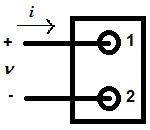
\includegraphics[scale=0.75]{elemento_basico_ideal}
	              \caption{Elemento básico ideal}
	          \end{figure}
	
	          \subsection{Potência elétrica instantânea}
	             
	             \begin{definition}[Potência elétrica instantânea]
	             É a taxa de variação de energia elétrica em um determinado tempo e, sua parte ativa, é medida em $Watt (W)$ no $SI$.
	             \begin{equation}
	             p(t) = \frac{d\omega}{dt} 
	             \end{equation}
	             Onde $p$ é a potência, $d\omega$ o elemento diferencial de energia e $dt$ o elemento diferencial de tempo.
	             Pela regra da cadeia, temos:
	             \begin{equation}\label{potencia}
	             p(t) = \frac{d\omega}{dt} = \frac{d\omega}{dq}\frac{dq}{dt} = v(t)i(t)
	             \end{equation}
	             
	             \end{definition}
	             
	    \section{Polaridades de referência e expressões de potência para um elemento básico ideal}
	        
	        \begin{figure*}[h]
    \centering
    \begin{subfigure}{0.5\textwidth}
        \centering
        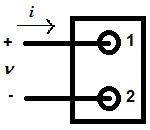
\includegraphics[scale=1]{elemento_basico_ideal}
        \caption{$p = vi$}
    \end{subfigure}%
    \begin{subfigure}{0.5\textwidth}
        \centering
        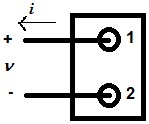
\includegraphics[scale=1]{elemento_basico_ideal1}
        \caption{$p = v(-i)$}
    \end{subfigure}
    ~ 
    \begin{subfigure}[t]{0.5\textwidth}
        \centering
        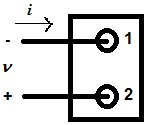
\includegraphics[scale=1]{elemento_basico_ideal2}
        \caption{$p = (-v)i$}
    \end{subfigure}%
    \begin{subfigure}[t]{0.5\textwidth}
        \centering
        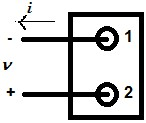
\includegraphics[scale=1]{elemento_basico_ideal3}
        \caption{$p = (-v)(-i)$}
    \end{subfigure}
    \caption{Polaridade}
\end{figure*}
	
	
	
%----------------------------------------------------------------------------------------
%	CHAPTER 2
%----------------------------------------------------------------------------------------
	
	\chapterimage{includes/documents/chapter_head_2.pdf} % Chapter heading image
	
	\chapter{Fontes de tensão e corrente}
	    
	    \section{Definição}
	        
	        \subsection{Fonte de tensão ideal independente}
	        
	        \begin{definition}
	            Uma fonte de \textbf{tensão} ideal independente mantém uma diferença de potencial em seus terminais independente da carga instalada.
	        \end{definition}
	        
	        \subsection{Fonte de corrente ideal independente}
	        
	        \begin{definition}
	            Uma fonte de \textbf{corrente} ideal independente mantém uma corrente em seu ramo independente da carga instalada.
	        \end{definition}
	        
	        \subsection{Fonte ideal dependente}
	        
	        \begin{definition}
	        Uma fonte dependente, ou controlada, seja esta de corrente ou tensão, consiste em uma fonte com algum parâmetro dado em função de outra grandeza.
	        \end{definition}        
	        
	    \section{Representação}
	    
	    \begin{table}[h]
	    \centering
	    \begin{tabular}{c c}
	    \toprule
	    Fontes independentes  & Fontes dependentes\\
	    \midrule
	    \begin{circuitikz}
	        \draw (0,0) to [V, v =$v$] (0,2) 
	              (2,0) to [I, i =$i$] (2,2);
	    \end{circuitikz}  & 
	    \begin{circuitikz}
	        \draw (2,0) to [cV, v =$\mu v_x$] (2,2)
	              (4,0) to [cV, v =$\rho i_x$] (4,2)
	              (6,0) to [cI, i =$\alpha v_x$] (6,2)
	              (8,0) to [cI, i =$\beta i_x$] (8,2);
	    \end{circuitikz}\\
	    \bottomrule
	    \end{tabular}
	    
	    \end{table}
	
	    
	    \section{Associação de fontes}
	    
	    A associação entre fontes deve ser feita de forma que as Leis de Kirchhoff sejam respeitadas. Desta forma, duas fontes de tensão associadas em paralelo precisam, necessariamente, ter a mesma amplitude e polaridade em qualquer instante. Fontes de corrente ligadas em série devem ter a mesma amplitude e sentido de corrente para que se torne possível a associação.
	    
	    \subsection{Exemplos de ligações permissíveis}

	    \begin{figure}[h!]\begin{center}       	    
	    \begin{circuitikz}
	        \draw (0,0) to [V, v =$v_1$] (0,2)
	              (0,2) to [V, v =$v_2$] (2,2)
	              (2,2) to [V, v =$v_3$] (4,2) 
	              (4,2) to[generic] (4,0)
	              (4,0) to (0,0);
	              
	    \end{circuitikz}\caption{Permissível para quaisquer valores de $v_1$, $v_2$ ou $v_3$}\end{center} 
	    \end{figure}
	    \begin{figure}[h!]\begin{center}       	    
	    \begin{circuitikz}
	        \draw (0,0) to [V, v =$v_1$] (0,2)
	              (0,2) to [V, v =$v_2$] (2,2)
	              (2,2) to [V, v =$v_3$] (4,2) 
	              (4,2) to [V, v =$v_4$] (4,0)
	              (4,0) to [V, v =$v_5$] (0,0);
	              
	    \end{circuitikz}\caption{Permissível se $\sum\limits_{\alpha = 1}^{5}v_\alpha = 0 $}\end{center} 
	    \end{figure}
	    \begin{figure}[h!]\begin{center}    
	    \begin{circuitikz}
	        \draw (0,0) to [I, i =$i_1$] (0,2)
	              (0,2) to (2,2)
	              (2,2) to [I, i =$i_2$] (2,0) 
	              (4,0) to [I, i =$i_3$] (4,2)
	              (2,2) to (4,2)
	              (4,0) to (0,0)
	              (4,2) to (6,2)
	              (4,0) to (6,0)
	              (6,0) to[generic] (6,2);
	              
	    \end{circuitikz}\caption{Permissível para quaisquer valores de $i_1$, $i_2$ ou $i_3$}\end{center} 
	    \end{figure}

	    \subsection{Exemplos de ligações não permissíveis}
	    
	    \begin{figure}[h!]\begin{center}    
	    
	    \begin{circuitikz}
	        \draw (0,0) to [V, v =$v_1$] (0,2)
	              (0,2) to (2,2)
	              (2,2) to [V, v =$v_1$] (2,0) 
	              (2,2) to (4,2)
	              (4,0) to (0,0)
	              
	              (4,0) to[generic] (4,2);
	              
	    \end{circuitikz}\caption{Não permissível} 
	       
	    \begin{circuitikz}
	        \draw (0,0) to [I, i =$i_1$] (0,2)
	              (2,2) to [I, i =$i_1$] (0,2)
	              (2,2) to [generic] (2,0)
	              (0,0) to (2,0);
	              
	    \end{circuitikz}\caption{Não permissível}\end{center} 
	    \end{figure}
	    
	    
%----------------------------------------------------------------------------------------
%	CHAPTER 3
%----------------------------------------------------------------------------------------
	
	\chapterimage{includes/documents/chapter_head_2.pdf} % Chapter heading image
	\chapter{Resistência elétrica e Lei de Ohm}
	
	    \section{Resistência elétrica}
	    
	        \subsection{Definição}
	            \begin{definition}[Resistência elétrica]
	                É a propriedade dos materiais de se opor à circulação de cargas elétricas.
	             \end{definition}
	         
	          A resistência elétrica dos materiais pode variar com a temperatura, com energia luminosa, e com outras propriedades do material, tais como área de secção transversal, comprimento e a resistividade. A resistividade corresponde à resistência elétrica que uma unidade de volume de material oferece ao fluxo de cargas e é própria de cada material. A resistência é medida em $Ohm (\Omega)$ e pode ser calculada em função do comprimento $l (m)$, da resistividade $\rho (\Omega m)$ e da área do material $A (m^2)$ da forma que segue:
	         
	                 \begin{equation}\label{oms2}
	                 R = \frac{\rho l}{A}
	                 \end{equation}
	            
	        \subsection{Resistor}
	      Um resistor é um componente eletrônico que tem por finalidade oferecer oposição à passagem de uma corrente. Por ser um elemento que não acumula energia, toda a potência entregue a este tipo de componente é dissipada em forma de calor, como é descrito pelo $efeito$ $Joule$. Esta propriedade permite a utilização de resistores na conversão de energia elétrica em energia térmica.
	        
	        \begin{figure}[!htbp]
    
    \centering
    \begin{subfigure}{0.5\textwidth}
        \centering
        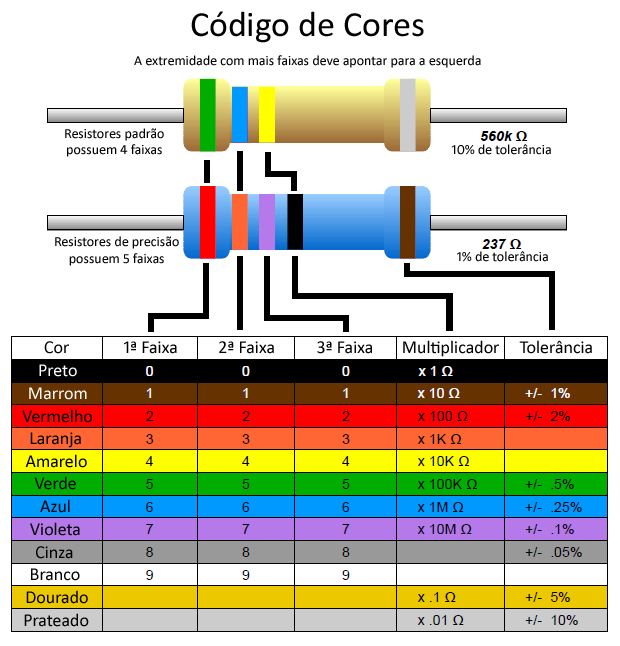
\includegraphics[scale=0.35]{codigo_de_cores}
        \caption{Código de cores para o valor da resistência}
    \end{subfigure}
    ~
    \begin{subfigure}{0.5\textwidth}
        \centering
        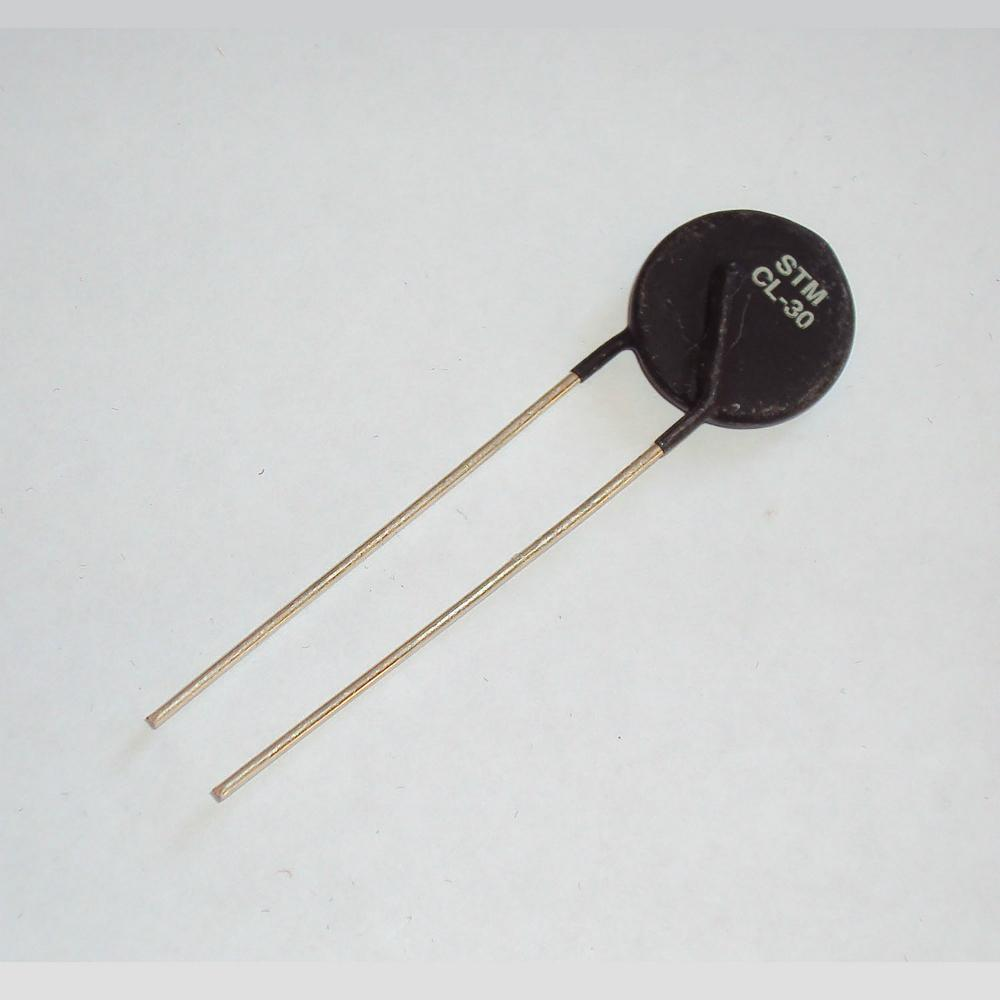
\includegraphics[scale=0.15]{Termistor}
        \caption{Termistor(Sensor de temperatura)}
    \end{subfigure}
    
    \begin{subfigure}{0.5\textwidth}
        \raggedright
        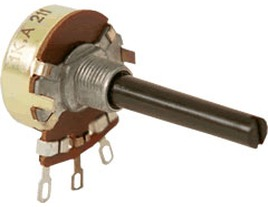
\includegraphics[scale=0.2]{Potenciometro}
        \caption{Potenciômetro (resistência como função do ângulo de deslocamento do eixo)}
    \end{subfigure}%
    \begin{subfigure}{0.5\textwidth}
        \raggedleft
        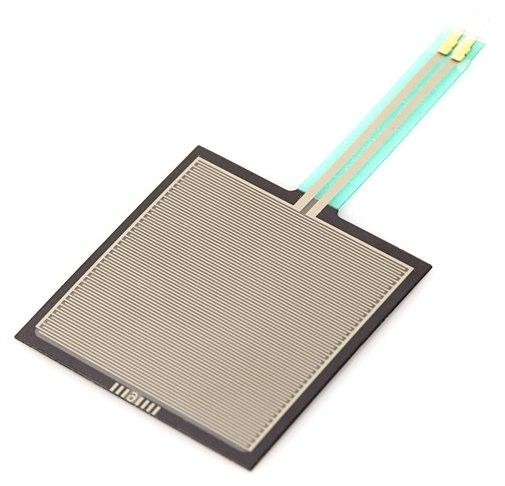
\includegraphics[scale=0.2]{Sensor_forca}
        \caption{Sensor de força quadrado}
    \end{subfigure}
    \begin{subfigure}{0.5\textwidth}
        \centering
        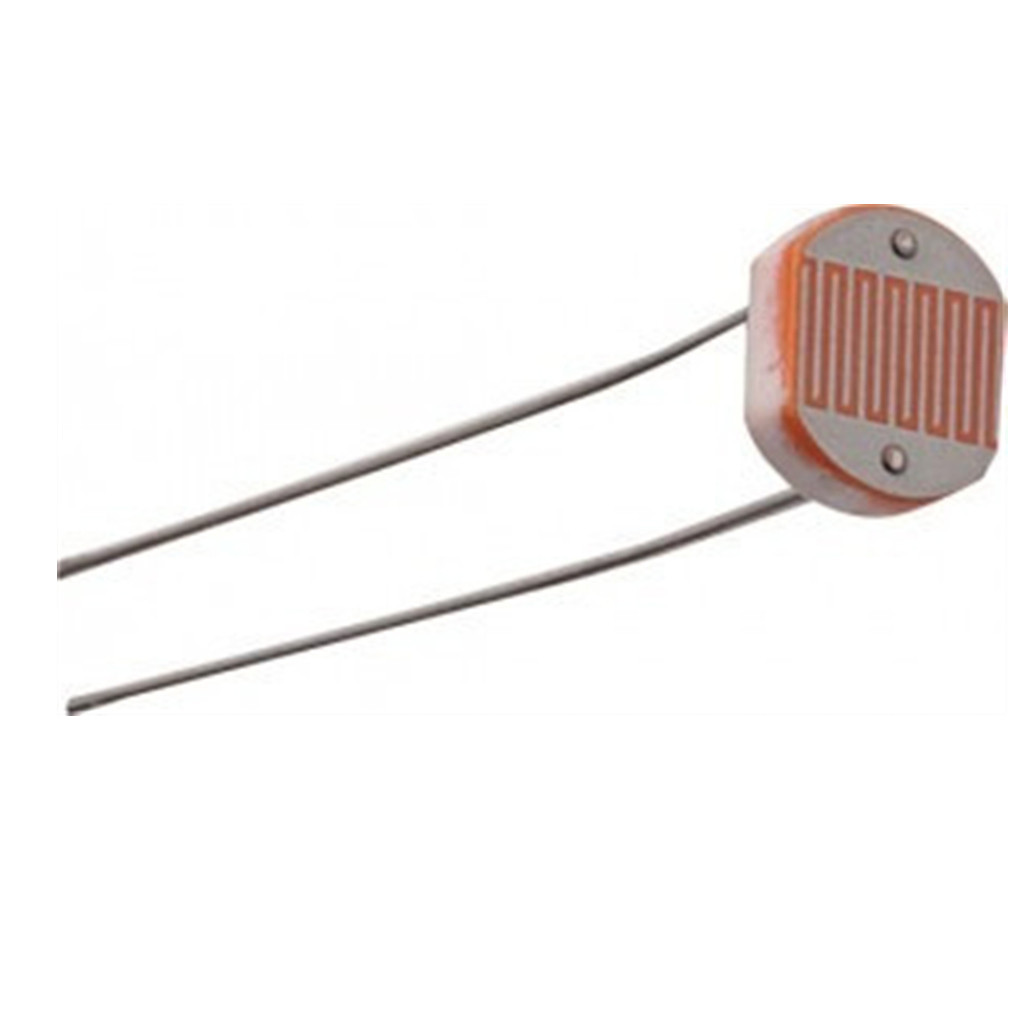
\includegraphics[scale=0.15]{LDR}
        \caption{LDR (Sensor de luminosidade)}
    \end{subfigure}%
    \begin{subfigure}[!htb]{0.5\textwidth}
        \centering
        \begin{circuitikz}[scale=3]
	            \draw (0,0) to [R=$R$] (2,0);
	            \end{circuitikz}
        \caption{Símbolo segundo a norma americana}
    \end{subfigure}
    \caption{Aspecto físico de componentes resistivos}\label{aspecto}
\end{figure}

Resistores, devido às propriedades dos materiais de variar a resistência em função de outras grandezas, podem ser utilizados na construção de sensores, como no caso dos termistores, dos Light Dependent Resistors (LDR's) e alguns sensores de força. Na figura \ref{aspecto} é possível observar alguns tipos de resistores e seu símbolo de acordo com a norma americana.
	   
     \section{Lei de Ohm}
     O físico alemão George Simon Ohm descobriu uma relação constante entre a tensão nos terminais de alguns elementos condutores e a corrente que por ele circula. Aos materiais que tendiam a manter esta proporcionalidade com alguma variação de temperatura foi dado o nome de resistores ohmicos. Além da relação estabelecida na equação \ref{oms2}, a Lei de Ohm estabelece que:
     \begin{equation}
         v = Ri
     \end{equation}
    
     Onde $v (V)$ é a tensão nos terminais do resistor, $ R(\Omega)$ a resistência elétrica e $i (A)$ a corrente elétrica que passa em seu ramo. Com esta relação linear, aumentar a corrente implica em um aumento de tensão e, consequentemente, um aumento na potência e no consumo de energia.
     \begin{remark}
      Resistores ideais não acumulam energia.
     \end{remark}
     
      Como resistores não acumulam nem podem fornecer energia, sua potência tende sempre a ser positiva, indicando consumo. Com isso, o sentido associado de corrente e tensão para esse tipo de elemento estabelece que a corrente que circula precisa, necessariamente, ter o mesmo sentido da queda de tensão.     
         
         \subsection{Cálculo de potência}	   
	  
	  Dado pela equação \ref{potencia}, a potencia de um resistor, instantaneamente, passa a ser:
	  \begin{equation}
	  p = Ri^2
	  \end{equation}
	  
	  Sendo a condutância, $G$, medida em Simens$(\mho)$ e dada pelo inverso da resistência, a potência instantânea no resistor pode ser calculada como:
	  \begin{equation}
	  p = \frac{v^2}{R} = Gv^2
	  \end{equation}
	  
	  
%----------------------------------------------------------------------------------------
%	CHAPTER 4
%----------------------------------------------------------------------------------------
	
\chapterimage{includes/documents/chapter_head_2.pdf} % Chapter heading image
\chapter{Leis de Kirchhoff}
    
    \section{Definições}
        
        \begin{definition}[Circuito planar]
        Circuito que pode ser desenhado em um plano sem que dois ou mais ramos se cruzem.
        \end{definition}
        \begin{definition}[Nó]
        Ponto de conexão entre dois ou mais terminais de elementos do circuito.
        \end{definition}
        \begin{definition}[Nó essencial]
        Ponto de conexão entre três ou mais terminais de elementos do circuito.
        \end{definition}
        \begin{definition}[Caminho]
        Sequencia de elementos ligados entre si sem que algum elemento seja incluído mais de uma vez.
        \end{definition}
        \begin{definition}[Ramo]
        Caminho que liga dois nós.
        \end{definition}
        \begin{definition}[Ramo essencial]
        Caminho qu liga dois nós essenciais.
        \end{definition}
        \begin{definition}[Malha]
        Caminho fechado cujo último nó coincide com o primeiro.
        \end{definition}
        \begin{definition}[Malha simples]
        Malha que não inclui outra malha.
        \end{definition}
        
    
    \section{Lei de Kirchhoff das tensões[LKT]}
    
    A lei de Kirchhof das tensões se baseia no fato do campo elétrico apresentar característica irrotacional, ou seja, representa um sistema conservativo. Isso implica que a circulação do campo elétrico seja nula.
    
    Sendo assim, a lei de Kirchhoff das tensões é anunciada da forma que segue:

\begin{definition}[LKT]
A soma algébrica das tensões em qualquer malha de um circuito é sempre nula.
\end{definition}    

Para sistematizar a análise, são indicadas as seguintes convenções no somatório das tensões:

\begin{remark}
 Queda de tensão positiva (+) e aumento de tensão negativa(-).
\end{remark}

\begin{remark}
Queda e tensão negativa (-) e aumento de tensão positiva (+).
\end{remark}

\begin{remark}
A utilização da convenção escolhida deve ser aplicada a todo o circuito, sendo proibida a utilização de forma aleatória para cada elemento.
\end{remark}
    
    \section{Lei de Kirchhoff das correntes[LKC]}
    
    A lei de Kirchhoff das correntes se baseia no princípio de conservação da carga, que estabelece que cargas elétricas não podem ser criadas ou destruídas, implicando que toda carga elétrica que "entre" em algum nó precisa, necessariamente, "sair" para que a quantidade líquida de cargas no circuito fechado permaneça constante.
    
    Por tanto, a lei de Kirchhoff das correntes estabelece que:
    
    \begin{definition}[LKT]
    A soma algébrica das correntes em qualquer nó do circuito é sempre nula.
    \end{definition}
    
    De forma análoga à LKT, a convenção para a análise se estabelece como segue:
    
    \begin{remark}
 Corrente que entra no nó (+) e corrente que sai do nó (-).
    \end{remark}

    \begin{remark}
 Corrente que entra no nó (-) e corrente que sai do nó (+).
    \end{remark}

    \begin{remark}
A utilização da convenção escolhida deve ser aplicada a todo o circuito, sendo proibida a utilização de forma aleatória para cada elemento.
    \end{remark}
    
    \section{Uso das leis de Kirchhoff e Ohm}
    
    A utilização das leis de Kirchhoff, e da lei de Ohm, possibilitam a modelagem de circuitos elétricos resistivos, por meio de equações lineares, que descrevem o comportamento das grandezas de tensão e corrente no circuito.
    
    Para modelar o circuito de maneira eficiente, é necessário, a priori, determinar o sentido das correntes nos ramos dos circuitos e as polaridades das tensões no elementos. Apesar das escolhas destas poderem ser arbitrárias, a utilização de convenções como, por exemplo, o sentido associado de tensão e corrente em resistores, podem reduzir os passos necessários à analise.
    
    \begin{example}[LKC]
        \begin{figure}[!htbp]
           \centering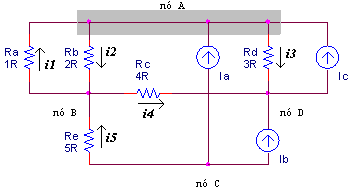
\includegraphics[scale=1]{exemploLKC}
            \caption{Análise dos nós}\label{LKCimg}  
        \end{figure}
                       
    
    Aplicando a LKC no circuito da imagem \ref{LKCimg} nos nós A, B, C e D, com a convenção de corrente entrando no nó positiva, temos:
    
    \begin{equation}\label{sistemaNo}
    \left\{\begin{aligned} & 
         \text{nó A:} && i_1 - i_2 + i_a - i_3 + i_c = 0\\& 
         \text{nó B:} && -i_1+i_2-i_4+i_5=0\\&
        \text{nó C:} && -i_5-i_a-i_b=0\\&
        \text{nó D:} && i_3+i_4+i_b-i_c=0
    \end{aligned}\right.
    \end{equation}
    \end{example}
    
    É possível observar que qualquer equação do sistema \ref{sistemaNo} pode ser obtida por combinações lineares das outras três.    
    \begin{example}[Equação do nó D dado por combinações lineares]
    $$ (-1)(i_1 - i_2 + i_a - i_3 + i_c) + (-1)(-i_1+i_2-i_4+i_5) + (-1)(-i_5-i_a-i_b)= i_3+i_4+i_b-i_c = 0 $$
    \end{example}
    
    
    \begin{example}[LKT]
        \begin{figure}[!htbp] \centering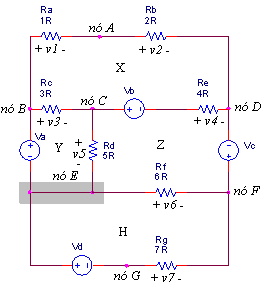
\includegraphics[scale=1]{exemploLKT}
            \caption{Análise das malhas}\label{LKTimg} 
        \end{figure} 
        
Aplicando a LKT no circuito da imagem \ref{LKTimg} nas malhas X, Y, Z e H, com a convenção de queda de tensão positiva no sentido horário, temos:    
    
\begin{equation}\label{sistemaMalha}
    \left\{\begin{aligned} & 
         \text{malha X:} && v_1+v_2-v_4-v_b-v_3=0\\& 
         \text{malha Y:} && v_3+v_5-v_a=0\\&
        \text{malha Z:} && v_b+v_4-v_c-v_6-v_5=0\\&
        \text{malha H:} && v_6-v_7-v_d=0
    \end{aligned}\right.
    \end{equation}    
    
 As quatro equações obtidas são linearmente independentes por todas as malhas analisadas serem malhas simples.    
    
    \end{example}
    
    \begin{example}[LKC e LKT]
    
        \begin{figure}[!htbp]               
            \centering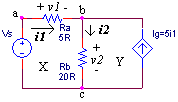
\includegraphics[scale=1]{exemploLKCT}
            \caption{Análise das malhas e nós}\label{LKCTimg} 
        \end{figure}
    
 Aplicando a LKT nas malhas X, Y e a LKC no nó b do circuito da figura \ref{LKCTimg}, temos:    
    
\begin{equation}
\text{nó b: } i_1-i_2+i_g=0
\end{equation}    

    Utilizando a relação definida pela fonte dependente, temos

\begin{equation}
i_1-i_2+5i_1 = 6i_1-i_2=0
\end{equation}    
    
\begin{equation}
\text{malha X: } v_1+v_2-v_s=0
\end{equation}  
    
Aplicando a lei de Ohm, temos:    
    
\begin{equation}
\text{malha X: } v_s=v_1+v_2=5i_1+20i_2
\end{equation}    
    
Dessa forma, obtém-se um sistema com duas equações para determinação das duas incógnitas $i_1$ e $i_2$:    
 
    \begin{equation}\label{sistemaMalhaNo}
    \left\{\begin{aligned} & 
          6i_1-i_2=0\\& 
 5i_1+20i_2=v_s
    \end{aligned}\right.
    \end{equation} 
    
Onde $v_s$ é um termo conhecido.    
    
    \end{example}

%----------------------------------------------------------------------------------------
%	CHAPTER 5
%----------------------------------------------------------------------------------------
	
\chapterimage{includes/documents/chapter_head_2.pdf} % Chapter heading image
\chapter{Circuitos resistivos simples}

\section{Ligação em série}
        
         \begin{figure}[!htbp] \centering
 \begin{circuitikz}[scale=1]
     \draw
         (0,2) to[R=$R_1$, v=$v_{R_1}$,i>=$i_1$] (2,2) 
               to[R=$R_2$, v=$v_{R_2}$,i>=$i_2$] (4,2)
               to[R=$R_3$, v=$v_{R_3}$,i>=$i_3$] (6,2)
               to[R,l_=$R_4$, v^=$v_{R_4}$,i>=$i_4$] (6,0) 
               to[R=$R_5$, v=$v_{R_5}$,i>=$i_5$] (4,0)
               to[R=$R_6$, v=$v_{R_6}$,i>=$i_6$] (2,0)               
               to[R=$R_7$, v=$v_{R_7}$,i>=$i_8$] (0,0)
         (0,0) to[V>=$v$, i>=$i_8$] (0,2)
         ;
 \end{circuitikz}
            \caption{Circuito resistivo em série}\label{capacitorSerie} 
        \end{figure}

 No circuito contido na figura \ref{Rserie}, é possível observar que um dos terminais da fonte de tensão $v_s$ está conectado a um terminal do resistor $R_1$. Em sequencia, o outro terminal do resistor $R_1$ se conecta a um terminal do resistor $R_2$, seguindo este padrão de ligação até que o segundo terminal do resistor $R_7$ se conecte ao segundo terminal da fonte de tensão.
 
 A ligação em série se caracteriza pela conexão em um nó de apenas dois elementos. Ao analisar as correntes do circuito em cada nó com a LKC, observa-se que:
 \begin{equation}
 i_1=i_8,i_2=i_1,i_3=i_2,i_4=i_3,i_5=i_4,i_6=i_5,i_7=i_6  $ e $ i_8=i_7
 \end{equation}
 
 
 Logo, conclui-se que:
 \begin{equation}
 i_1=i_2=i_3=i_4=i_5=i_6=i_7=i_8=i
 \end{equation}
 
 
 Ao aplicar a LKT, adotando o sentido horário e a queda de tensão positiva, tem:
 
 \begin{equation}
 -v_s+v_1+v_2+v_3+v_4+v_5+v_6+v_7=0
 \end{equation}

Logo:

\begin{equation}
 v_1+v_2+v_3+v_4+v_5+v_6+v_7=v_s
 \end{equation}
 
Pela lei de Ohm, vem:

\begin{equation}
v_s=R_1 i+R_2 i+R_3 i+R_4 i+R_5 i+R_6 i+R_7 i
\end{equation}

Observa-se que a tensão da fonte é dividida entre os componentes de forma proporcional ao valor de cada resistência. 
Com a corrente em evidência, vem:

\begin{equation}\label{eqRserie}
v_s= i(R_1+R_2+R_3+R_4+R_5+R_6+R_7)
\end{equation}

 \begin{figure}[!htbp]
\centering
    \begin{subfigure}{0.5\textwidth}
        \centering
        \begin{circuitikz}[scale=1]
	            \draw 
                (0,2) to[R=$R_1$, v=$v_{R_1}$,i>=$i_1$] (2,2) 
               to[R=$R_2$, v=$v_{R_2}$,i>=$i_2$] (4,2)
               to[R=$R_3$, v=$v_{R_3}$,i>=$i_3$] (6,2)
               to[R,l_=$R_4$, v^=$v_{R_4}$,i>=$i_4$] (6,0) 
               to[R=$R_5$, v=$v_{R_5}$,i>=$i_5$] (4,0)
               to[R=$R_6$, v=$v_{R_6}$,i>=$i_6$] (2,0)               
               to[R=$R_7$, v=$v_{R_7}$,i>=$i_8$] (0,0)
         (0,0) to[V>=$v_s$, i>=$i_8$] (0,2)
                             
	            ;
	     \end{circuitikz}
        \caption{Circuito no domínio do tempo}
    \end{subfigure}%
    \begin{subfigure}{0.5\textwidth}
        \centering
        \begin{circuitikz}[scale=1]
	            \draw 
                (0,0)to[V=$v_s$](0,2)to[short,i=$i$](2,2)to[R=$R_{eq}$](2,0)to(0,0)
                             
	            ;
	     \end{circuitikz}
        \caption{Circuito equivalente}\label{rEquivalente}
    \end{subfigure}
    \caption{Circuito representado no domínio do tempo e da frequência}
    \end{figure}
            

A equação \ref{eqRserie} sugere que, se o circuito for representado por apenas um resistor com resistência \textbf{equivalente} à soma de todos os componentes resistivos em série, neste circuito circulará uma corrente $i$ \textbf{igual} à corrente do circuito série original, quando o mesmo é alimentado pela mesma fonte de tensão $v_s$, como está representado na figura \ref{rEquivalente}.

De maneira geral, é possível afirmar que, em qualquer ligação em série com $n$ resistores, $R_{eq} = \sum\limits_{\alpha = 1}^{n}R_\alpha$

\begin{remark}
 Um circuito série pode ser caracterizado como um circuito em que a corrente que atravessa todos os elementos é exatamente a mesma em amplitude e sentido.
\end{remark}

\begin{remark}
Numa associação série de resistores, o resistor equivalente $R_{eq}$ será sempre maior que o maior dos resistores conectados em série.
\end{remark}

\section{Circuito divisor de tensão}

Como observado no circuito resistivo série, a tensão da fonte é dividida entre os elementos do circuito. Desta forma, este tipo de circuito pode ser classificado como \textbf{circuito divisor de tensão}. Para isto, a corrente que circula pelos elementos deve ser a mesma.

Para determinar a tensão em algum dos resistores não se faz necessário conhecer o valor da corrente que por ele circula, sabendo o valor de tensão da fonte e da resistência do resistor.

        \begin{figure}[!htbp] \centering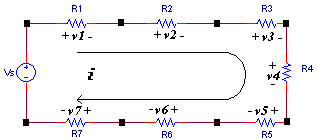
\includegraphics[scale=1]{divisorTensao}
            \caption{Circuito resistivo em série}\label{divisorTensao} 
        \end{figure}
        
Considerando o circuito da figura \ref{divisorTensao}, é possível determinar a corrente que circula entre os componentes da forma que segue:

\begin{equation}
i = \frac{v_s}{R_1+R_2+R_3+R_4+R_5+R_6+R_7}
\end{equation}

Para determinar o valor da tensão no resistor $R_1$, basta usar a lei de Ohm.

\begin{equation}
v_1 = R_1i = R_1\frac{v_s}{R_1+R_2+R_3+R_4+R_5+R_6+R_7}
\end{equation}

De maneira geral, a tensão em qualquer resistor da ligação pode ser dado por:

\begin{equation}
v_\alpha = \frac{R_\alpha}{R_1+R_2+R_3+R_4+R_5+R_6+R_7}v_s
\end{equation}
Onde $\alpha \in \mathbb{N} | \alpha \leq 7$

Para uma associação com $n$ resistores:

\begin{equation}
v_\alpha = \frac{R_\alpha}{\sum\limits_{\beta = 1}^{n}R_\beta}v_s
\end{equation}

\section{Ligação em paralelo}


        \begin{figure}[!htbp] \centering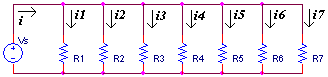
\includegraphics[scale=1]{circuitoRparalelo}
            \caption{Circuito resistivo em paralelo}\label{circuitoRparalelo} 
        \end{figure}

No circuito da figura \ref{circuitoRparalelo}, é possível observar que o padrão de ligações se dá de forma que um terminal da fonte de tensão compartilha o mesmo nó com um terminal de cada resistor do circuito. O padrão se repete para o segundo terminal. Isso faz com que todos os elementos do circuito estejam em paralelo.

A ligação em paralelo se caracteriza pelo compartilhamento de um mesmo par de nós entre os elementos. Este tipo de ligação faz com que a tensão seja a mesma em todos os elementos em paralelo. 

Analisando o circuito pela LKC, considerando a corrente entrando no nó positiva.

\begin{equation}
i-i_1-i_2-i_3-i_4-i_5-i_6-i_7=0
\end{equation}

logo:

\begin{equation}
i=i_1+i_2+i_3+i_4+i_5+i_6+i_7
\end{equation}

Pela lei de Ohm:

\begin{equation}\label{eqParalelo}
i= \frac{v_s}{R_1} + \frac{v_s}{R_2} +\frac{v_s}{R_3} +\frac{v_s}{R_4} +\frac{v_s}{R_5} +\frac{v_s}{R_6} +\frac{v_s}{R_7} 
\end{equation}

Pela equação \ref{eqParalelo}, é possível concluir que a corrente fornecida pela fonte é dividida entre as resistências de maneira proporcional ao inverso do seu valor.

Com a tensão $v_s$ em evidência, observa-se:

\begin{equation}\label{rEquivalenteParalelo}
i= v_s(\frac{1}{R_1} + \frac{1}{R_2} +\frac{1}{R_3} +\frac{1}{R_4} +\frac{1}{R_5} +\frac{1}{R_6} +\frac{1}{R_7})
\end{equation}

\begin{figure}[!htbp] \centering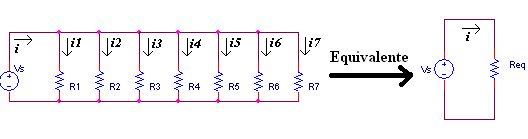
\includegraphics[scale=1]{rEquivalenteParalelo}
            \caption{Circuito resistivo em paralelo}\label{rEquivalenteParalelo} 
        \end{figure}

Pela equação \ref{circuitoRparalelo} sugere que, se o circuito for representado por apenas um resistor com condutância \textbf{equivalente} à soma das condutâncias dos resistores presentes no circuito, a corrente fornecida pela fonte de tensão será \textbf{igual} à corrente fornecida pela fonte de tensão no circuito original, como está representado na figura \ref{rEquivalenteParalelo}. Onde

\begin{equation}
\frac{1}{R_{eq}} = \frac{1}{R_1} + \frac{1}{R_2} +\frac{1}{R_3} +\frac{1}{R_4} +\frac{1}{R_5} +\frac{1}{R_6} +\frac{1}{R_7}
\end{equation}

De forma geral, pode se estabelecer que, para qualquer circuito resistivo com $n$ resistores em paralelo, tem:

\begin{equation}
\frac{1}{R_{eq}} = \sum\limits_{\alpha = 1}^{n} \frac{1}{R_\alpha}
\end{equation}

\begin{remark}
Um circuito paralelo pode ser caracterizado como um circuito em que a tensão aplicada aos terminais de todos os elementos é exatamente a mesma em amplitude e polaridade.
\end{remark}

\begin{remark}
Numa associação paralela de resistores, o resistor equivalente $R_{eq}$ será sempre menor do que o menor dos resistores conectados em paralelo. Essa afirmação pode ser confirmada pelo fato de que a condutância equivalente é maior do que a condutância individual de cada ramo resistivo do circuito, dado que a condutância equivalente é a soma dessas condutâncias individuais. Como maior condutância implica menor resistência, então confirma-se a afirmação inicial.
\end{remark}

\section{Circuito divisor de corrente}

Como observado no circuito resistivo paralelo, a corrente fornecida pela fonte de tensão é dividida entre os resistores da associação. Dessa forma, o circuito também pode ser denominado de \textbf{circuito divisor de corrente}. Deve-se observar que para isto ocorrer, a tensão entre os terminais de todos os elementos do circuito divisor de corrente deverá ser a mesma.

Para determinação da corrente em qualquer um dos resistores de um circuito paralelo (ou divisor de corrente), não é necessário conhecer a tensão aplicada aos resistores, bastando conhecer a corrente total e os valores de resistência, como será demonstrado a seguir.

        \begin{figure}[!htbp] \centering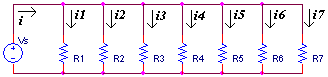
\includegraphics[scale=1]{divisorCorrente}
            \caption{Circuito resistivo em paralelo}\label{divisorCorrente} 
        \end{figure}

Considerando o circuito da figura \ref{divisorCorrente}, tem-se que a corrente total $i$ é dada por:

\begin{equation}
i= v_s(\frac{1}{R_1} + \frac{1}{R_2} +\frac{1}{R_3} +\frac{1}{R_4} +\frac{1}{R_5} +\frac{1}{R_6} +\frac{1}{R_7})
\end{equation}

Assim, para determinar a corrente no ramo de $R_1$, basta utilizar a lei de Ohm mais uma vez.

\begin{equation}
i = R_1i_1\frac{1}{R_1} + \frac{1}{R_2} +\frac{1}{R_3} +\frac{1}{R_4} +\frac{1}{R_5} +\frac{1}{R_6} +\frac{1}{R_7} \Rightarrow i_1 = \frac{i}{R_1(\frac{1}{R_1} + \frac{1}{R_2} +\frac{1}{R_3} +\frac{1}{R_4} +\frac{1}{R_5} +\frac{1}{R_6} +\frac{1}{R_7})}
\end{equation}

Em termos de condutância, tem:

\begin{equation}
i_1 = \frac{G_1}{G_1 + G_2 + G_3 + G_4 + G_5 + G_6 + G_7}i
\end{equation}

A generalização é trivial e cabe ao leitor.

\section{Ponte H}

\begin{figure}[!htbp]
    \centering
    \begin{circuitikz}
    \draw 
    (4,2) to[cspst=$CH_1$]  (4,4)
    (4,0) to[ospst=$CH_4$]  (4,2)
    (8,2) to[ospst=$CH_3$]  (8,4)
    (8,0) to[cspst=$CH_2$]  (8,2)
    (4,2) to[R=$R$, v=$v_R$](8,2)
    (4,0) to                (8,0)
    (4,4) to                (8,4)
    (0,0) to[V=$v_s$]       (0,4)
    (0,0) to                (4,0)
    (0,4) to                (4,4)
    ;
    \end{circuitikz}\caption{Ponte H}
    \label{ponteH}
\end{figure}

A ponte H consiste em uma topologia de circuito chaveado que permite a mudança de polaridade de tensão ou direção de corrente na carga instalada por meio da abertura e fechamento de chaves. Na imagem \ref{ponteH} é possível observar uma ponte H com uma carga resistiva.

\begin{figure}[!htbp]
    \centering
    \begin{circuitikz}
    \draw 
    (4,2) to                (4,4)    
    (8,0) to                (8,2)
    (4,2) to[R=$R$, v=$v_R$](8,2)
    (4,0) to                (8,0)
    (4,4) to                (8,4)
    (0,0) to[V=$v_s$]       (0,4)
    (0,0) to                (4,0)
    (0,4) to                (4,4)
    ;
    \end{circuitikz}\caption{$CH_1$ e $CH_2$ fechadas, e $CH_3$ e $CH_4$ abertas}
    \label{CH12}
\end{figure}

A figura \ref{CH12} representa a topologia do circuito quando as chaves $CH_1$ e $CH_2$ são fechadas, mantendo a tensão $v_s$ sobre o resistor $R$.

\begin{figure}[!htbp]
    \centering
    \begin{circuitikz}
    \draw 
    
    (4,0) to                (4,2)
    (8,2) to                (8,4)    
    (4,2) to[R=$R$, v=$v_R$](8,2)
    (4,0) to                (8,0)
    (4,4) to                (8,4)
    (0,0) to[V=$v_s$]       (0,4)
    (0,0) to                (4,0)
    (0,4) to                (4,4)
    ;
    \end{circuitikz}\caption{$CH_3$ e $CH_4$ fechadas, e $CH_1$ e $CH_2$ abertas}
    \label{CH34}
\end{figure}

A figura \ref{CH34} representa a topologia do circuito quando as chaves $CH_3$ e $CH_4$ são fechadas, mantendo a tensão $-v_s$ sobre o resistor $R$.

\section{Ponte de Wheatstone}
       \begin{figure}[!htbp] \centering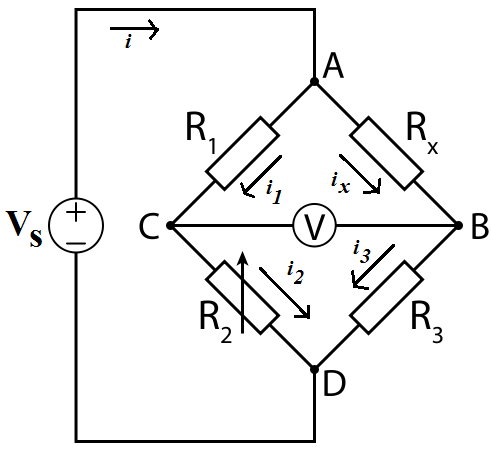
\includegraphics[scale=0.5]{ponteW}
            \caption{Ponte de Wheatstone}\label{ponteW} 
        \end{figure}

A ponte de Wheatstone, que tem sua topologia representada no circuito da figura \ref{ponteW}, é utilizada em alguns circuitos que tem por finalidade a medição de resistências. O princípio de operação deste circuito se baseia na condição de equilíbrio da ponte garantida pelos resistores $R_1$, $R_2$, $R_3$ e $R_x$ que, quando atingida, a diferença de potencial entre os nós $C$ e $B$ se anula.

Na condição de equilíbrio, segue:

$v_{CB} = 0 \Rightarrow v_{AC} = v_{AB} \text{, } v_{CD} = v_{BD} \text{, } i_1 = i_2 \text{, } i_x = i_3$

\begin{equation}
R_1i_1 = R_xi_x \text{ e }R_2i_2 = R_3i_3 
\end{equation}

\begin{equation}
\frac{R_1}{R_x} = \frac{i_x}{i_1} \text{ e } \frac{R_2}{R_3} = \frac{i_3}{i_2}
\end{equation}

\begin{equation}
\frac{i_x}{i_1} = \frac{i_3}{i_2} \Rightarrow \frac{R_1}{R_x} = \frac{R_2}{R_3}
\end{equation}

\begin{equation}
R_x = \frac{R_1R_3}{R_2}
\end{equation}

Relembrando que a resistência elétrica de alguns materiais pode variar com grandezas do meio, esta estrutura pode ser utilizada, com a utilização de sensores resistivos, para medir, de forma indireta, a luminosidade de um ambiente, a temperatura, pressão e etc. 

\section{Ligação $\Delta $-Y}

Na associação $\Delta - Y$ de resistores, não é possível aplicar os procedimentos de simplificação de circuitos resistivos, como os desenvolvidos para associação série ou paralela entre resistores de forma direta. Dependendo do tipo de associação estrela ou triângulo presente em um circuito, é possível realizar uma conversão estrela/triângulo, ou vice-versa, de modo a permitir uma análise mais simples do circuito. A transformação de uma associação estrela para triângulo deverá preservar o mesmo nível de corrente e tensão observados nos pontos de conexão da associação estrela ou triângulo original.

 \begin{figure}[!htbp] \centering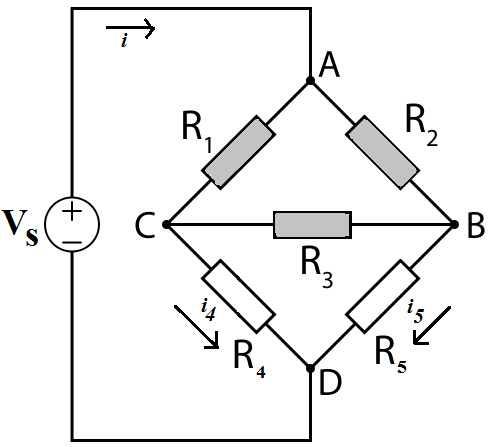
\includegraphics[scale=0.5]{ponteDeltaY}
            \caption{Ligação $\Delta$}\label{ponteDeltaY} 
        \end{figure}
        
Na figura \ref{ponteDeltaY}, está presente um circuito composto por cinco resistores no qual não é possível uma simplificação direta usando métodos de associação série ou paralela. Neste caso, uma possibilidade de obter um circuito simplificado é realizar uma transformação $\Delta - Y$, tomando os resistores $R_1$, $R_2$ e $R_3$, que estão conectados em $\Delta$. De modo a que o circuito obtido seja equivalente ao circuito original, é necessário que no circuito resultante as correntes $i$, $i_4$ e $i_5$ sejam as mesmas do circuito original, levando também a que as tensões $v_{AB}$, $v_{AC}$ e $v_{CB}$ também sejam as mesmas do circuito original.

 \begin{figure}[!htbp] \centering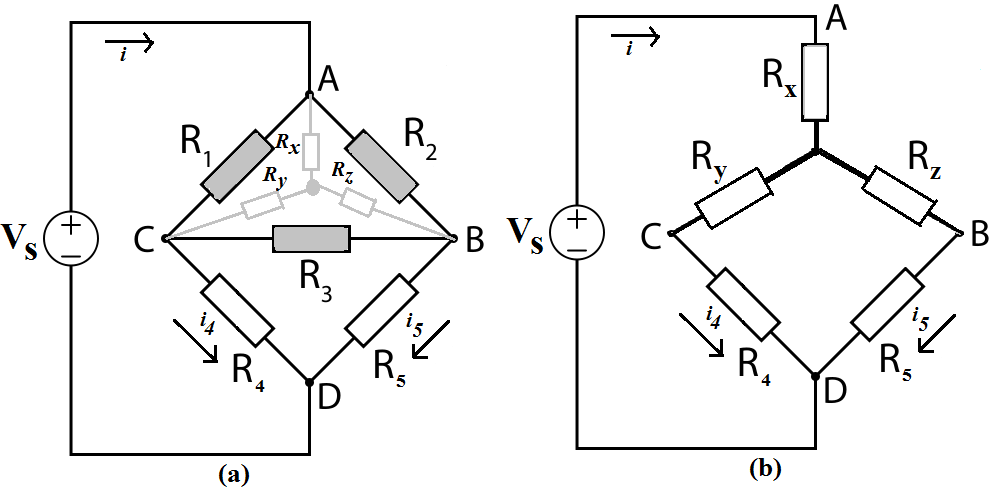
\includegraphics[scale=0.25]{ponteYab}
            \caption{Ligação $\Delta \Rightarrow Y$}\label{ponteYab} 
        \end{figure}

O circuito modificado, após a transformação $\Delta - Y$, é o representado na figura \ref{ponteYab}.

Observando o circuito da imagem \ref{ponteYab}, percebe-se que após a transformação $\Delta - Y$, o circuito equivalente resultante, formado pelos resistores $R_x$, $R_y$ e $R_z$, torna possível determinar uma resistência equivalente a qual será dada por $R_x+(R_y +R_4)$//$(R_z+R_5)$.

 
    \subsection{Determinação dos valores de resistências equivalentes}
        \subsubsection{$R_x$, $R_y$ e $R_z$}

        \begin{figure}[!htbp] \centering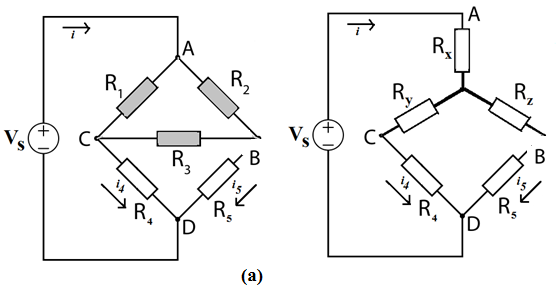
\includegraphics[scale=0.5]{ponteDeltaY2}
            \caption{}\label{ponteDeltaY2} 
        \end{figure}

Como discutido, o circuito formado pelos resistores $R_x$, $R_y$, $R_z$, $R_4$ e $R_5$, será equivalente ao circuito formado pelos resistores $R_1$, $R_2$, $R_3$, $R_4$ e $R_5$, se as tensões $v_{AC}$, $v_{AB}$, $v_{CB}$ e correntes $i$, $i_4$ e $i_5$, em ambos os circuitos forem as mesmas. Isso indica que as resistências equivalentes, vistas de qualquer um dos pares de terminais $AB$, $AC$ ou $BC$, como indicado na figura \ref{ponteDeltaY2}, de qualquer um dos circuitos, devem ser exatamente iguais.

\begin{equation}
R_{{eq}_{AC}}^{\Delta}=R_1//(R_2+R_3)=\frac{R_1 (R_2+R_3)}{R_1+R_2+R_3}
\end{equation}   

\begin{equation}
R_{{eq}_{AC}}^Y=R_x+R_y
\end{equation}  

\begin{equation}
R_{{eq}_{AC}}^Y=R_{{eq}_{AC}}^\Delta \Rightarrow R_x+R_y =\frac{R_1 (R_2+R_3)}{R_1+R_2+R_3}
\end{equation}   
        
\begin{equation}
R_{{eq}_{AB}}^{\Delta}=R_2//(R_1+R_3)=\frac{R_2 (R_1+R_3)}{R_1+R_2+R_3}
\end{equation}   

\begin{equation}
R_{{eq}_{AB}}^Y=R_x+R_z
\end{equation}  

\begin{equation}
R_{{eq}_{AB}}^Y=R_{{eq}_{AB}}^\Delta \Rightarrow R_x+R_z =\frac{R_2 (R_1+R_3)}{R_1+R_2+R_3}
\end{equation}

\begin{equation}
R_{{eq}_{BC}}^{\Delta}=R_3//(R_1+R_2)=\frac{R_3 (R_1+R_2)}{R_1+R_2+R_3}
\end{equation}   

\begin{equation}
R_{{eq}_{BC}}^Y=R_y+R_z
\end{equation}  

\begin{equation}
R_{{eq}_{BC}}^Y=R_{{eq}_{BC}}^\Delta \Rightarrow R_y+R_z =\frac{R_3 (R_1+R_2)}{R_1+R_2+R_3}
\end{equation}   

Desenvolvendo o conjunto das equações das resistências equivalentes para cada circuito, temos:

\begin{equation}\label{sistemaNo}
    \left\{\begin{aligned} & 
          R_y+R_z=\frac{R_3 (R_1+R_2)}{R_1+R_2+R_3}\\& 
          R_x+R_z=\frac{R_2 (R_1+R_3)}{R_1+R_2+R_3}\\&
          R_x+R_y=\frac{R_1 (R_2+R_3)}{R_1+R_2+R_3}
    \end{aligned}\right.
    \end{equation}
        
Considerando $R_1+R_2+R_3$, como $R_d$, multiplicando as duas primeiras equações por $-1$ e em seguida somando as mesmas, temos:

\begin{equation}
-R_y-R_z-R_x-R_z+R_x+R_y=\frac{-R_1 R_3-R_2 R_3-R_1 R_2-R_2 R_3+R_1 R_2+R_1 R_3}{R_d}
\end{equation}        

\begin{equation}
-2R_z=\frac{-2R_2 R_3}{R_d} \Rightarrow R_z=\frac{R_2 R_3}{R_1+R_2+R_3}
\end{equation}

De forma análoga,as operações lineares podem ser utilizadas na determinação de $R_x$ e $R_y$.

\begin{equation}
R_y=\frac{R_1 R_3}{R_1+R_2+R_3}
\end{equation}

\begin{equation}
 R_x=\frac{R_1 R_2}{R_1+R_2+R_3}
\end{equation}

\begin{remark}
A expressão para cada resistência equivalente da conexão $Y$ é obtida através de uma expressão que é função das resistências do circuito $\Delta$, onde o denominador é a soma de todas as resistências do circuito $\Delta$ e o numerador é o produto das duas resistências do circuito $\Delta$ adjacentes a resistência do circuito $Y$ que se deseja determinar.
\end{remark} 
 
 
        \subsubsection{$R_1$, $R_2$ e $R_3$}
        
        Na transformação $Y-\Delta$, dado o circuito original formado pelos resistores $R_x$, $R_y$, $R_z$, $R_4$ e $R_5$, um circuito equivalente formado pelos resistores $R_1$, $R_2$, $R_3$, $R_4$ e $R_5$, pode ser determinado. As considerações de equivalências discutidas na transformação $\Delta - Y$ são as mesmas, logo as expressões das resistências equivalentes entre os terminais $AB$, $AC$ e $BC$ são as mesmas.
        
 \begin{equation}
    \left\{\begin{aligned} & 
          R_y+R_z=\frac{R_3 (R_1+R_2)}{R_1+R_2+R_3}\\& 
          R_x+R_z=\frac{R_2 (R_1+R_3)}{R_1+R_2+R_3}\\&
          R_x+R_y=\frac{R_1 (R_2+R_3)}{R_1+R_2+R_3}
    \end{aligned}\right.
    \end{equation}
    
    Para determinação das expressões de $R_1$, $R_2$ e $R_3$ a partir de $R_x$, $R_y$ e $R_z$, devemos dividir as expressões entre si e aplicar as relações de transformação de $\Delta - Y$ previamente determinadas.
    
    Dividindo a expressão de $R_y+R_z$ pela expressão de $R_x+R_z$:
    
    \begin{equation}
    \frac{R_y+R_z}{R_x+R_z} = \frac{R_3 (R_1+R_2)}{R_2 (R_1+R_3)} \Rightarrow (R_y+R_z)R_2 (R_1+R_3 )=(R_x+R_z ) R_3 (R_1+R_2)
    \end{equation}
    
    \begin{equation}
    R_y R_1 R_2+R_z R_1 R_2+R_y R_2 R_3+R_z R_2 R_3=R_x R_1 R_3+R_z R_1 R_3+R_x R_2 R_3+R_z R_2 R_3
    \end{equation}
    
    Cancelando os dois últimos termos e observando que $R_1 R_2=R_x R_d$, $R_1 R_3=R_y R_d$ e $R_2 R_3=R_z R_d$, onde $R_d=R_1+R_2+R_3$, vem:
    
    \begin{equation}\label{eqanterior}
    R_y R_x R_d+R_z R_x R_d+R_y R_z R_d=R_x R_1 R_3+R_z R_1 R_3+R_x R_2 R_3
    \end{equation}
    
    Da expressão $R_x=\frac{R_1 R_2}{R_d}$, temos que $\frac{R_x}{R_1} = \frac{R_2}{R_d}$, assim, substituindo este resultado em $R_z=\frac{R_2 R_3}{R_d}$, $R_z=\frac{R_3 R_x}{R_1} \Rightarrow R_z R_1=R_x R_3$. Substituindo este resultado na equação \ref{eqanterior}:
    
    \begin{equation}
    R_y R_x R_d+R_z R_x R_d+R_y R_z R_d=R_x R_1 R_3+R_x R_3 R_3+R_x R_2 R_3
    \end{equation}
    
    Colocando o termo $R_xR_3$ em evidência:
    
    \begin{equation}
    R_y R_x R_d+R_z R_x R_d+R_y R_z R_d=R_x R_3 (R_1+R_3+R_2 )=R_x R_3 R_d
    \end{equation}
    
    Logo
    
    \begin{equation}
    R_3=\frac{R_x R_y+R_z R_x+R_y R_z}{R_x}
    \end{equation}
    
    De modo equivalente, as expressões para $R_1$ e $R_2$ podem ser determinadas.
    
    \begin{equation}
    \left\{\begin{aligned} & 
          R_1=\frac{R_x R_y+R_z R_x+R_y R_z}{R_z}\\& 
          R_2=\frac{R_x R_y+R_z R_x+R_y R_z}{R_y}\\&
          R_3=\frac{R_x R_y+R_z R_x+R_y R_z}{R_x}
    \end{aligned}\right.
    \end{equation}
    
    \begin{remark}
    A expressão para cada resistência equivalente da conexão $\Delta$ é obtida por meio de uma expressão que é função das resistências do circuito $Y$ na qual o denominador é igual a resistência do circuito $Y$ original, diametralmente oposta a resistência do circuito $\Delta$ que se deseja determinar e o numerador é a soma do produto dois a dois das resistências do circuito $Y$ original.
    \end{remark}
        
%----------------------------------------------------------------------------------------
%	CHAPTER 6
%----------------------------------------------------------------------------------------
	
\chapterimage{includes/documents/chapter_head_2.pdf} % Chapter heading image
\chapter{Técnicas de análise de circuitos}

\section{Consequencias da linearidade das leis de Kirchhoff}

\begin{itemize}
\item LKC – Circuito com $n$ nós possibilita obter $n-1$ equações linearmente independentes.
\item LKT – Obtém-se as $k$ outras equações independentes para determinar todas as incógnitas do circuito, onde $k=b-(n-1)$ e $b$ é o número de incógnitas.
\item O uso de nós essenciais diminui o número de incógnitas a determinar (número de nós essenciais, $n_e$ é menor ou igual ao número de nós, $n$, em um circuito).
\item Ao usar os nós essenciais para obtenção das equações de corrente, as demais $k$ equações necessárias para obter uma solução única podem ser definidas a partir das equações das malhas simples do circuito.
\item Em circuitos acoplados por fontes dependentes mantém a corrente no ramo de interligação das partes do circuito nula. A interligação mantém o mesmo potencial entre as partes do circuito, tomada com relação a um mesmo potencial de referência.
\item Circuitos acoplados por fontes dependentes: LKC fornece $n-s$ expressões de corrente independentes, onde $n$ é o número de nós e $s$ o número de partes.
\item Circuitos acoplados por fontes dependentes: LKT fornece $b-(n-s)$ expressões de malhas independentes, onde $b$ é o número de incógnitas.
\end{itemize}

\section{Técnica da tensão de nó}
        
 A técnica de análise da tensão de nó consiste na sistematização da solução do circuito utilizando a LKC e a lei de Ohm.
 
 Os passos necessários à modelagem dos circuitos com esta técnica são listados a seguir.

 \begin{enumerate}
 \item Desenhar o circuito sem cruzamento de ramos e identificar os nós essenciais.
 \item Selecionar um nó essencial como sendo o nó de referência. De preferência o nó que está conectado ao maior número de ramos.
 \item Definir as tensões de nó com relação ao nó de referência.
 \item Definir as correntes nos ramos e a convenção utilizada para corrente que entra e sai dos nós.
 \item Escrever as equações de corrente para os nós essenciais, com exceção do nó de referência.
 \item Escrever as equações obtidas como função da diferença de potencial entre os nós que estabelecem a ligação e da grandeza elétrica do componente presente no ramo.
 \end{enumerate}

\begin{example}[Aplicação]
\begin{figure}[!htbp] \centering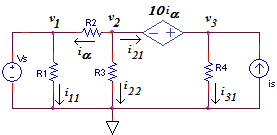
\includegraphics[scale=1]{tensaoNoEx}
            \caption{}\label{tensaoNoEx} 
        \end{figure}
        
Os passos do 1 ao 4 já foram realizados para a solução do circuito na figura \ref{tensaoNoEx}. Seguindo a sequencia:

Como o objetivo é determinar a tensão em cada nó essencial e, com estes, os valores das correntes nos ramos, é fácil observar que a tensão no nó $1$ em relação à referência é estabelecida pela fonte de tensão que mantém esse valor igual a $v_s$. Para os nós essenciais $2$ e $3$:

\begin{equation}\label{sistemaNo}
    \left\{\begin{aligned} & 
         \text{nó 2:} && i_\alpha + i_{22} + i_{21}=0\\& 
        \text{nó 3:} && -i_{21}+i_{31}-i_s=0
    \end{aligned}\right.
    \end{equation} 
    
    Pela lei de Ohm, os valores das correntes podem ser determinadas por:
    
    \begin{equation}\label{sistemaNo}
    \left\{\begin{aligned} & 
          i_\alpha = \frac{v_2-v_1}{R_2}\\& 
         i_{22}=\frac{v_2 - 0}{R_3}\\&
         i_{31} = \frac{v_3-0}{R_4}
    \end{aligned}\right.
    \end{equation} 
    
    \begin{equation}\label{sistemaNo}
    \left\{\begin{aligned} & 
         \text{nó 2:} && \frac{v_2-v_1}{R_2} + \frac{v_2}{R_3} + i_{21}=0\\& 
        \text{nó 3:} && -i_{21}+ \frac{v_3}{R_4}-i_s=0
    \end{aligned}\right.
    \end{equation}
    
    Agora é o momento de observar que a corrente $i_{21}$ não pode ser determinada. Porém, somando as equações dos nós $1$ e $2$, é possível eliminar o termo.
    
    \begin{equation}\label{superNo}
    \frac{v_2-v_1}{R_2} + \frac{v_2}{R_3}+\frac{v_3}{R_4}-i_s = 0
    \end{equation}
    
    Esta escolha, apesar de eliminar uma variável da equação, fornece uma só equação com duas variáveis. Outro fato que deve receber atenção é a fonte de tensão dependente fornecer uma relação entre as tensões nos nós $3$ e $2$.
    
    \begin{equation}
    v_3-v_2 = 10i_\alpha \Rightarrow v_3-v_2 = 10\frac{v_2-v_1}{R_2}
    \end{equation}
    
    Resultando, novamente, em um sistema com duas incógnitas e duas equações.
    
    \begin{equation}\label{sistemaNo}
    \left\{\begin{aligned} & 
          \frac{v_2-v_1}{R_2} + \frac{v_2}{R_3}+\frac{v_3}{R_4}-i_s = 0\\&
         v_3-v_2 = 10\frac{v_2-v_1}{R_2}
    \end{aligned}\right.
    \end{equation}
    
\begin{figure}[!htbp] \centering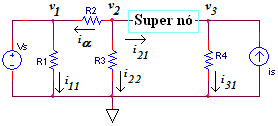
\includegraphics[scale=1]{superNoImg}
            \caption{}\label{superNoImg} 
        \end{figure}    
    
    A equação \ref{superNo} poderia ser obtida de forma direta tratando o ramo da fonte de tensão dependente como um super nó, como é descrito na imagem \ref{superNoImg}.
    \end{example}

\section{Técnica da corrente de malha}

O método das correntes de malha, que é baseado na LKT, tem como objetivo levar a solução da análise de um circuito, reduzindo o número de equações do sistema de equações que deve ser gerado para determinação do conjunto de grandezas de interesse.

\begin{remark}
A técnica das correntes de malha só podem ser aplicadas à circuitos planares.
\end{remark}

\begin{definition}[Corrente de malha]
Corrente hipotética que circula no perímetro de uma malha, podendo ou não coincidir com as correntes nos ramos.
\end{definition}

       \begin{figure}[!htbp] \centering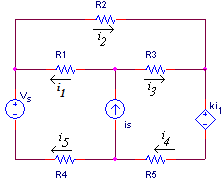
\includegraphics[scale=1]{correnteMalhaLKC}
            \caption{}\label{correnteMalhaLKC} 
        \end{figure} 
        \begin{figure}[!htbp] \centering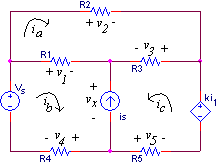
\includegraphics[scale=1]{correnteMalha}
            \caption{}\label{correnteMalha} 
        \end{figure} 

\begin{example}[]
Considerando que se deseja determinar as correntes $i_1$, $i_2$, $i_3$, $i_4$ e $i_5$ do circuito da figura \ref{correnteMalhaLKC}, pelos métodos convencionais (LKT, LKC, etc), seria necessário um sistema de cinco equações para se obter os valores das correntes. Aplicando o método das correntes de malha, define-se, para o circuito em questão, que possui três malhas simples, três correntes de malha, indicadas por $i_a$, $i_b$ e $i_c$, como mostrado na figura \ref{correnteMalha}. Inicialmente, podemos estabelecer a relação entre as correntes de malha $i_a$, $i_b$ e $i_c$ e as correntes a determinar (correntes de ramo) $i_1$, $i_2$, $i_3$, $i_4$  e $i_5$, sendo estas definidas por:

\begin{equation}\label{sistemaMalha}
    \left\{\begin{aligned} &           
         i_1=i_a-i_b\\&
i_2=i_a\\&
i_3=-(i_a+i_c)\\&
i_4=-i_c\\&
i_5=i_b
    \end{aligned}\right.
    \end{equation}

No circuito da figura \ref{correnteMalha}, percebe-se que os elementos $R_1$, $R_3$ e a fonte $i_s$ são compartilhados por mais de uma malha. No caso dos resistores, as polaridades de referência, indicadas no circuito, foram definidas considerando $i_b$, no caso de $R_1$ e no caso de $R_3$, tanto $i_a$ como $i_c$ foram consideradas, visto que ambas atravessam o referido resistor numa mesma direção. Utilizando a LKT e percorrendo as malhas no sentido de circulação das respectivas correntes de malha, considerando queda de tensão positiva, temos:

    \begin{equation}\label{sistemaNo}
     \left\{\begin{aligned} & 
        \text{malha de $i_a$: } && v_2+v_3-v_1=0\\& 
        \text{malha de $i_b$: } && -v_s+v_1+v_x+v_4=0\\& 
        \text{malha de $i_c$: } && v_x+v_3-ki_1+v_5=0
    \end{aligned}\right.
    \end{equation}
    
    Reescrevendo as equações de tensão em termos de correntes e resistências temos:
    
    \begin{equation}\label{sistemaMalha}
     \left\{\begin{aligned} & 
        \text{malha de $i_a$: } && R_2 i_a+R_3 (i_a+i_c )-R_1 (i_b-i_a )=0\\& 
        \text{malha de $i_b$: } && -v_s+R_1 (i_b-i_a )+v_x+R_4 i_b=0\\& 
        \text{malha de $i_c$: } && v_x+R_3 (i_a+i_c )-k(i_a-i_b )+R_5 i_c=0
    \end{aligned}\right.
    \end{equation}
    
    Observa-se nas equações \ref{sistemaMalha}, a existência do termo $v_x$ que não pode ser definido a partir de uma relação entre correntes de malha e resistência, visto que o mesmo representa a tensão sobre uma fonte de corrente. Subtraindo da equação de malha da corrente $i_b$, a expressão da equação de malha da corrente $i_c$ para eliminar o termo $v_x$, temos:

\begin{equation}\label{sistemaMalha}    
 \text{malha de $i_b$ - malha de $i_c$: } -v_s+R_1 (i_b-i_a )+R_4 i_b-R_3 (i_a+i_c )+k(i_a-i_b )-R_5 i_c=0 
\end{equation}

Para determinar de forma única os valores de $i_a$, $i_b$ e $i_c$, ainda falta uma equação. Esta, é definida pela relação estabelecida entre a fonte de corrente e as correntes de malha, cujas malhas compartilham a fonte de corrente, ou seja, no nesse exemplo, a fonte de corrente $i_s$ é compartilhada pelas malhas onde circulam as correntes de malha $i_b$ e $i_c$, assim, há uma relação entre estas corrente e a corrente da fonte definida por:

\begin{equation}
i_s=-(i_b+i_c )
\end{equation}

\begin{figure}[!htbp] \centering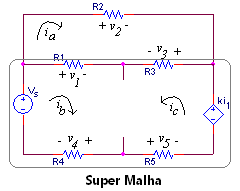
\includegraphics[scale=1]{superMalhaImg}
            \caption{}\label{superMalhaImg} 
        \end{figure}
    
A equação \ref{sistemaMalha} poderia ser obtida de forma direta se fosse eliminado o ramo onde está a fonte de corrente $i_s$, dessa forma, unindo as malhas simples onde circulam as correntes de malha $i_b$ e $i_c$. Esta malha resultante é denominada de "super malha" (ver figura \ref{superMalhaImg}). Sabendo que isto é apenas um artifício para obtenção de expressões sem a presença do termo $v_x$ e que as correntes de malha devem ser mantidas inalteradas.
\end{example}
\section{Transformação de fonte}

\begin{figure}[!htbp] \centering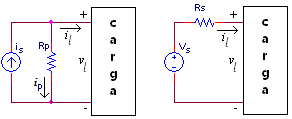
\includegraphics[scale=1]{transformacaoFonte}
            \caption{}\label{transformacaoFonte} 
        \end{figure}
        
Os circuitos na figura \ref{transformacaoFonte} podem ser considerados equivalentes, sendo alimentados por uma fonte de tensão em série com uma resistência ou por uma fonte de corrente em paralelo com uma resistência, se a tensão entre os terminais da carga, $v_l$, e a corrente de carga, $i_l$, forem iguais. Respeitando-se essas condições de equivalência, é então possível transformar um circuito que contenha uma fonte de tensão em série com um resistor em um circuito com uma fonte de corrente em paralelo com um resistor.

Considerando as premissas de equivalência acima indicadas e definindo que a resistência em série com a fonte de tensão, $R_s$, será igual a resistência a ser conectada em paralelo com a fonte de corrente, $R_p$, deve-se determinar uma expressão para $v_s$, a partir de $i_s$, na transformação fonte de corrente $\rightarrow$ fonte de tensão, bem como uma expressão para $i_s$, a partir de $v_s$, na transformação fonte de tensão $\rightarrow$ fonte de corrente.

Do circuito com a fonte de tensão, temos: $v_s=R_s i_l+v_l$. Do circuito com a fonte de corrente temos: $v_l=R_p i_p=R_p (i_s-i_l )$. Substituindo o valor de $v_l$ na primeira expressão, temos:

\begin{equation}
v_s=R_s i_l+R_p (i_s-i_l )
\end{equation} 

Como $R_s=R_p=R$, temos:

\begin{equation}
v_s=Ri_l+Ri_s-Ri_l=Ri_s
\end{equation}

Assim, na transformação fonte de corrente $\rightarrow$ fonte de tensão, teremos: $v_s=Ri_s$. Na transformação fonte de tensão $\rightarrow$ fonte de corrente, teremos: $i_s= \frac{v_s}{R}$.


\section{Circuito equivalente de Thévenin e Norton}
    
    \begin{theorem}[Teorema de Thévenin]
    Qualquer circuito linear invariante no tempo pode ser representado por uma fonte de tensão em série com uma impedância\footnote{Nos circuitos resistivos e ressonantes, a parte imaginária da impedância é nula, restando apenas a componente resistiva.} em um par de terminais.
    \end{theorem}

    \begin{theorem}[Teorema de Norton]
    Qualquer circuito linear invariante no tempo pode ser representado por uma fonte de corrente em paralelo com uma impedância em um par de terminais.
    \end{theorem}
    
  
    
    \begin{remark}
    O equivalente Norton pode ser obtido com uma transformação de fontes do equivalente de Thévenin. A corrente estabelecida por esta fonte é denominada corrente de Norton, $i_{n}$, e representa a corrente que passa pelo par de terminais do circuito a ser representado quando estes são curto-circuitados.
    \end{remark}
    

        \begin{figure}[!htbp] \centering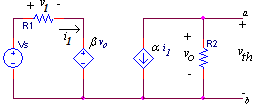
\includegraphics[scale=1]{thevenin}
            \caption{Circuito demonstrativo}\label{thevenin} 
        \end{figure}

    \subsection{Determinação de $v_{th}$}
    
      A tensão do circuito equivalente de Thévenin, $v_{th}$, é a tensão no par de terminais(abertos) escolhidos para a representação do circuito equivalente. Para sua obtenção, os terminais do circuito original que se deseja determinar o circuito equivalente devem ser abertos e, caso estes terminais pertençam a algum elemento, este é retirado do circuito. A tensão em questão pode ser obtida com qualquer método de análise de circuito até aqui apresentada.

\begin{example}

No circuito utilizado para demonstração, na figura \ref{thevenin}, os terminais já se encontram abertos e a tensão $v_{th}$ é dada por:

\begin{equation}\label{vth}
v_{th} = v_o = -R_2 \alpha i_1
\end{equation}

A tensão no resistor $R_2$ é determinada pela corrente gerada pela fonte de corrente dependente $\alpha i_1$ e esta corrente circula pelo resistor de modo que a tensão gerada possui polaridade contrária a polaridade de referência indicada e, por isso, na equação de $v_o$, indicada na equação \ref{vth}, acrescenta-se o sinal $(-)$ para representar essa polaridade invertida.

Da parte do circuito onde está a fonte de tensão independente, escrevendo a equação de tensão para a malha simples formada pelas fontes de tensão e pelo resistor $R_1$, percorrendo a malha no sentido indicado pela corrente $i_1$ e considerando queda de tensão $(+)$, temos:

\begin{equation}
-v_s+v_1+\beta v_o=0
\end{equation}

\begin{equation}
v_1=v_s-\beta v_o \Rightarrow R_1 i_1=v_s-\beta v_o
\end{equation}

Isolando a corrente $i_1$, temos:

\begin{equation}\label{i1}
i_1=\frac{v_s-\beta v_o}{R_1} = \frac{v_s-\beta v_{th}}{R_1}
\end{equation}

Substituindo \ref{i1} em \ref{vth}:

\begin{equation}
v_{th}=v_o=-R_2\alpha\frac{v_s-\beta v_{th}}{R_1}=-\frac{R_2\alpha v_s}{R_1}+\frac{R_2 \alpha\beta v_{th}}{R_1}
\end{equation}

Isolando os termos de $v_{th}$:

\begin{equation}
v_{th}\frac{1-R_2 \alpha\beta}{R_1} =-\frac{R_2\alpha v_s}{R_1} 
\end{equation}

\begin{equation}
v_{th}(R_1-R_2 \alpha\beta)=-R_2\alpha v_s
\end{equation}

\begin{equation}
v_{th}=-\frac{R_2\alpha v_s}{R_1-R_2\alpha\beta}
\end{equation}

\end{example}

    \subsection{Determinação de $R_{th}$}

A resistência do circuito equivalente de Thévenin, que é a mesma para o equivalente de Norton, é definida como a relação entre a tensão de circuito aberto, $v_{th}$ e a corrente de curto-circuito entre esses terminais, $i_n$.

\begin{equation}\label{rth}
R_n = R_{th} = \frac{v_{th}}{i_n}
\end{equation}

Esta resistência também representa a resistência "vista" dos terminais a serem analisados.

\begin{remark}
Na determinação de $R_{th}$, todas as fontes de alimentação \textbf{independentes} precisam ser substituídas pela sua resistência interna. Como as fontes de tensão tem resistência interna nula, na determinação da resistência de Thévenin, devem ser substituídas por curtos-circuitos. Fontes de corrente tem resistência interna infinita e, por isso, devem ser substituídas por circuitos abertos.
\end{remark}

\begin{remark}
Fontes de alimentação \textbf{dependentes} permanecem no circuito no momento da determinação de $R_{th}$.
\end{remark}

        \subsubsection{Método I}{
        
\begin{remark}
O método I só pode ser utilizado quando o circuito contém \textbf{apenas} fontes de alimentação \textbf{independentes}.
\end{remark}        

        \begin{figure}[!htbp] \centering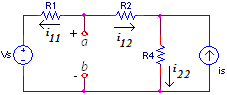
\includegraphics[scale=1]{metodo1}
            \caption{Circuito demonstrativo}\label{metodo1} 
        \end{figure}
        \begin{figure}[!htbp] \centering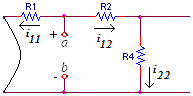
\includegraphics[scale=1]{metodo1aberto}
            \caption{Circuito demonstrativo}\label{metodo1aberto} 
        \end{figure}
        
Devido às restrições do método, o circuito utilizado para exemplificar a utilização será o da figura \ref{metodo1}.

Substituindo as fontes dependentes por suas resistências internas, o circuito a ser analisado está representado na figura \ref{metodo1aberto}.

Observando a partir dos terminais "a" e "b" do circuito, percebe-se que os resistores $R_2$ e $R_4$ estão em série e esta associação está em paralelo com o resistor $R_1$. Sendo assim, a resistência equivalente Thévenin é dada por 

\begin{equation}
R_{th}=\frac{R_1 (R_2+R_4)}{R_1+R_2+R_4}
\end{equation}
}
        
        
        \subsubsection{Método II}{
        
\begin{remark}
O método II só pode ser utilizado quando o circuito contém  fontes de alimentação dependentes e pelo menos uma independente.
\end{remark}

Nesse método, a resistência equivalente Thévenin é determinada a partir da equação \ref{rth}, onde, como já definido anteriormente, $i_{cc}$ é a corrente que passa pelo curto estabelecido entre os terminais "a" e "b", no circuito original, e que corresponde a própria corrente de Norton.

        \begin{figure}[!htbp] \centering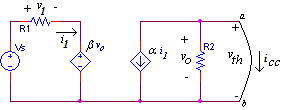
\includegraphics[scale=1]{metodo2aberto}
            \caption{Circuito demonstrativo}\label{metodo2aberto} 
        \end{figure}

Curto circuitando os terminais "a" e "b", conforme mostrado na figura \ref{metodo2aberto}, a tensão vo se anula, já que toda a corrente gerada pela fonte dependente passará pelo curto-circuito. Esse fato também define que $i_{cc}=-\alpha i_1$. O sinal negativo representa o fato de que a corrente de referência $i_{cc}$ circula pelo curto em sentido contrário a corrente real imposta pela fonte de corrente dependente.

Da parte do circuito onde está a fonte de tensão independente, escrevendo a equação de tensão para a malha simples formada pelas fontes de tensão e pelo resistor $R_1$, percorrendo a malha no sentido indicado pela corrente $i_1$ e considerando queda de tensão $(+)$, temos:

\begin{equation}
-v_s+v_1+\beta v_o=0
\end{equation}

\begin{equation}
v_1=v_s-\beta v_o \Rightarrow R_1 i_1=v_s-\beta v_o
\end{equation}

Isolando a corrente $i_1$, e observando que $v_o=0$, temos:

\begin{equation}
i_1=\frac{v_s-\beta v_o}{R_1} = \frac{v_s}{R_1} 
\end{equation}

Substituindo na expressão de $i_{cc}$:

\begin{equation}
i_{cc}=-\alpha\frac{v_s}{R_1}=-\frac{\alpha v_s}{R_1} 
\end{equation}

\begin{equation}
R_{th}=\frac{v_{th}}{i_{cc}} =\frac{\frac{R_2\alpha v_s}{R_1-R_2\alpha\beta}}{-\frac{\alpha v_s}{R_1}} = \frac{R_1 R_2}{R_1-R_2 \alpha\beta}
\end{equation}
}



        \subsubsection{Método III}{        

\begin{remark}
O método III não apresenta restrições em relação às fontes de alimentação.
\end{remark}   

        \begin{figure}[!htbp] \centering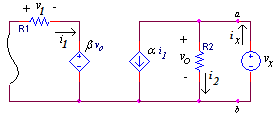
\includegraphics[scale=1]{metodo3}
            \caption{Circuito demonstrativo}\label{metodo3} 
        \end{figure}
   
Nesse método, a resistência equivalente Thévenin é determinada a partir da equação $R_{th}=\frac{v_x}{i_x}$, onde, $v_x$ e $i_x$ são, respectivamente, a tensão e a corrente de uma fonte independente de corrente ou tensão acoplada aos terminais "a" e "b" do circuito original como está indicado na imagem \ref{metodo3}. 

O objetivo quando utiliza-se o método 3 é determinar uma expressão para $v_x$ que seja função de $i_x$, ou vice-versa. Além disso, as expressões devem ser da forma $v_x=f(termos conhecidos do circuito)i_x$, ou $i_x=f(termos conhecidos do circuito)v_x$, dessa forma, quando for calculada a razão $\frac{v_x}{i_x}$, que determina $R_{th}$, constarão apenas os termos conhecidos do circuito.

A partir da LKC podemos escrever a seguinte equação para as correntes é $\alpha i_1$, é $i_2$ e $i_x$.

\begin{equation}
i_x=i_2+\alpha i_1
\end{equation}

Substituindo $i_2$ pela sua expressão em termos de $v_x$, temos:

\begin{equation}\label{ix}
i_x=\frac{v_x}{R_2} +\alpha i_1
\end{equation}

Da parte do circuito onde está a fonte de tensão dependente, escrevendo a equação de tensão para a malha simples formada pela fonte de tensão e pelo resistor $R_1$, percorrendo a malha no sentido indicado pela corrente $i_1$ e considerando queda de tensão (+), temos:

\begin{equation}
v_1+\beta v_o=0
\end{equation}

\begin{equation}
v_1=-\beta v_o \Rightarrow R_1 i_1=-\beta v_o
\end{equation}

Isolando a corrente $i_1$ e observando que $v_o=v_x$, temos:

\begin{equation}\label{i1}
i_1=-\frac{\beta v_o}{R_1} =-\frac{\beta v_x}{R_1} 
\end{equation}

Substituindo \ref{i1} em  \ref{ix}:

\begin{equation}
i_x=\frac{v_x}{R_2} -\alpha\frac{\beta v_x}{R_1} = v_x\frac{R_1-\alpha\beta R_2}{R_1 R_2}
\end{equation}

\begin{equation}
R_{th} = \frac{v_x}{i_x} = \frac{v_x}{v_x\frac{R_1-\alpha\beta R_2}{R_1 R_2}} = \frac{R_1 R_2}{R_1-R_2 \alpha\beta}
\end{equation}
}

\begin{remark}
Quando o circuito apresenta fontes dependentes, existe a possibilidade de se obter valores de resistência equivalente Thévenin \textbf{NEGATIVAS}. Uma resistência negativa indica um elemento fornecedor de energia. Esse comportamento está, de fato, refletindo um comportamento conjunto de todas as fontes e outros elementos do circuito original e não pode ser vista estritamente como uma resistência pura. No caso de circuitos contendo apenas fontes independentes de fato a resistência equivalente Thévenin representa efetivamente uma resistência. 
\end{remark}
   
    \subsection{Máxima transferência de potência}{

O estudo da máxima transferência de potência permite identificar se um dado componente, que consome energia, está recebendo do circuito ao qual está acoplado o máximo de potência que aquele pode transferir.

A condição para que haja a máxima transferência de potência é que a resistência de um dado elemento consumidor seja igual a resistência equivalente Thévenin, vista dos terminais do referido elemento, como será demonstrado a seguir.

\begin{figure}[!htbp] \centering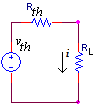
\includegraphics[scale=1]{thmax}
            \caption{}\label{thmax} 
        \end{figure}

Considerando o circuito na figura \ref{thmax} é possível observar que a representação do circuito equivalente Thévenin, visto dos terminais de um resistor $R_L$. Para verificar a afirmação de que se $R_L=R_{th}$, temos a máxima transferência de potência, deve-se determinar a expressão de potência no resistor $R_L$, que é dada por:

\begin{equation}\label{pth}
P_{R_L} = R_L i^2 = R_L \frac{v_{th}}{R_L+R_{th}} = \frac{R_L v_{th}^2}{(R_L+R_th)^2} 
\end{equation} 

Derivando a expressão \ref{pth} e igualando a zero, determina-se o ponto de máximo ou mínimo da mesma. A derivada será realizada em relação à $R_L$, visto que é o termo que pode ser alterado para satisfazer a condição de máxima transferência de potência.

\begin{equation}
\frac{dP_{R_L}}{dR_L}= \frac{v_{th}^2}{(R_L+R_{th})^2} -2\frac{R_L v_{th}^2}{(R_L+R_{th})^3} =0
\end{equation}

\begin{equation}
\frac{v_{th}^2}{(R_L+R_{th})^2} = 2\frac{R_L v_{th}^2}{(R_L+R_{th})^3}
\end{equation}

\begin{equation}
1=\frac{2R_L}{R_L+R_{th}} \Rightarrow R_L+R_{th}=2R_L \Rightarrow R_L=R_{th}
\end{equation}

O cálculo da derivada segunda demonstrará que quando $R_L=R_{th}$, a expressão de $P_{R_L}$ apresenta um ponto de máximo.

O valor da potência máxima transferida para $R_L$, quando o mesmo é igual a $R_{th}$, é determinado pela expressão:

\begin{equation}
P_{R_{L_{máx}}}=\frac{R_{th} v_{th}^2}{(R_{th}+R_{th})^2} =\frac{v_{th}^2}{4R_{th}}
\end{equation}

\begin{figure}[!htbp] \centering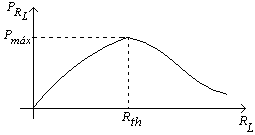
\includegraphics[scale=1]{pxr}
            \caption{}\label{pxr} 
        \end{figure}

Na figura \ref{pxr} é apresentado o gráfico do comportamento da curva de $P_{R_L}$ em função da resistência $R_L$.

\begin{remark}

A potência máxima transferida para uma carga sempre será menor ou igual a metade da potência total gerada no circuito que alimenta a carga.

\end{remark}

\begin{remark}

Para determinar se um dado elemento consumidor em um circuito recebe a máxima potência que o circuito poderia fornecer, basta determinar a resistência equivalente Thévenin, $R_{th}$, do circuito, vista dos terminais do respectivo elemento. Se, e somente se,  $R_{th}$ for igual a resistência do elemento, então estará havendo máxima transferência de potência.

\end{remark}

    }
    
\section{Método da superposição}{

O método de superposição de análise de circuitos aplica-se a circuitos lineares invariantes no tempo. Neste método, a obtenção das grandezas de interesse do circuito, correntes e/ou tensões, ocorre por meio da soma de parcelas dessas grandezas, determinadas considerando a operação \textbf{ISOLADA} de cada fonte independente presente no circuito.

        \begin{figure}[!htbp] \centering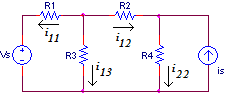
\includegraphics[scale=1]{superposicao}
            \caption{}\label{superposicao} 
        \end{figure}
        
        \begin{figure}[!htbp] \centering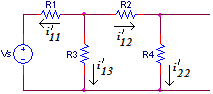
\includegraphics[scale=1]{superposicaoVs}
            \caption{Contribuição de $v_s$}\label{superposicaoVs} 
        \end{figure}
        
        \begin{figure}[!htbp] \centering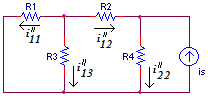
\includegraphics[scale=1]{superposicaoIs}
            \caption{Contribuição de $i_s$}\label{superposicaoIs} 
        \end{figure}

Para exemplificar a aplicação do método, considere o circuito da figura \ref{superposicao}, onde se deseja determinar as correntes $i_{11}$, $i_{12}$, $i_{13}$ e $i_{22}$. Para isso, serão determinadas parcelas $i_{11}^{'}$, $i_{12}^{'}$, $i_{13}^{'}$ e $i_{22}^{'}$, $i_{11}^{''}$, $i_{12}^{''}$, $i_{13}^{''}$ e $i_{22}^{''}$, onde as parcelas $i_{xy}^{'}$ serão obtidas considerando o circuito operando apenas com a fonte de tensão $v_s$, como no circuito da figura \ref{superposicaoVs}, e as parcelas $i_{xy}^{''}$ serão obtidas considerando o circuito operando apenas com a fonte de corrente $i_s$, como na figura \ref{superposicaoIs}.

como as parcelas $i_{xy}^{'}$ e $i_{xy}^{''}$ mantiveram o mesmo sentido das correntes originalmente definidas no circuito com todas as fontes, o cálculo da componente total é realizado somando-se as parcelas $i_{xy}^{'}$ e $i_{xy}^{''}$, ou seja:

\begin{equation}
\left\{\begin{aligned} & 
        i_{11}=i_{11}^{'}+i_{11}^{''}\\& 
        i_{12}=i_{12}^{'}+i_{12}^{''}\\& 
        i_{13}=i_{13}^{'}+i_{13}^{''}\\&
        i_{22}=i_{22}^{'}+i_{22}^{''}
    \end{aligned}\right.
\end{equation}

Também deve ser observado que a eliminação das fontes de tensão é realizada curto circuitando os terminais das mesmas, enquanto as fontes de corrente devem ter seus terminais abertos.

\begin{remark}
A escolha do sentido das parcelas de corrente e polaridade das parcelas de tensão não precisa obrigatoriamente ser definidas em função dos sentidos e/ou polaridades das grandezas originalmente definidas no circuito com todas as fontes. Embora não seja obrigatório usar para as parcelas os sentidos de corrente e polaridades de tensão das grandezas do circuito original, a adoção dos mesmos proporciona um cálculo das grandezas totais bem simples, bastando apenas somar as parcelas.
\end{remark}

\begin{remark}
Fontes dependentes não são eliminadas na análise.
\end{remark}

}


	 
%----------------------------------------------------------------------------------------
%	PART
%----------------------------------------------------------------------------------------

\part{Segundo Estágio}{

%----------------------------------------------------------------------------------------
%	CHAPTER 7
%----------------------------------------------------------------------------------------
	
\chapterimage{includes/documents/chapter_head_2.pdf} % Chapter heading image
\chapter{Indutância}

\section{Definições}

\begin{definition}[Permeabilidade magnética $(\mu)$] Medida da facilidade com que linhas de campo magnético podem ser estabelecidas no interior de um material. A expressão da permeabilidade é dada por:

\begin{equation}
\mu = \frac{B}{H}
\end{equation}

Onde $B (\frac{Weber}{m^2})$ é a densidade de fluxo magnético e $H (\frac{A}{m})$ é o vetor campo magnético.

\end{definition}

\begin{definition}[Densidade de fluxo magnético $(B)$ ]Número de linhas de campo por unidade de área.

\begin{equation}
B = \frac{\Phi}{A}
\end{equation}

\end{definition}

\begin{definition}[Relutância $\mathfrak{R}$ ]Oposição ao estabelecimento do fluxo magnético. É o análogo da resistência elétrica para circuitos magnéticos.

\begin{equation}
\mathfrak{R} = \frac{l}{\mu_0\mu_rA}
\end{equation}

Onde $l(m)$ é o comprimento do circuito, $A(m^2)$ é a área e $\mu_0\mu_r(\frac{Henry}{m})$ a permeabilidade magnética do material.

\end{definition}

\begin{definition}[Força magnetomotriz $\mathfrak{F}$] A força magnetomotriz é um artifício matemático utilizado para medir a intensidade do campo por meio da corrente elétrica que o gera. A força magnetomotriz é dada por:

\begin{equation}
\mathfrak{F} = Ni = Hl
\end{equation}

Onde $N$ é o número de espiras, $(A)$ a corrente, $H(\frac{A}{m})$ o campo magnético e $l(m)$ o comprimento. 

\end{definition}

\section{Equivalência de Hopkingson e lei de Ohm para circuitos magnéticos}

O equivalente de Hopkingson é uma forma de apresentar um circuito magnético com características semelhantes às dos circuitos elétricos resistivos. A associação consiste em comparar a força magnetomotriz com a força eletromotriz, a relutância magnética com a resistência elétrica e o fluxo magnético com a corrente elétrica. Desta forma, a lei de Ohm para circuitos magnéticos é dada por:

\begin{equation}
\mathfrak{F} = \mathfrak{R}\Phi
\end{equation}


\section{Indutância}

\begin{equation}\label{faraday}
\oint_c \vec{E}\cdot\vec{dl} = -\frac{d\Phi}{dt}
\end{equation}

A lei de Faraday, que é uma das quatro equações de Maxwell e está expressa na equação \ref{faraday}, estabelece uma relação entre a taxa de variação do fluxo magnético e a tensão induzida. A indutância é o parâmetro que relaciona a tensão induzida e a corrente que gera o fluxo magnético. A relação é dada por:

\begin{equation}\label{lambdai}
\lambda(i) = L(i)di
\end{equation}

Se a relação \ref{lambdai} for linear, $L(i)$ é uma constante.

    \subsection{Indutância própria}
\begin{definition}[Indutância própria]
Propriedade de um condutor de gerar uma força eletromotriz (tensão induzida) sobre ele próprio quando submetido a uma corrente elétrica variável. Nessa condição, é gerada uma força eletromotriz no sentido contrário à variação de corrente à qual o indutor está submetido, ou seja, o indutor tende a manter o fluxo de campo magnético inalterado.
\end{definition}

Se for considerado um elemento indutivo composto por uma bobina de "N" espiras envoltas em um núcleo de área "A", tem-se que, quando submetido a uma corrente "i", esta bobina desenvolverá um fluxo magnético dado pela lei de Ohm para campos magnéticos por:

\begin{equation}\label{fluxoM}
 \Phi = \frac{\mathfrak{F}}{\mathfrak{R}} = \frac{Ni}{\mathfrak{R}}
\end{equation}    
    
Como indicado em \ref{fluxoM}, se a corrente circulando pela bobina for variável, será autoinduzida uma tensão na mesma dada por:

\begin{equation}
e = N\frac{d\Phi}{dt}
\end{equation}

Pela regra da cadeia é possível escrever:

\begin{equation}
e = N \frac{d\phi}{di}\frac{di}{dt} = L\frac{di}{dt}
\end{equation}

Por \ref{fluxoM}, é verdade que:

\begin{equation}\label{LNR}
L = N\frac{\frac{Ni}{\mathfrak{R}}}{di} = \frac{N^2}{\mathfrak{R}}
\end{equation}   

\begin{figure}[!htbp] \centering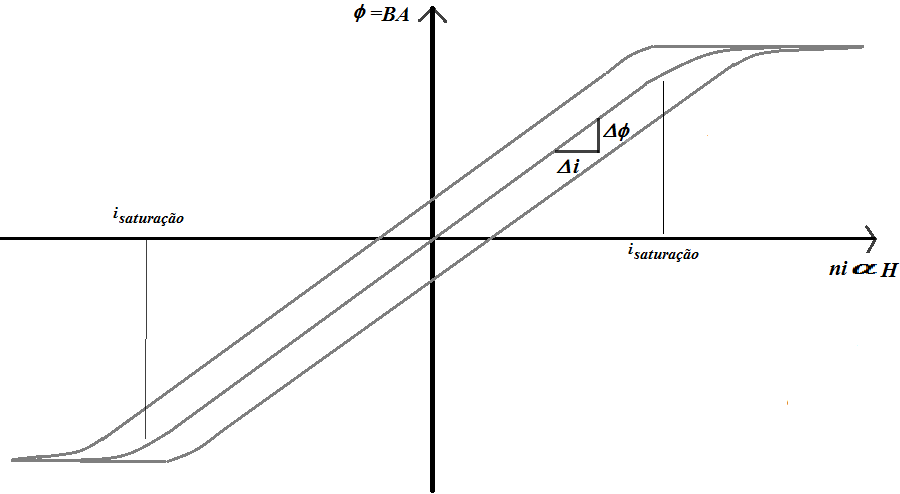
\includegraphics[scale=0.5]{histerese}
            \caption{Curva de histerese}\label{histerese} 
        \end{figure}

Em indutores reais a indutância própria apresenta uma faixa de operação linear, na qual a relação entre fluxo $\Phi$ e a corrente $i$ é linear e a partir de um nível de corrente, $i_{\text{saturação}}$, apresenta um comportamento de saturação, o que justifica a desproporcionalidade da relação. Esse comportamento pode ser visualizado a partir da curva de histerese, que relaciona "B" e "H". Como $B=\frac{\Phi}{A}$ e $H = N\frac{i}{l}$, é possível analisar a curva de histerese em termos do fluxo e da corrente. 

Observando a curva na figura \ref{histerese}, percebe-se que após a corrente de saturação ser atingida, uma mesma variação $\Delta i$ não mais provocará igual variação $\Delta\Phi$. Como a indutância pode ser dada por \ref{LNR}, que pode ser aproximada por $L = \frac{\Delta\Phi}{\Delta i}$, percebe-se que após a saturação, $\Delta\Phi$ tende a zero, logo, a indutância tende a zero na região de saturação.

Em um indutor com indutância própria "L", a polaridade da tensão reflete a reação do campo magnético à corrente responsável pela sua existência.

\begin{remark}
Quando $i$ aumenta, $\frac{di}{dt} > 0 \Rightarrow v_L > 0$. Nessa condição é preciso fornecer energia ao indutor para criação ou aumento do campo magnético.
\end{remark}

\begin{remark}
Quando $i$ diminui, $\frac{di}{dt} < 0 \Rightarrow v_L < 0$. Nessa condição o indutor devolve energia para o circuito, retirando-a do campo magnético.
\end{remark}

\begin{remark}
A polaridade de referência adotada é aquela em que o potencial é positivo no terminal do indutor onde a corrente circulando pelo mesmo entra
\end{remark}


\begin{remark}
Pela convenção passiva, a tensão auto-induzida é uma queda de tensão no sentido da corrente que a gera.
\end{remark}


\begin{remark}
Todo indutor real é especificado pela sua indutância e pela sua corrente de trabalho. Essa corrente indica o maior nível de corrente que o indutor suporta sem que o mesmo entre na região de saturação.
\end{remark}
    
    \subsection{Indutância mútua}
    
    \begin{definition}
Propriedade de um condutor de gerar uma força eletromotriz (tensão induzida) sobre um outro condutor quando submetido a uma corrente elétrica variável.
    \end{definition}
    
\begin{figure}[!htbp] \centering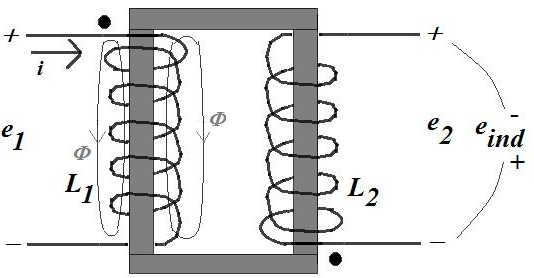
\includegraphics[scale=0.5]{indutanciaM}
            \caption{Curva de histerese}\label{indutanciaM} 
        \end{figure}    
    
    Na figura \ref{indutanciaM}, o circuito contém duas bobinas acopladas magneticamente através de um núcleo de material com permeabilidade maior que a do ar, que faz com que a quase totalidade das linhas de campo magnético geradas pela corrente $i$, que circula pela bobina de indutância $L$, fiquem confinadas no material do núcleo. Como as espiras da bobina de indutância $L_2$ concatenam estas linhas de campo, se houver uma variação de direção e/ou amplitude dessas linhas de campo magnético, será induzida uma tensão nos terminais da bobina de indutância $L_2$. A determinação da polaridade da tensão induzida, em relação a tensão de referência $e_2$, dependerá da polaridade de acoplamento das bobinas, que é indicada pelos pontos observados na figura.

\section{Indutor}
\begin{figure}[!htbp] \centering
                \begin{circuitikz}[scale=3]
	                \draw (0,0) to [cute inductor=$L$, v=$v_L$, i=$i_L$] (2,0);
	            \end{circuitikz}
        \caption{Símbolo segundo a norma americana}\label{indutor} 
        \end{figure} 
        
        \begin{figure}[!htbp] \centering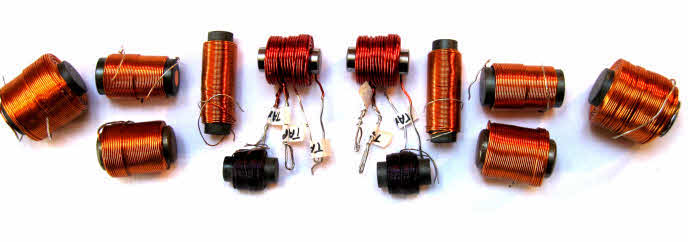
\includegraphics[scale=0.5]{indutores}
            \caption{Aspecto físico}\label{aspectoL} 
        \end{figure}
 
O indutor é o componente eletrônico com capacidade de armazenar energia em um campo magnético. É responsável por provocar defasamento entre a tensão e a corrente, de forma que a corrente é atrasada em relação à tensão. Na figura \ref{indutor} é apresentado o símbolo associado aos indutores e na imagem \ref{aspectoL} é possível observar o aspecto físico de alguns indutores.

Uma aplicação prática dos indutores está nos sensores de presença indutivos. Quando algum objeto com massa metálica entra nas linhas de campo de um indutor, as linhas de campo tendem a abandonar o ar e a passar por dentro do objeto. Isso implica numa modificação no valor das grandezas elétricas no indutor devido às propriedades físicas da indutância. Os sensores eletrônicos de proximidade são utilizados largamente em todos os lugares onde as condições de trabalho são extremas, tais como: óleos lubrificantes, óleos solúveis, óleos de corte, vibrações, onde são exigidos altos níveis de vedação e robustez.

\begin{equation}
\left\{\begin{aligned} & 
        v_L=L\frac{di_l}{dt}\\& 
        i_l=\frac{1}{L}\int v_L(t)dt + i_L(0)\\& 
        \omega_L=\frac{1}{2}Li_L^2
    \end{aligned}\right.
\end{equation}

Das expressões do indutor, podem ser observadas algumas características de funcionamento que são importantes para o dispositivo:

\begin{remark}
Sob condição de corrente constante, ou seja, $\frac{di}{dt}=0$, o indutor comporta-se como um curto-circuito.
\end{remark}

\begin{remark}
	A corrente que atravessa um indutor não pode variar na forma de um degrau, ou seja, não pode apresentar uma descontinuidade, isso implicaria em um $\frac{di}{dt}\rightarrow\infty$. Dessa forma, conclui-se que o indutor é um dispositivo amortecedor de oscilações de corrente.
\end{remark}

\begin{remark}
Quando submetido a um impulso de tensão, a corrente de um indutor pode apresentar uma mudança na forma de um degrau, porém, um impulso de tensão apresenta energia infinita.
\end{remark}

\section{Determinação da polaridade de acoplamento}

    \subsection{Forma de bobinamento conhecida}
    
        \begin{figure}[!htbp] \centering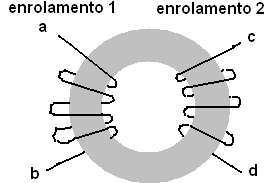
\includegraphics[scale=0.5]{acoplamento}
            \caption{Acoplamento}\label{acoplamento} 
        \end{figure}    
    
    Considerando os enrolamento 1 e 2 acoplados, que compartilham o mesmo núcleo toroidal, como indicado na figura \ref{acoplamento}. Para determinar a polaridade de acoplamento entre os indutores seguimos o procedimento descrito a seguir:
    
    \begin{enumerate}
    \item Escolhe-se arbitrariamente um terminal de um dos enrolamentos e a ele associa um ponto de referência.
    \item Define-se uma corrente entrando neste terminal e a partir da regra da mão direita determina-se o sentido do fluxo gerado por esta corrente.
    \item Escolhe-se arbitrariamente um dos terminais do segundo enrolamento e define-se um sentido de corrente, arbitrário, para este terminal.
    \item Utiliza-se a regra da mão direita para determinar o sentido do fluxo gerado pela curva.
    \item Comparam-se os sentidos dos fluxos identificados nos passos 2 e 4 e estabelece-se o ponto no segundo enrolamento da seguinte forma:
    \begin{itemize}
    \item Fluxos no mesmo sentido: Assinala-se com um ponto o terminal do segundo enrolamento onde a corrente está entrando.
    \item Fluxos em sentido contrário: Assinala-se com um ponto o terminal do segundo enrolamento onde a corrente está saindo.
    \end{itemize}     
    \end{enumerate}
       
    
    \subsection{Forma de bobinamento desconhecida}
    
        \begin{figure}[!htbp] \centering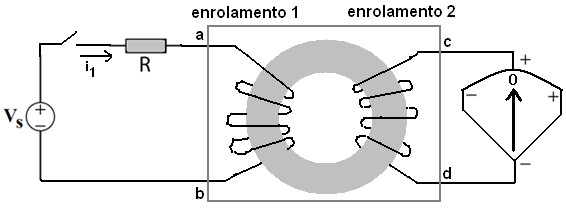
\includegraphics[scale=0.5]{acoplamentoDesconhecido}
            \caption{Acoplamento}\label{acoplamentoDesconhecido} 
        \end{figure}     
    
    Considere os enrolamento 1 e 2 acoplados, que compartilham o mesmo núcleo magnético, como indicado na figura \ref{acoplamentoDesconhecido}. No entanto, diferentemente do caso anterior, não se tem informação da forma como os mesmos são bobinados. Neste caso, para determinar a polaridade de acoplamento entre os indutores, recomendam-se os procedimentos descritos a seguir:
    
    \begin{enumerate}
    \item Conecta-se a um dos enrolamentos uma fonte de tensão CC, chave liga/desliga e resistor. Ao outro enrolamento conecta-se um voltímetro CC, que pode indicar tensões positivas e negativas. No terminal do enrolamento onde será aplicada a tensão positiva da fonte é atribuído o ponto de referência.
    \item Após a conexão a chave liga desliga é acionada. Em uma sequência rápida a mesma é ligada e desligada, de modo que um pulso de tensão é aplicado ao enrolamento 1. Com a aplicação do pulso de tensão uma corrente entra no terminal em que foi conectado o potencial positivo da fonte.
    \item No enrolamento onde está conectado o voltímetro CC observa-se o sinal da tensão que foi gerada e a partir desse atribui-se o ponto a um dos terminais do enrolamento 2 seguindo a seguinte regra:
    \begin{itemize}
    \item Se a tensão gerada for positiva, o ponto é atribuído ao terminal do enrolamento 2 conectado ao terminal positivo (+) do voltímetro CC.
    \item	Se a tensão gerada for negativa, o ponto é atribuído ao terminal do enrolamento 2 conectado ao terminal negativo (-) do voltímetro CC.
    \end{itemize}
    \end{enumerate}
    
    \subsection{Regra do ponto}

\begin{remark}
Quando o sentido de referência da corrente em um ramo contendo um indutor acoplado entra no terminal ponto deste, esta corrente induzirá uma tensão cujo potencial positivo (+) será atribuído ao terminal ponto do respectivo indutor acoplado.
\end{remark}


\section{Associação de indutores}

    \subsection{Indutores não acoplados}
    
        \subsubsection{Ligação em série}

 \begin{figure}[!htbp] \centering
 \begin{circuitikz}
     \draw
         (0,2)to[cute inductor =$L_1$,v=$v_1$](2,2)
              to[cute inductor =$L_2$,v=$v_2$](4,2)
              to                              (5,2)
              to[cute inductor =$L_3$,v=$v_3$](5,0)
              to                              (4,0)
              to[cute inductor =$L_4$,v=$v_4$](2,0)
              to[cute inductor =$L_5$,v=$v_5$](0,0)
         (-0.05,2) to[open, v=$v$](-0.05,0)
     ;
 \end{circuitikz}
            \caption{Indutores em série}\label{indutorSerie} 
        \end{figure}
        
        \begin{figure}[!htbp] \centering
 \begin{circuitikz}
     \draw
         (0,2)to                              (1,2)
              to[cute inductor =$L_{eq}$](1,0)
              to                              (0,0)
              
         (-0.05,2) to[open, v=$v$](-0.05,0)
     ;
 \end{circuitikz}
            \caption{Indutor equivalente}\label{indutorEquivlente} 
        \end{figure}

Considerando o circuito formado por um conjunto de indutores, todos conectados em série, como o apresentado na figura \ref{indutorSerie}. A associação dos indutores pode ser substituída por um único indutor, cujo valor é determinado na sequência.

Usando a LKT, temos:

\begin{equation}
v = v_1+v_2+v_3+v_4+v_5
\end{equation}  

\begin{equation}
v = L_1\frac{di}{dt} +L_2\frac{di}{dt} +L_3\frac{di}{dt} +L_4\frac{di}{dt} +L_5\frac{di}{dt}
\end{equation}  

Com $\frac{di}{dt}$ em evidência:

\begin{equation}
v = (L_1+L_2+L_3+L_4+L_5)\frac{di}{dt}
\end{equation}

Observando o circuito equivalente pretendido, que contém uma indutância equivalente $L_{eq}$, a expressão de tensão é dada por:

\begin{equation}
v=L_{eq}\frac{di}{dt}
\end{equation}

Logo:

\begin{equation}
L_{eq}=L_1+L_2+L_3+L_4+L_5
\end{equation}

De modo geral:

\begin{equation}
L_{eq} = \sum\limits_{\alpha = 1}^{n} L_\alpha
\end{equation}        
        
        \subsubsection{Ligação em paralelo}
    
\begin{figure}[!htbp] \centering
 \begin{circuitikz}
     \draw
         (0,0) to (2,0) to (4,0) to (6,0) to (8,0) to(10,0)
         (0,2) to[short, i=$i$] (2,2) to (4,2) to (6,2) to (8,2) to(10,2)
         (0,2) to[open, v=$v$] (0,0)
         (2,0) to[cute inductor =$L_1$, i<=$i_{L_1}$](2,2)
         (4,0) to[cute inductor =$L_2$, i<=$i_{L_2}$](4,2)
         (6,0) to[cute inductor =$L_3$, i<=$i_{L_3}$](6,2)
         (8,0) to[cute inductor =$L_4$, i<=$i_{L_4}$](8,2)
         (10,0)to[cute inductor =$L_5$, i<=$i_{L_5}$](10,2)
     ;
 \end{circuitikz}
            \caption{Indutores em paralelo}\label{indutorParalelo} 
        \end{figure}    
    
Considerando o circuito formado por um conjunto de indutores, todos conectados em paralelo, como o apresentado na figura \ref{indutorParalelo}. A associação dos indutores pode ser substituída por um único indutor, cujo valor é determinado na sequência.

Pela LKC:

\begin{equation}
i = i_{L_1}+i_{L_2}+i_{L_3}+i_{L_4}+i_{L_5}
\end{equation}

\begin{equation}
i =  \frac{1}{L_1}\int v(t)dt + \frac{1}{L_2}\int v(t)dt + \frac{1}{L_3}\int v(t)dt + \frac{1}{L_4}\int v(t)dt + \frac{1}{L_5}\int v(t)dt 
\end{equation}

\begin{equation}
i = (\frac{1}{L_1}+\frac{1}{L_2}+\frac{1}{L_3}+\frac{1}{L_4}+\frac{1}{L_5})\int v(t)dt
\end{equation}

Observando o circuito equivalente pretendido, que contém uma indutância equivalente $L_{eq}$, a expressão de corrente é dada por:

\begin{equation}
i = \frac{1}{L_{eq}}\int v(t)dt
\end{equation}

\begin{equation}
\frac{1}{L_{eq}} = \frac{1}{L_1}+\frac{1}{L_2}+\frac{1}{L_3}+\frac{1}{L_4}+\frac{1}{L_5}
\end{equation}

De modo geral:

\begin{equation}
\frac{1}{L_{eq}} = \sum\limits_{\alpha = 1}^{n}\frac{1}{L_\alpha}
\end{equation}
    
    \subsection{Indutores acoplados}
        \subsubsection{Ligação em série}
        %TODO Circuito em série acoplado
\begin{figure}[!htbp] \centering
 \begin{circuitikz}
     \draw
     
         (0.75,2.25)node{$\bullet$}
         (3.25,1.75)node{$\bullet$}
         (0,3)node{}
         (0,2)to[cute inductor =$L_1$,v=$v_1$](3,2)
              to[cute inductor =$L_2$,v=$v_2$](3,0)
              to                              (0,0)
              
         (0,2) to[open, v=$v$](0,0)
     ;
 \end{circuitikz}
            \caption{Indutores em série acoplados magneticamente}\label{indutorSerieAcoplado} 
        \end{figure}         
        
Considere o segmento de circuito formado por dois indutores conectados em série e magneticamente acoplados, como apresentado na figura \ref{indutorSerieAcoplado}. A associação desses indutores pode ser substituída por um único indutor, cujo valor é determinado na sequência.

Usando a LKT e considerando queda de tensão positiva:

\begin{equation}
v=v_1+v_2
\end{equation}
  
\begin{equation}
v=L_1\frac{di}{dt}+M_{12}\frac{di}{dt}+L_2\frac{di}{dt}+M_{12}\frac{di}{dt}
\end{equation} 

Observando que aparecem dois termos de tensão induzida, um para cada indutor, os quais são determinados por meio do produto entre a indutância mútua, representada por $M_{12}$ e a derivada da corrente que circula pelo indutor que induzirá tensão no outro. Para a determinação do sinal das tensões induzidas, foi utilizada a regra do ponto. No exemplo da figura \ref{indutorSerieAcoplado}, percebe-se que as correntes entram nos terminais ponto de ambos os indutores, logo, as tensões induzidas por cada um dos mesmos terão sinais positivos nos respectivos terminais ponto dos indutores. Pela convenção adotada, quando percorre-se a malha no sentido da corrente, tanto para a tensão devida a indutância própria, como para o termo de tensão induzida, percebe-se que há uma queda de tensão, logo, os sinais de tensão, própria e induzida, serão positivos na equação. Com $\frac{di}{dt}$ em evidência:

\begin{equation}
v=\frac{di}{dt}(L_1+L_2+2M_{12})
\end{equation}

Observando o circuito equivalente pretendido, que contém uma indutância equivalente $L_{eq}$, a expressão de tensão é dada por:

\begin{equation}
v=L_{eq}\frac{di}{dt}
\end{equation}

\begin{equation}
L_{eq}=L_1+L_2+2M_{12}
\end{equation}
    
        
        \subsubsection{Ligação em paralelo}
        
%TODO Circuito em paralelo acoplado
\begin{figure}[!htbp] \centering
 \begin{circuitikz}
     \draw
         (1.5,0.5)node{$\bullet$}
         (3.5,0.5)node{$\bullet$}
         (0,0) to (2,0) to (4,0) 
         (0,2) to[short, i=$i$] (2,2) to (4,2)
         (0,2) to[open, v=$v$] (0,0)
         (2,0) to[cute inductor =$L_1$, i<=$i_{L_1}$](2,2)
         (4,0) to[cute inductor =$L_2$, i<=$i_{L_2}$](4,2)
         
         
         
     ;
 \end{circuitikz}
            \caption{Indutores em paralelo acoplados magneticamente}\label{indutorParaleloAcoplado} 
        \end{figure}         
        
 Considerando o segmento de circuito formado por dois indutores conectados em paralelo e magneticamente acoplados, como apresentado na figura \ref{indutorParaleloAcoplado}. A associação desses indutores pode ser substituída por um único indutor, cujo valor é determinado na sequência.
 
 Usando a LKC:
 
 \begin{equation}
 i=i_1+i_2
 \end{equation}
 
 Escrevendo as expressões de fluxo:
 
\begin{equation}
\left\{\begin{aligned} & 
        \Phi_1=L_1 i_1+M_{12} i_2\\& 
        \Phi_2=M_{12} i_1+L_2 i_2
    \end{aligned}\right.
\end{equation}

As componentes de fluxo devidas as indutâncias mútuas são positivas, isso ocorre porque as correntes circulando em cada enrolamento reforçam o fluxo mutuamente.

Escrevendo as expressões na forma matricial, temos:
\begin{equation}
\begin{bmatrix}
\Phi_1\\\Phi_2
\end{bmatrix}
=
\begin{bmatrix}
L_1 & M_{12} \\
M_{12} & L_2 
\end{bmatrix}
\begin{bmatrix}
 i_1\\i_2
\end{bmatrix}
\end{equation}

A matriz $\begin{bmatrix}L_1 & M_{12} \\M_{12} & L_2\end{bmatrix}$. Resolvendo a equação matricial, é possível determinar os valores das correntes.

\begin{equation}
\begin{bmatrix}
i_1\\i_2
\end{bmatrix}
=
\begin{bmatrix}
\Gamma_1 & \Gamma_{12}\\
\Gamma_{12} & \Gamma_2
\end{bmatrix}
\begin{bmatrix}
\Phi_1\\\Phi_2
\end{bmatrix}
\end{equation}

\begin{equation}
\Gamma_1 = \frac{L_2}{det\begin{bmatrix}
L_1 & M_{12} \\M_{12} & L_2
\end{bmatrix}}
\end{equation}

\begin{equation}
\Gamma_2 = \frac{L_1}{det\begin{bmatrix}
L_1 & M_{12} \\M_{12} & L_2
\end{bmatrix}}
\end{equation}

\begin{equation}
\Gamma_{12} = -\frac{M_{12}}{det\begin{bmatrix}
L_1 & M_{12} \\M_{12} & L_2
\end{bmatrix}}
\end{equation}

Da conexão paralela, $v(t)=v_1(t)=v_2(t)$. Se $i_1(0)=0$ e $i_2(0)=0$, então $\Phi_1(0)=L_1 0+M_12 0= 0$ e $\Phi_2 (0)=M_12+L_2 0=0$. Dado que $v_1 (t)=\frac{d\Phi_1}{dt}$ e $v_2(t)=\frac{d\Phi_2}{dt}$, conclui-se que $\Phi_1(t)=\Phi_2(t)=\Phi(t)$. 
Escrevendo a equação de corrente dada pela LKC:

\begin{equation}\label{eqFlux1}
i=i_1+i_2=\Gamma_1 \Phi_1+\Gamma_{12} \Phi_2+\Gamma_12 \Phi_1+\Gamma_2 \Phi_2=\Phi(\Gamma_1+\Gamma_2+2\Gamma_{12} )
\end{equation}

Considerando o circuito equivalente e escrevendo a expressão do fluxo para o mesmo:

\begin{equation}\label{eqFlux2}
\Phi=L_{eq} i \Rightarrow i=\frac{1}{L_{eq}}\Phi
\end{equation}

Comparando \ref{eqFlux1} e \ref{eqFlux2}:

\begin{equation}
 \frac{1}{L_{eq}} = \Gamma_1+\Gamma_2+2\Gamma_{12}
\end{equation}



            
%----------------------------------------------------------------------------------------
%	CHAPTER 8
%----------------------------------------------------------------------------------------
	
\chapterimage{includes/documents/chapter_head_2.pdf} % Chapter heading image
\chapter{Capacitância}  

\section{Definições}

\begin{definition}[Capacitância]
Grandeza que relaciona a quantidade de cargas por volt armazenada em condutores carregados e separados por meios dielétricos.

\begin{equation}
C = \frac{Q}{V}
\end{equation}

Onde $C (Farad)$ é a capacitância, $Q (Coulumb)$ e $V (Volt)$ a tensão entre os condutores. 

\end{definition}

\begin{definition}[Material dielétrico] É a classe de materiais que, a princípio, não permitem a passagem de corrente elétrica, mas podem ser polarizados e conduzir uma corrente enquanto a polarização não está completa.
\end{definition}

\begin{definition}[Permissividade]
Facilidade com que o dielétrico permite o estabelecimento de linhas de campo no seu interior. Quanto maior a permissividade de um dielétrico, maior a quantidade de carga depositada nas placas por unidade de área das mesmas.
\end{definition}

\begin{definition}[Rigidez dielétrica]É a tensão máxima por unidade de comprimento do dielétrico que o material suporta sem que haja a ruptura e condução de corrente elétrica.
\end{definition}

\section{Capacitor}

\begin{figure}[!htbp] \centering
                \begin{circuitikz}[scale=3]
	                \draw (0,0) to [C=$C$, v=$v_C$, i=$i_C$] (2,0);
	            \end{circuitikz}
        \caption{Símbolo segundo a norma americana}\label{capacitor} 
        \end{figure} 
        
        \begin{figure}[!htbp] \centering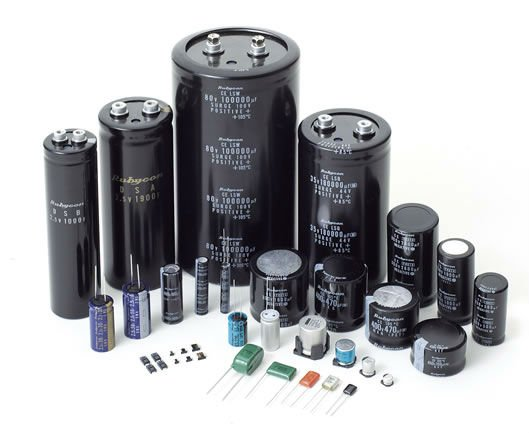
\includegraphics[scale=0.5]{aspectoC}
            \caption{Aspecto físico}\label{aspectoC} 
        \end{figure}
 
O capacitor é o componente eletrônico com capacidade de armazenar energia em um campo elétrico. É responsável por provocar defasamento entre a tensão e a corrente, de forma que a corrente é adiantada em relação à tensão. Na figura \ref{capacitor} é apresentado o símbolo associado aos indutores e na imagem \ref{aspectoC} é possível observar o aspecto físico de alguns capacitores.

\begin{equation}
\left\{\begin{aligned} & 
        i_c=C\frac{dv_c}{dt}\\& 
        v_c=\frac{1}{C}\int i_c(t)dt + i_c(0)\\& 
        \omega_c=\frac{1}{2}Cv_c^2
    \end{aligned}\right.
\end{equation}

    \subsection{Associação em série}
 \begin{figure}[!htbp] \centering
 \begin{circuitikz}
     \draw
         (0,2) to[C=$C_1$, v=$v_{C_1}$] (3,2) 
               to[C=$C_2$, v=$v_{C_2}$] (8,2)
               to[C=$C_3$, v=$v_{C_3}$] (8,0) 
               to[C=$C_4$, v=$v_{C_4}$] (3,0)                
               to[C=$C_5$, v=$v_{C_5}$] (0,0)
         (0,2) to[open, v=$v$] (0,0)
         ;
 \end{circuitikz}
            \caption{Capacitores em série}\label{capacitorSerie} 
        \end{figure}
    
Considerando o circuito formado por um conjunto de capacitores, todos conectados em série, como o apresentado na figura \ref{capacitorSerie}. A associação dos capacitores pode ser substituída por um único capacitor, cujo valor é determinado na sequência.

Usando a LKT e considerando a tensão inicial em cada capacitor nula:

\begin{equation}
v=v_1+v_2+v_3+v_4+v_5
\end{equation} 
    
\begin{equation}
v =  \frac{1}{C_1}\int i(t)dt + \frac{1}{C_2}\int i(t)dt + \frac{1}{C_3}\int i(t)dt + \frac{1}{C_4}\int i(t)dt + \frac{1}{C_5}\int i(t)dt 
\end{equation}

\begin{equation}
v = (\frac{1}{C_1}+\frac{1}{C_2}+\frac{1}{C_3}+\frac{1}{C_4}+\frac{1}{C_5})\int i(t)dt
\end{equation}

Observando o circuito equivalente pretendido, que contém uma capacitância equivalente $C_{eq}$, a expressão de tensão é dada por:

\begin{equation}
v = \frac{1}{C_{eq}}\int i(t)dt
\end{equation}

\begin{equation}
\frac{1}{C_{eq}} = \frac{1}{C_1}+\frac{1}{C_2}+\frac{1}{C_3}+\frac{1}{C_4}+\frac{1}{C_5}
\end{equation}

De modo geral:

\begin{equation}
\frac{1}{C_{eq}} = \sum\limits_{\alpha = 1}^{n}\frac{1}{C_\alpha}
\end{equation}

    \subsection{Associação em paralelo}
    
\begin{figure}[!htbp] \centering
 \begin{circuitikz}
     \draw
         (0,0) to (2,0) to (4,0) to (6,0) to (8,0) to(10,0)
         (0,2) to[short, i=$i$] (2,2) to (4,2) to (6,2) to (8,2) to(10,2)
         (0,2) to[open, v=$v$] (0,0)
         (2,0) to[C=$C_1$, i<=$i_{C_1}$](2,2)
         (4,0) to[C=$C_2$, i<=$i_{C_2}$](4,2)
         (6,0) to[C=$C_3$, i<=$i_{C_3}$](6,2)
         (8,0) to[C=$C_4$, i<=$i_{C_4}$](8,2)
         (10,0)to[C=$C_5$, i<=$i_{C_5}$](10,2)
     ;
 \end{circuitikz}
            \caption{Capacitores em paralelo}\label{capacitorParalelo} 
        \end{figure}    
    
    Considerando o circuito formado por um conjunto de capacitores, todos conectados em paralelo, como o apresentado na figura \ref{capacitorParalelo}. A associação dos capacitores pode ser substituída por um único capacitor, cujo valor é determinado na sequência.

Usando a LKC e considerando a corrente inicial em cada capacitor nula:

\begin{equation}
i = i_1+i_2+i_3+i_4+i_5
\end{equation}  

\begin{equation}
i = C_1\frac{dv}{dt} +C_2\frac{dv}{dt} +C_3\frac{dv}{dt} +C_4\frac{dv}{dt} +C_5\frac{dv}{dt}
\end{equation}  

Com $\frac{dv}{dt}$ em evidência:

\begin{equation}
i = (C_1+C_2+C_3+C_4+C_5)\frac{dv}{dt}
\end{equation}

Observando o circuito equivalente pretendido, que contém uma capacitância equivalente $C_{eq}$, a expressão de corrente é dada por:

\begin{equation}
i=C_{eq}\frac{dv}{dt}
\end{equation}

Logo:

\begin{equation}
C_{eq}=C_1+C_2+C_3+C_4+C_5
\end{equation}

De modo geral:

\begin{equation}
C_{eq} = \sum\limits_{\alpha = 1}^{n} C_\alpha
\end{equation}  
    
%----------------------------------------------------------------------------------------
%	CHAPTER 9
%----------------------------------------------------------------------------------------
	
\chapterimage{includes/documents/chapter_head_2.pdf} % Chapter heading image
\chapter{Circuitos elétricos de primeira ordem}

    \section{Resposta natural}
    
        \subsection{Circuito RL}
        
        \begin{figure}[!htbp] \centering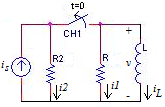
\includegraphics[scale=1.5]{RLN}
            \caption{Circuito RL}\label{RLN} 
        \end{figure} 
        
        Na resposta natural, o circuito RL funciona com a energia armazenada no indutor. No caso do circuito ser constituído por apenas um resistor e um indutor, após 10 constantes de tempo do circuito, não restará nenhuma energia armazenada no indutor.
        
Na análise é considerando o circuito da figura \ref{RLN}.

Condições iniciais do circuito antes de $t=0$:

\begin{itemize}
\item Chave fechada
\item Correntes e tensões constantes
\end{itemize}
        
Com as correntes constantes, o indutor se comporta como um curto-circuito, logo, toda a corrente $i_s$ da fonte passa pelo mesmo e a tensão em todos os elementos é igual a zero.

Em $t=0$, a chave $CH_1$ é aberta e, com isso, a fonte e o resistor $R_2$ são separados do resistor $R$ e indutor $L$. Estes últimos componentes constituem um circuito RL, apresentando resposta natural.

\begin{figure}[!htbp] \centering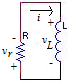
\includegraphics[scale=1.0]{RLN1}
            \caption{Circuito RL}\label{RLN1} 
        \end{figure} 

Após a abertura da chave, o indutor irá impor a corrente no circuito RL. Para analisar o mesmo, foram considerados os sentidos associados de corrente e tensão como mostrados na figura \ref{RLN1}.

A partir da LKT, considerando queda de tensão positiva e percorrendo o circuito no sentido da corrente:

\begin{equation}
v_R+v_L=0  \Rightarrow Ri+L\frac{di}{dt}=0
\end{equation}

\begin{equation}
\frac{di}{dt}=-\frac{R}{L}i
\end{equation}

\begin{equation}
\frac{di}{i}=-\frac{R}{L}dt
\end{equation}

Integrando ambos os termos:

\begin{equation}
\int\limits_{i(0)}^{i(t)}\frac{dy}{y} = \int\limits_{i(0)}^{t}-\frac{R}{L}dx \Rightarrow ln[i(t)]-ln[i(0)]=-\frac{R}{L} t \Rightarrow ln[\frac{i(t)}{i(0)}]= -\frac{R}{L} t
\end{equation}

\begin{equation}
\frac{i(t)}{i(0)} = e^{-\frac{R}{L} t}
\end{equation}

\begin{equation}
i(t) = i(0)e^{-\frac{R}{L} t}
\end{equation}

Considerando que $i(0) = i_s$:

\begin{equation}
i(t) = i_se^{-\frac{t}{\tau} t}
\end{equation}

Onde $\tau = \frac{L}{R}$, denominada de constante de tempo de um circuito RL.

\begin{remark}
Na resposta natural do circuito RL a constante de tempo determina o tempo de decaimento da corrente no indutor.
\end{remark}

\begin{remark}
Uma constante de tempo após o início de descarga do indutor, a corrente no circuito RL é reduzida a $e^{-1}$. Aproximadamente $37\%$ do valor inicial.
\end{remark}

\begin{remark}
Após cinco constantes de tempo, a corrente passa a ser menos que $1\%$ do valor inicial.
\end{remark}

        \begin{figure}[!htbp] \centering\includegraphics[scale=1.0]{energiaResidualRL}
            \caption{Circuito RL}\label{energiaResidualRL} 
        \end{figure}

\begin{remark}
Em um circuito RL contendo mais de um indutor, com pelo menos dois indutores conectados em paralelo, como apresentado na figura \ref{energiaResidualRL}, existe a possibilidade de que, em regime permanente, os indutores em paralelo armazenem uma energia residual. Para determinar se existirá energia residual, deve-se determinar o indutor equivalente da associação e sua energia inicial. Em seguida deve-se determinar a energia inicial do circuito. Para isso, calcula-se a energia individual de cada indutor e soma-se as mesmas. Se a energia inicial do circuito for maior que a energia inicial do indutor equivalente, haverá energia residual nos indutores conectados em paralelo. Só é possível haver energia residual em indutores associados em paralelo, pois os mesmos propiciam um caminho de circulação para a corrente, sem que esta passe por outro componente. Além disso, sendo a corrente constante, não será estabelecida qualquer tensão entre os terminais dos indutores, pois os mesmos estarão se comportando como um curto-circuito.
\end{remark}
        
        \subsection{Circuito RC}
        
        \begin{figure}[!htbp] \centering\includegraphics[scale=1.5]{RCN}
            \caption{Circuito RL}\label{RCN} 
        \end{figure} 
        
        Na resposta natural, o circuito RC funciona com a energia armazenada no capacitor. No caso do circuito ser constituído por apenas um resistor e um capacitor, após 10 constantes de tempo do circuito, não restará nenhuma energia armazenada no capacitor.
        
Na análise é considerando o circuito da figura \ref{RCN}.

Condições iniciais do circuito antes de $t=0$:

\begin{itemize}
\item Chave na posição A
\item Correntes e tensões constantes
\end{itemize}
        
Com as tensões constantes, o capacitor se comporta como um curto aberto, logo, a tensão $v_s$ da fonte é a mesma do capacitor e a corrente em todos os elementos é igual a zero.

Em $t=0$, a chave $CH_1$ muda para a posição B e, com isso, a fonte $v_s$ e o resistor $R_1$ são desligados. Neste instante o resistor $R$ e capacitor $C$ passam a formar um circuito RC, apresentando resposta natural.

\begin{figure}[!htbp] \centering\includegraphics[scale=1.0]{RCN1}
            \caption{Circuito RC}\label{RCN1} 
        \end{figure} 

Após a mudança da chave para a posição B, o capacitor irá impor a tensão no circuito RC, que provocará uma corrente que circulará por ambos os componentes. Para análise foram considerados os sentidos associados de corrente e tensão como mostrados na figura \ref{RCN1}.

A partir da LKC, considerando as correntes saindo do nó superior do circuito e que correntes saindo serão positivas, temos:

\begin{equation}
i_R+i_c=0  \Rightarrow \frac{v_c}{R}+C\frac{dv_c}{dt}=0
\end{equation}

\begin{equation}
\frac{dv_c}{dt}=-\frac{1}{RC}v_c
\end{equation}

\begin{equation}
\frac{dv_c}{v_c}=-\frac{1}{RC}dt
\end{equation}

Integrando ambos os termos:

\begin{equation}
\int\limits_{v_c(0)}^{v_c(t)}\frac{dy}{y} = \int\limits_{0}^{t}-\frac{1}{RC}dx \Rightarrow ln[v_c(t)]-ln[v_c(0)]=-\frac{1}{RC} t \Rightarrow ln[\frac{v_c(t)}{v_c(0)}]= -\frac{1}{RC} t
\end{equation}

\begin{equation}
\frac{v_c(t)}{v_c(0)} = e^{-\frac{1}{RC} t}
\end{equation}

\begin{equation}
v_c(t) = v_c(0)e^{-\frac{1}{RC} t}
\end{equation}

Considerando que $v_c(0) = v_s$:

\begin{equation}
v_c(t) = v_se^{-\frac{t}{\tau}}
\end{equation}

Onde $\tau = \frac{1}{RC}$, denominada de constante de tempo de um circuito RC.

\begin{remark}
Na resposta natural do circuito RC a constante de tempo determina o tempo de decaimento da tensão no capacitor.
\end{remark}

\begin{remark}
Uma constante de tempo após o início de descarga do capacitor, a tensão no circuito RC é reduzida a $e^{-1}$. Aproximadamente $37\%$ do valor inicial.
\end{remark}

\begin{remark}
Após cinco constantes de tempo, a tensão passa a ser menos que $1\%$ do valor inicial.
\end{remark}

        \begin{figure}[!htbp] \centering\includegraphics[scale=1.0]{energiaResidualRC}
            \caption{Circuito RC}\label{energiaResidualRC} 
        \end{figure}

\begin{remark}
Em um circuito RC contendo mais de um capacitor, com pelo menos dois capacitores conectados em série, como apresentado na figura \ref{energiaResidualRC}, existe a possibilidade de, em regime permanente, os capacitores em série armazenarem uma energia residual. Para determinar se existirá energia residual, deve-se determinar o capacitor equivalente da associação de capacitores e sua energia inicial. Em seguida deve-se determinar a energia inicial do circuito, para isso calcula-se a energia individual de cada capacitor e soma-se as mesmas. Se a energia inicial do circuito for maior que a energia inicial do capacitor equivalente, então haverá energia residual nos capacitores conectados em série. É possível haver energia em capacitores em série, pois caso os mesmo possuam tensões iguais e de polaridade invertida a tensão no circuito entre os terminais dos capacitores será nula. Além disso, sob tensão constante, capacitores se comportam como circuitos abertos.
\end{remark}
        
        
    
    \section{Resposta ao degrau}
    
        \subsection{Circuito RL}
        
        \begin{figure}[!htbp] \centering\includegraphics[scale=1.0]{RLD}
            \caption{Circuito RL}\label{RLD} 
        \end{figure}
        
Na resposta ao degrau, o circuito RL funciona com uma fonte de tensão e/ou corrente alimentando de forma permanente após um instante inicial. De maneira equivalente à resposta natural, após 10 constantes de tempo o circuito apresentará condições de regime permanente, ou seja, suas grandezas terão valores constantes.

Considerando o circuito apresentado na figura \ref{RLD}:

Condições iniciais do circuito antes de $t=0$:

\begin{itemize}
\item Chave aberta
\item Corrente nula
\end{itemize}

Em $t=0$, a chave $CH_1$ é fechada. Como a corrente inicial do indutor era zero, essa condição é mantida após o fechamento da chave, já que o indutor impede que a corrente mude instantaneamente. Dessa forma, toda a tensão da fonte é aplicada instantaneamente sobre o indutor.

Após o fechamento da chave em $t=0$ e usando a LKT, considerando queda de tensão positiva e percorrendo o circuito no sentido da corrente:

\begin{equation}
v_s=v_R+v_L=Ri+L\frac{di}{dt}
\end{equation}

\begin{equation}
\frac{di}{dt}=\frac{v_s}{L}-\frac{R}{L} i=-\frac{R}{L} (i-\frac{v_s}{R})
\end{equation}

\begin{equation}
\frac{di}{i-\frac{v_s}{R}} = -\frac{R}{L}dt
\end{equation}

Integrando ambos os termos:

\begin{equation}
\int\limits_{0}^{i(t)}\frac{di}{i-\frac{v_s}{R}} =\int\limits_{0}^{t} -\frac{R}{L}dt \Rightarrow ln[i(t)-\frac{v_s}{R}]-ln[i(0)-\frac{v_s}{R}]=-\frac{R}{L}t 
\end{equation}

\begin{equation}
ln[\frac{i(t)-\frac{v_s}{R}}{i(0)-\frac{v_s}{R}}] = -\frac{R}{L}t 
\end{equation}

\begin{equation}
\frac{i(t)-\frac{v_s}{R}}{i(0)-\frac{v_s}{R}} = e^{-\frac{R}{L}t}
\end{equation}

\begin{equation}
i(t) = \frac{v_s}{R} + [i(0)-\frac{v_s}{R}]e^{-\frac{t}{\tau}}
\end{equation}

Considerando que $i(0) = 0$:

\begin{equation}
i(t) = \frac{v_s}{R}(1-e^{-\frac{t}{\tau}})
\end{equation}

Onde $\tau=\frac{L}{R}$, denominada de constante de tempo de um circuito RL.

\begin{remark}
Na resposta ao degrau do circuito RL a constante de tempo determina o tempo de crescimento da corrente no indutor.
\end{remark}

\begin{remark}
Uma constante de tempo após o início de carga do indutor, a corrente no circuito RL é igual a $1-e^{-1}$. Aproximadamente $63\%$ do valor de regime permanente.
\end{remark}

\begin{remark}
Após cinco constantes de tempo, a corrente já atingiu mais de $99,3\%$ do valor de regime.
\end{remark}
        
        \subsection{Circuito RC}
        
                \begin{figure}[!htbp] \centering\includegraphics[scale=1.0]{RCD}
            \caption{Circuito RC}\label{RCD} 
        \end{figure}
        
Na resposta ao degrau o circuito RC funciona com uma fonte de tensão e/ou corrente alimentando o circuito de forma permanente, após um instante inicial. De forma equivalente a resposta natural, após 10 constantes de tempo o circuito apresentará condições de regime permanente, ou seja, suas grandezas terão valores constantes.

Considerando o circuito apresentado na figura \ref{RCD}:

Condições iniciais do circuito antes de $t=0$:

\begin{itemize}
\item Chave aberta
\item Tensão no capacitor nula
\end{itemize}

Em $t=0$, a chave $CH_1$ é fechada. Como a tensão inicial do capacitor era zero, essa condição é mantida após o fechamento da chave, já que o capacitor impede que a tensão mude instantaneamente. Dessa forma, toda a corrente da fonte é drenada pelo capacitor. Isso evita de passar qualquer corrente pelo resistor $R$, o que provocaria uma tensão em $t=0^+$ diferente de zero.

Após o fechamento da chave em t=0 e usando a LKC, considerando corrente saindo de um nó positiva e considerando o nó superior do circuito:

\begin{equation}
i_s=i_R+i_C=\frac{v_c}{R}+C\frac{dv_c}{dt}
\end{equation}

\begin{equation}
\frac{dv_c}{dt}=\frac{i_s}{C}-\frac{1}{RC} v_c=-\frac{1}{RC} (v_c-i_sR)
\end{equation}

\begin{equation}
\frac{dv_c}{v_c-i_sR} = -\frac{1}{RC}dt
\end{equation}

Integrando ambos os termos:

\begin{equation}
\int\limits_{v_c(0)}^{v_c(t)}\frac{dv_c}{v_c-i_sR} =\int\limits_{0}^{t} -\frac{1}{RC}dt \Rightarrow ln[v_c(t)-i_sR]-ln[v_c(0)-i_sR]=-\frac{1}{RC}t 
\end{equation}

\begin{equation}
ln[\frac{v_c(t)-i_sR}{v_c(0)-i_sR}] = -\frac{1}{RC}t 
\end{equation}

\begin{equation}
\frac{v_c(t)-i_sR}{v_c(0)-i_sR} = e^{-\frac{1}{RC}t}
\end{equation}

\begin{equation}
v_c(t) = i_sR + [v_c(0)-i_sR]e^{-\frac{t}{\tau}}
\end{equation}

Considerando que $v_c(0) = 0$:

\begin{equation}
v_c(t) = i_sR(1-e^{-\frac{t}{\tau}})
\end{equation}

Onde $\tau=\frac{1}{RC}$, denominada de constante de tempo de um circuito RC.

\begin{remark}
Na resposta ao degrau do circuito RC a constante de tempo determina o tempo de crescimento da tensão no capacitor.
\end{remark}

\begin{remark}
Uma constante de tempo após o início de carga do capacitor, a tensão no circuito RC é igual a $1-e^{-1}$. Aproximadamente $63\%$ do valor de regime permanente.
\end{remark}

\begin{remark}
Após cinco constantes de tempo, a tensão já atingiu mais de $99,3\%$ do valor de regime.
\end{remark}
     
    \section{Generalização da solução}
    
  \begin{figure}[!htbp] \centering\includegraphics[scale=1.0]{topologiaGeral}
            \caption{Topologias de circuitos de primeira ordem}\label{topologiaGeral} 
        \end{figure}    
    
    Circuitos de primeira ordem, do tipo RC ou RL, podem apresentar mais malhas do que os exemplos anteriormente apresentados. Nestes casos, caso seja possível minimizar os mesmos por meio de circuitos equivalentes Thévenin ou Norton, de modo que o circuito minimizado possa ser representado por alguma das topologias indicadas na figura \ref{topologiaGeral}, então é possível determinar a expressão de correntes e/ou tensões de capacitores e/ou indutores dos circuitos de primeira ordem através do uso da expressão geral:
    
    \begin{equation}
    x(t)=\lim_{\alpha\rightarrow\infty} x(\alpha)+[x(0)-\lim_{\alpha\rightarrow\infty}x(\alpha)] e^{-\frac{t}{\tau}}
    \end{equation}

Onde $x(t)$ é é a expressão no tempo de uma variável, corrente ou tensão, de interesse, $ \lim_{\alpha\rightarrow\infty}x(\alpha) $ é o valor de regime da variável selecionada, $x(0)$ é o valor inicial da variável selecionada e $\tau$ é a constante de tempo do circuito RL ou RC.

\begin{equation}
\left\{\begin{aligned} & 
        \text{(a)} &\frac{di}{dt}+\frac{i}{RC}=0\\& 
        \text{(b)} &\frac{dv}{dt}+\frac{R}{L}v=0\\&
        \text{(c)  } &\frac{di}{dt}+\frac{R}{L}i=\frac{v_{th}}{L}\\&
        \text{(d)  } &\frac{dv}{dt}+\frac{v}{RC}=\frac{i_N}{C}
    \end{aligned}\right.
\end{equation}

Equação diferencial geral:

\begin{equation}
\frac{dx}{dt} + \frac{x}{\tau} = k
\end{equation}

Como já discutido, após um período transitório, todas as grandezas dos circuitos de primeira ordem tendem para valores constantes no regime. Considerando isso, o termo $\frac{dx}{dt}$ da expressão geral tenderá para 0, logo, $\lim_{\alpha\rightarrow\infty}x(\alpha)=k\tau$.

Resolvendo a equação diferencial:

\begin{equation}
\frac{dx}{dt} = -\frac{x}{\tau} + k = -\frac{1}{\tau}(x-k\tau)
\end{equation}

\begin{equation}
\frac{dx}{x-k\tau} = -\frac{dt}{\tau}
\end{equation}

Integrando ambos os termos:

\begin{equation}
\int\limits_{x(0)}^{x(t)}\frac{dy}{y-k\tau} = \int\limits_{0}^{t}-\frac{du}{\tau}\Rightarrow ln[x(t)-k\tau]-ln[x(0)-k\tau] = -\frac{t}{\tau}
\end{equation}

\begin{equation}
ln[\frac{x(t)-k\tau}{x(0)-k\tau}] = -\frac{t}{\tau}
\end{equation}

\begin{equation}
\frac{x(t)-k\tau}{x(0)-k\tau} = e^{-\frac{t}{\tau}}\Rightarrow x(t) = k\tau + [x(0)-k\tau]e^{-\frac{t}{\tau}}
\end{equation}


Como $\lim_{\alpha\rightarrow\infty}x(\alpha)=k\tau$, então:

    \begin{equation}
    x(t)=\lim_{\alpha\rightarrow\infty}x(\alpha)+[x(0)-\lim_{\alpha\rightarrow\infty}x(\alpha)]e^{-\frac{t}{\tau}}
    \end{equation}
    
    \section{Resposta crescente}
    
\begin{figure}[!htbp] \centering\includegraphics[scale=1.0]{respostaCrescente}
            \caption{Circuito com resposta crescente}\label{respostaCrescente} 
        \end{figure}    
    
    Das analises anteriores observa-se que a resposta dos circuitos de primeira ordem, RC ou RL, tendem para condições de regime constante, que podem ser nulas ou não, dependendo do tipo de resposta, natural ou ao degrau, bem como das condições iniciais de energia dos capacitores ou indutores, como também da topologia dos circuitos. Esse comportamento, no entanto, pode ser alterado quando são utilizadas fontes de tensão e/ou correntes dependentes. Este tipo de fonte poderá definir uma resistência equivalente de Thévenin \textbf{"NEGATIVA"}. Caso isso se verifique, as constantes de tempo que compõem o expoente dos termos exponenciais e que forçam os respectivos termos a zero quando $t\rightarrow\infty$, não mais proporcionaram este decaimento e o circuito apresentará uma resposta \textbf{"CRESCENTE"}, como no caso do circuito da figura \ref{respostaCrescente} com o equivalente de Thévenin visto dos terminais do capacitor.  
        
     
%----------------------------------------------------------------------------------------
%	CHAPTER 10
%----------------------------------------------------------------------------------------
	
\chapterimage{includes/documents/chapter_head_2.pdf} % Chapter heading image
\chapter{Circuitos elétricos de segunda ordem}

Um circuito elétrico de segunda ordem é o tipo de circuito que tem sua dinâmica determinada por uma equação diferencial ordinária de segunda ordem.

\begin{equation}\label{segundaOrdemNatural}
\frac{d^2x(t)}{dt^2} + 2\zeta\omega_n\frac{dx(t)}{dt} + \omega_n^2x(t) = 0 
\end{equation}

\begin{equation}\label{segundaOrdemDegrau}
\frac{d^2x(t)}{dt^2} + 2\zeta\omega_n\frac{dx(t)}{dt} + \omega_n^2x(t) = x_f
\end{equation}

As equações escritas na forma de \ref{segundaOrdemNatural} e \ref{segundaOrdemDegrau} são utilizadas por padrão na teoria do controle moderno e facilitam a projeção de sistemas com respostas de segunda ordem. Esse controle é feito por meio da manipulação dos valores de $\zeta$ e $\omega$, que são dados em função dos parâmetros do circuito. Manipular os valores de $\zeta$ implicam numa manipulação direta no tempo em que o sistema entra em regime permanente, enquanto controlar os valores de $\omega$ permite modificar a quantidade de oscilações até a acomodação.

\section{Resposta natural}\label{desenvolvimento}
As expressões \ref{segundaOrdemNatural} e \ref{segundaOrdemDegrau} representam, respectivamente, as equações que definem o comportamento da resposta natural e ao degrau dos sistemas de segunda ordem.

Como $x(t)$ tem a característica de ser função de suas próprias derivadas, é possível considerar que $x(t) = Ae^{st}$ para se encontrar a solução para as equações.

Utilizando este artifício na equação \ref{segundaOrdemNatural}, vem:

\begin{equation}\label{natural}
\frac{d^2(Ae^{st})}{dt^2} + 2\zeta\omega_n\frac{d(Ae^{st})}{dt} + \omega_n^2Ae^{st} = 0
\end{equation}

\begin{equation}\label{d1}
\frac{d(Ae^{st})}{dt} = s(Ae^{st})
\end{equation}

\begin{equation}\label{d2}
\frac{d^2(Ae^{st})}{dt^2} = \frac{d(sAe^{st})}{dt} = s^2(Ae^{st})
\end{equation}

Substituindo \ref{d1} e \ref{d2} em \ref{natural}:

\begin{equation}
s^2(Ae^{st}) + 2\zeta\omega_ns(Ae^{st}) + \omega_n^2s^0(Ae^{st}) = 0
\end{equation}

Colocando $Ae^{st}$ em evidência:

\begin{equation}
Ae^{st}(s^2 + 2\zeta\omega_ns + \omega_n^2) = 0
\end{equation}

Como $Ae^{st} \neq 0$ :

\begin{equation}
s^2 + 2\zeta\omega_ns + \omega_n^2 = 0
\end{equation}

Desta forma :

\begin{equation}
s = \frac{-2\zeta\omega_n\pm\sqrt{(2\zeta\omega_n)^2-4\omega_n^2}}{2} = -\zeta\omega_n \pm \omega_n\sqrt{\zeta^2-1} = \omega_n(-\zeta\pm\sqrt{\zeta^2-1})
\end{equation}

\begin{equation}\label{s}
s = \omega_n(-\zeta\pm\sqrt{-1(-\zeta^2+1)}) = \omega_n(-\zeta\pm j\sqrt{1-\zeta^2})
\end{equation}

Como pode ser observado em \ref{s}, o tipo de resposta pode ter características diferentes quando contém ou não o termo imaginário, $j = \sqrt{-1}$, que a inclusão no valor de $s$ depende do valor de $\zeta$.

\subsection{Resposta superamortecida $1-\zeta^2 < 0$}

Nos casos em que $\zeta^2 > 1$, o valor de $j\sqrt{1-\zeta^2}$ é um número real negativo, pois $1-\zeta^2$ é um número negativo, o que acaba eliminando o termo imaginário da resposta. Assim:

\begin{equation}
s = -\zeta\omega_n \pm \omega_nj\sqrt{1-\zeta^2}
\end{equation}

Considerando $\alpha = \zeta\omega_n$ e $\beta = \omega_nj\sqrt{1-\zeta^2} < 0$:

\begin{equation}
s = -\alpha \pm \beta
\end{equation}

Obtendo o valor de $s$ e sabendo que este pode corresponder a dois números reais:

\begin{equation}\label{resultadoSuperamortecidoNatural}
x(t) = Ae^{st} \Rightarrow x(t) = A_1e^{(-\alpha + \beta)t} + A_2e^{(-\alpha - \beta)t}
\end{equation}

Com o resultado de \ref{resultadoSuperamortecidoNatural}, a dinâmica do sistema representa um decaimento exponencial se  $\alpha > 0$ e um crescimento exponencial se $\beta < \alpha < 0$.

\begin{remark}
O crescimento exponencial de uma grandeza implica em um crescimento de forma "descontrolada" da energia, o que é característica de um sistema \textbf{INSTÁVEL}.
\end{remark}

\begin{remark}
Os valores de $A$ e $-\alpha \pm \beta$ são determinados substituindo o valor de $x(t)$ na equação original e utilizando as condições iniciais do sistema.
\end{remark}

\subsection{Resposta criticamente amortecida $1-\zeta^2 = 0$}

Se $\zeta = \pm 1$, $s$ só tem um valor e é dado por $s = -\zeta\omega_n$. Com apenas um resultado possível para $s$, a solução seria dada por:

\begin{equation}\label{criticamenteAmortecida1}
x(t) = Ae^{-\zeta\omega_nt}
\end{equation}

O problema consiste na necessidade de duas equações para encontrar a resposta completa.

Derivando $Ae^{st}$ em relação à $s$, é possível obter a expressão necessária para completar a resposta.

\begin{equation}\label{criticamenteAmortecidaAuxiliar}
\frac{dAe^{st}}{ds} = Ate^{st}
\end{equation}

Com estas relações, a resposta passa a ser o conjunto de combinações lineares das expressões \ref{criticamenteAmortecida1} e \ref{criticamenteAmortecidaAuxiliar}:


\begin{equation}\label{resultadoCriticamenteAmortecidoNatural}
x(t) = A_1e^{-\alpha t} + A_2te^{-\alpha t}
\end{equation}

Onde $\alpha = \zeta\omega_n$.

Com o resultado de \ref{resultadoCriticamenteAmortecidoNatural}, se $\alpha > 0$, o sistema contém um decaimento exponencial e, no caso contrário, um crescimento exponencial.

\subsection{Resposta subamortecida $1-\zeta^2 > 0$}

Quando $1-\zeta^2 > 0$, $j\sqrt{1-\zeta^2}$ é um número complexo, pois $\sqrt{1-\zeta^2}$ é um número real.

Considerando $\alpha = \zeta\omega_n$ e $\omega = \omega_n\sqrt{1-\zeta^2}$:

\begin{equation}
s = -\alpha \pm j\omega
\end{equation}

\begin{equation}
x(t) = A_1e^{(-\alpha + j\omega)t} + A_2e^{(-\alpha - j\omega)t}
\end{equation}

\begin{equation}
x(t) = A_1e^{-\alpha t}e^{j\omega t} + A_2e^{-\alpha t}e^{-j\omega t}
\end{equation}

\begin{equation}
x(t) = e^{j\omega t}(A_1e^{-\alpha t}+ \frac{A_2}{e}e^{-\alpha t})
\end{equation}

\begin{equation}
x(t) = e^{j\omega t}(A_1+\frac{A_2}{e})e^{-\alpha t}
\end{equation}

Fazendo $A_1+\frac{A_2}{e} = D$:

\begin{equation}
x(t) = De^{-\alpha t}e^{j\omega t}
\end{equation}

Utilizando a relação de Euller:

\begin{equation}
e^{j\omega t} = cos(\omega t) + jsen(\omega t)
\end{equation}

\begin{equation}
x(t) = De^{-\alpha t}( cos(\omega t) + jsen(\omega t))
\end{equation}

\section{Resposta ao degrau}

Na resposta ao degrau, dada pela equação \ref{segundaOrdemDegrau}, uma das soluções é considerar $x(t) = A$. Assim:

\begin{equation}
\frac{dx(t)}{dt} = \frac{dA}{dt} = 0
\end{equation}

\begin{equation}
\frac{d^2x(t)}{dt^2} = \frac{d0}{dt} = 0
\end{equation}

Substituindo em \ref{segundaOrdemDegrau} :

\begin{equation}
0 + 2\zeta\omega_n0 + \omega_n^2A = x_f \Rightarrow A = \frac{x_f}{\omega_n^2}
\end{equation}

Desta forma, a solução é dada por combinações lineares de uma constante e da resposta dada pela resposta natural do sistema.

Considerando os desenvolvimentos dos tipos de respostas já obtidos para a resposta natural, é possível sistematizar as respostas do sistema submetido a um degrau nas subseções que seguem:

\subsection{Resposta superamortecida}
\begin{equation}
x(t) = A_1e^{(-\alpha + \beta)t} + A_2e^{(-\alpha - \beta)t} + A_3
\end{equation}

\subsection{Resposta criticamente amortecida}
\begin{equation}
x(t) = A_1e^{-\alpha t} + A_2te^{-\alpha t} + A_3
\end{equation}

\subsection{Resposta subamortecida}
\begin{equation}
x(t) = De^{-\alpha t}( cos(\omega t) + jsen(\omega t)) + A
\end{equation}

\section{Circuito RLC paralelo}
        
        \subsection{Resposta natural}
        
\begin{figure}[!htbp]\centering
\begin{circuitikz}
\draw
(0,2)to(2,2)to(4,2)
(0,0)to(2,0)to(4,0)

(0,0) to[R=$R$, i=$i_R$](0,2)
(2,0) to[cute inductor=$L$, i=$i_L$](2,2)
(4,0) to[C=$C$, v>=$v_c$, i=$i_c$](4,2)
;
\end{circuitikz}
\caption{Circuito RLC em paralelo}
\end{figure}\label{RLCNatural}

Aplicando a LKC no circuito da figura \ref{RLCNatural}, é possível observar que:

\begin{equation}
i_c + i_R + i_L = 0
\end{equation}

\begin{equation}
\left\{\begin{aligned} & 
        i_R = \frac{v_c}{R}\\& 
        i_c = C\frac{dv_c}{dt}\\&        
        i_L = \frac{1}{L}\int v_cdt
    \end{aligned}\right.
\end{equation}

\begin{equation}
C\frac{dv_c}{dt} + \frac{v_c}{R} + \frac{1}{L}\int v_cdt = 0
\end{equation}

Derivando ambos os membros em relação ao tempo, obtém-se uma equação diferencial ordinária de segunda ordem:

\begin{equation}
C\frac{d^2v_c}{dt^2} + \frac{1}{R}\frac{dv_c}{dt} + \frac{1}{L} v_c = 0
\end{equation}

\begin{equation}
\frac{d^2v_c}{dt^2} + \frac{1}{RC}\frac{dv_c}{dt} + \frac{1}{LC} v_c = 0
\end{equation}

Fazendo $\omega_n^2 = \frac{1}{LC}$ e $2\zeta\omega_n = \frac{1}{RC}$, vem:

\begin{equation}
\frac{d^2v_c(t)}{dt^2} + 2\zeta\omega_n\frac{dv_c(t)}{dt} + \omega_n^2v_c(t) = 0
\end{equation}

\begin{equation}
\omega_n = \frac{1}{\sqrt{LC}}
\end{equation}

\begin{equation}
\zeta = \frac{\sqrt{LC}}{2RC}
\end{equation}

        
            \subsubsection{Superamortecida}

Para o circuito apresentar uma resposta superamortecida, $1-\zeta^2 < 0$. Isso implica nas seguintes relações:

\begin{equation}
1-\zeta^2 < 0 \Rightarrow \frac{L}{4R^2C} > 1 \Rightarrow L > 4R^2C \Rightarrow \frac{L}{R} > 4RC
\end{equation}

Satisfeitas as condições, a resposta de $v_c(t)$ pode ser dada por:

\begin{equation}
v_c(t) = A_1e^{(-\alpha + \beta)t} + A_2e^{(-\alpha - \beta)t}
\end{equation}

Onde $\alpha = \zeta\omega_n$ e $\beta = \omega_n\sqrt{\zeta^2-1}$.

\begin{equation}
\left\{\begin{aligned} & 
        \alpha = \frac{1}{2RC}\\&         
        \beta = \sqrt{\frac{1}{4R^2C^2}-\frac{1}{LC}} = \sqrt{\alpha^2-\omega_n^2}
    \end{aligned}\right.
\end{equation}

Para determinar os valore de $A_1$ e $A_2$, é necessário o conhecimento dos valores iniciais de tensão e corrente no capacitor. Considerando $i_c(0) = i$ e $v_c(0) = v$, vem:

\begin{equation}
v_c(0) = v = A_1e^{(-\alpha + \beta)0} + A_2e^{(-\alpha - \beta)0}
\end{equation}

\begin{equation}
v = A_1 + A_2
\end{equation}

\begin{equation}
C\frac{dv_c(t)}{dt} = i_c(t) = C(-\alpha + \beta)A_1e^{(-\alpha + \beta)t} + C(-\alpha - \beta)A_2e^{(-\alpha - \beta)t}
\end{equation}

\begin{equation}
C\frac{dv_c(0)}{dt} = i =  C(-\alpha + \beta)A_1e^{(-\alpha + \beta)0} + C(-\alpha - \beta)A_2e^{(-\alpha - \beta)0}
\end{equation}

\begin{equation}
i = C(-\alpha + \beta)A_1 + C(-\alpha - \beta)A_2
\end{equation}

O que resulta no sistema:

\begin{equation}
\begin{bmatrix}
1 & 1\\
C(-\alpha + \beta) & C(-\alpha - \beta)
\end{bmatrix}
\begin{bmatrix}
A_1\\A_2
\end{bmatrix}
=
\begin{bmatrix}
 v\\i
\end{bmatrix}
\end{equation}

\begin{equation}
\begin{bmatrix}
A_1\\A_2
\end{bmatrix}
=-\frac{1}{2C\beta}
\begin{bmatrix}
C(-\alpha - \beta) & 1\\
-C(-\alpha + \beta) & -1
\end{bmatrix}
\begin{bmatrix}
 v_c(0)\\i_c(0)
\end{bmatrix}
\end{equation}

Uma vez determinados as expressões para tensão e corrente no capacitor, as grandezas dos dois outros componentes é dada na forma que segue:

\begin{equation}
\left\{\begin{aligned} & 
        i_R(t) = \frac{v_c(t)}{R}\\&       
        i_L(t) = -(i_R(t) + i_c(t))
    \end{aligned}\right.
\end{equation}

            
            \subsubsection{Criticamente amortecida}
            
Para o circuito apresentar uma resposta criticamente amortecida, $1-\zeta^2 = 0$. Isso implica nas seguintes relações:

\begin{equation}
1-\zeta^2 = 0 \Rightarrow \frac{L}{4R^2C} = 1 \Rightarrow L = 4R^2C \Rightarrow \frac{L}{R} = 4RC
\end{equation}

Satisfeitas as condições, a resposta de $v_c(t)$ pode ser dada por:

\begin{equation}
v_c(t) = A_1e^{-\alpha t} + A_2te^{-\alpha t}
\end{equation}

Onde $\alpha = \zeta\omega_n = \frac{1}{2RC}$. 

Sabendo as condições iniciais do capacitor , $v_c(0) = v$ e $i_c(0) = i$, vem:

\begin{equation}
v_c(0) = v = A_1e^{-\alpha 0} + A_20e^{-\alpha 0}
\end{equation}

\begin{equation}
v = A_1
\end{equation}

\begin{equation}
C\frac{dv_c(t)}{dt} = i_c(t) = -C\alpha A_1e^{-\alpha t}  -C\alpha tA_2te^{-\alpha t} + CA_2e^{-\alpha t}
\end{equation}

\begin{equation}
C\frac{dv_c(0)}{dt} = i = -C\alpha A_1e^{-\alpha 0}  -C\alpha tA_20e^{-\alpha 0} + CA_2e^{-\alpha 0}
\end{equation}

\begin{equation}
i = -C\alpha A_1 + CA_2 \Rightarrow A_2 = \frac{i_c(0)}{C}+\alpha v_c(0)
\end{equation}
            
            
            \subsubsection{Subamortecida}

Para o circuito apresentar uma subamortecida, $1-\zeta^2 > 0$. Isso implica nas seguintes relações:

\begin{equation}
1-\zeta^2 > 0 \Rightarrow \frac{L}{4R^2C} <1 1 \Rightarrow L < 4R^2C \Rightarrow \frac{L}{R} < 4RC
\end{equation}

Satisfeitas as condições, a resposta de $v_c(t)$ pode ser dada por:

\begin{equation}
v_c(t) = De^{-\alpha t}( cos(\omega t) + jsen(\omega t))
\end{equation}

Onde $\alpha = \zeta\omega_n = \frac{1}{2RC}$ e $\omega = \omega_n\sqrt{1-\zeta^2} = \sqrt{\frac{1}{LC}-\frac{1}{4R^2C^2}}$

Com o valor inicial da tensão, $v_c(0) = v$, vem:

\begin{equation}
v_c(0) = v = De^{-\alpha 0}( cos(\omega 0) + jsen(\omega 0)) \Rightarrow D = v = v_c(0)
\end{equation}

\begin{equation}
\frac{dv_c(t)}{dt} = -\alpha v_c(t) + De^{-\alpha t}( -\omega sen(\omega t) + j\omega cos(\omega t))
\end{equation}


\begin{equation}
i_c(t) = -C\alpha De^{-\alpha t}( cos(\omega t) + jsen(\omega t)) + CDe^{-\alpha t}( -\omega sen(\omega t) + j\omega cos(\omega t))
\end{equation}

\begin{equation}
i_c(t) = Cv_c(0)e^{-\alpha t}[(-\alpha+j\omega)cos(\omega t)+(-\omega-j\alpha)sen(\omega t)]
\end{equation}

        
        \subsection{Resposta ao degrau}
        
\begin{figure}[!htbp]\centering
\begin{circuitikz}
\draw
(0,2)to(2,2)to(4,2)to(6,2)to(8,2)
(0,0)to(2,0)to(4,0)to(6,0)to(8,0)

(2,0) to[ospst=$CH_1$]              (2,2)

(0,0) to[I=$i_s$]                   (0,2)
(4,0) to[R=$R$, i<=$i_R$]            (4,2)
(6,0) to[cute inductor=$L$, i<=$i_L$](6,2)
(8,0) to[C=$C$, v>=$v_c$, i<=$i_c$]  (8,2)
;
\end{circuitikz}
\caption{Circuito RLC em paralelo}
\end{figure}\label{RLCDegrau}   

Aplicando a LKC no circuito da figura \ref{RLCDegrau} após a abertura da chave:

\begin{equation}
i_c + i_R + i_L = i_s
\end{equation}

\begin{equation}
\left\{\begin{aligned} & 
        i_R = \frac{v_c}{R}\\& 
        i_c = C\frac{dv_c}{dt}\\&        
        i_L = \frac{1}{L}\int v_cdt
    \end{aligned}\right.
\end{equation}

\begin{equation}
C\frac{dv_c}{dt} + \frac{v_c}{R} + \frac{1}{L}\int v_cdt = i_s
\end{equation}

Derivando ambos os membros em relação ao tempo, obtém-se uma equação diferencial ordinária de segunda ordem:

\begin{equation}
C\frac{d^2v_c}{dt^2} + \frac{1}{R}\frac{dv_c}{dt} + \frac{1}{L} v_c = 0
\end{equation}

\begin{equation}
\frac{d^2v_c}{dt^2} + \frac{1}{RC}\frac{dv_c}{dt} + \frac{1}{LC} v_c = 0
\end{equation}   

O que mostra que a dinâmica do circuito é a mesma da resposta natural. A diferença consiste nos valores finais das grandezas. No caso da resposta natural, todas as grandezas tendiam a um valor nulo no regime permanente. Na resposta ao degrau, o valor médio da corrente no circuito é uma constante mesmo depois do transitório.

Como a dinâmica do circuito é a mesma, os critérios considerados e os resultados obtidos no caso da resposta natural podem ser utilizados para determinar os valores na resposta ao degrau.
        
            \subsubsection{Superamortecida}
            
\begin{equation}
\left\{\begin{aligned} & 
        v_c(t) = A_1e^{(-\alpha + \beta)t} + A_2e^{(-\alpha - \beta)t} + v_{c_f}\\&       
        i_c(t) = B_1e^{(-\alpha + \beta)t} + B_2e^{(-\alpha - \beta)t} + i_{c_f}
    \end{aligned}\right.
\end{equation}

\begin{equation}
\left\{\begin{aligned} & 
        v_L(t) = C_1e^{(-\alpha + \beta)t} + C_2e^{(-\alpha - \beta)t} + v_{L_f}\\&       
        i_L(t) = D_1e^{(-\alpha + \beta)t} + D_2e^{(-\alpha - \beta)t} + i_{L_f}
    \end{aligned}\right.
\end{equation}

\begin{equation}
\left\{\begin{aligned} & 
        v_R(t) = E_1e^{(-\alpha + \beta)t} + E_2e^{(-\alpha - \beta)t} + v_{R_f}\\&       
        i_R(t) = F_1e^{(-\alpha + \beta)t} + F_2e^{(-\alpha - \beta)t} + i_{R_f}
    \end{aligned}\right.
\end{equation}
            
            \subsubsection{Criticamente amortecida}

\begin{equation}
\left\{\begin{aligned} & 
        v_R(t) = A_1e^{-\alpha t} + A_2te^{-\alpha t} + v_{R_f}\\&       
        i_R(t) = B_1e^{-\alpha t} + B_2te^{-\alpha t} + i_{R_f}
    \end{aligned}\right.
\end{equation}  

\begin{equation}
\left\{\begin{aligned} & 
        v_L(t) = C_1e^{-\alpha t} + C_2te^{-\alpha t} + v_{L_f}\\&       
        i_L(t) = D_1e^{-\alpha t} + D_2te^{-\alpha t} + i_{L_f}
    \end{aligned}\right.
\end{equation}

\begin{equation}
\left\{\begin{aligned} & 
        v_C(t) = E_1e^{-\alpha t} + E_2te^{-\alpha t} + v_{c_f}\\&       
        i_C(t) = F_1e^{-\alpha t} + F_2te^{-\alpha t} + i_{c_f}
    \end{aligned}\right.
\end{equation}          
            
            \subsubsection{Subamortecida}

\begin{equation}
\left\{\begin{aligned} & 
        v_L(t) = Ae^{-\alpha t}( cos(\omega t) + jsen(\omega t)) + v_{L_f}\\&       
        i_L(t) = Be^{-\alpha t}( cos(\omega t) + jsen(\omega t)) + i_{L_f}
    \end{aligned}\right.
\end{equation}

\begin{equation}
\left\{\begin{aligned} & 
        v_C(t) = De^{-\alpha t}( cos(\omega t) + jsen(\omega t)) + v_{c_f}\\&       
        i_C(t) = Ee^{-\alpha t}( cos(\omega t) + jsen(\omega t)) + i_{c_f}
    \end{aligned}\right.
\end{equation}

\begin{equation}
\left\{\begin{aligned} & 
        v_R(t) = Fe^{-\alpha t}( cos(\omega t) + jsen(\omega t)) + v_{R_f}\\&       
        i_R(t) = Ge^{-\alpha t}( cos(\omega t) + jsen(\omega t)) + i_{R_f}
    \end{aligned}\right.
\end{equation}
            
    \section{Circuito RLC série}

\begin{figure}[!htbp]\centering
\begin{circuitikz}
\draw
(0,2)to[R=$R$, v=$v_R$](2,2)to[cute inductor=$L$, v=$v_L$](4,2)
(0,0)to(2,0)to(4,0)
(0,0) to[short, i=$i$](0,2)
(4,0) to[C=$C$, v>=$v_c$,](4,2)
;
\end{circuitikz}
\caption{Circuito RLC em série}
\end{figure}\label{RLCNatural}

Aplicando LKT no circuito da figura \ref{RLCNatural}:

\begin{equation}
v_L + v_R + v_c = 0
\end{equation} 

\begin{equation}
L\frac{di(t)}{dt} + Ri(t) + \frac{1}{C}\int i(t)dt = 0
\end{equation}

Derivando em relação ao tempo:

\begin{equation}
L\frac{d^2i(t)}{dt^2} + R\frac{di(t)}{dt} + \frac{1}{C}i(t) = 0
\end{equation}

\begin{equation}
\frac{d^2i(t)}{dt^2} + \frac{R}{L}\frac{di(t)}{dt} + \frac{1}{LC}i(t) = 0
\end{equation}

Fazendo $\zeta\omega_n = \frac{R}{2L}$ e $\omega_n^2 = \frac{1}{LC}$:

\begin{equation}
\frac{d^2i(t)}{dt^2} + 2\zeta\omega_n\frac{di(t)}{dt} + \omega_n^2i(t) = 0
\end{equation}

Onde $\alpha = \zeta\omega_n$ e $\beta = \omega_n\sqrt{\zeta^2-1}$.

As respostas para essa equação já foram determinadas na seção \ref{desenvolvimento}.

    
        \subsection{Resposta natural}
            
            \subsubsection{Superamortecida}
            

\begin{equation}
\left\{\begin{aligned} & 
        \alpha = \frac{R}{2L}\\&         
        \beta = \sqrt{\frac{R^2}{4L^2}-\frac{1}{LC}} = \sqrt{\alpha^2-\omega_n^2}
    \end{aligned}\right.
\end{equation}
            
\begin{equation}
\left\{\begin{aligned} & 
        v_c(t) = A_1e^{(-\alpha + \beta)t} + A_2e^{(-\alpha - \beta)t} \\&       
        i_c(t) = B_1e^{(-\alpha + \beta)t} + B_2e^{(-\alpha - \beta)t} 
    \end{aligned}\right.
\end{equation}

\begin{equation}
\left\{\begin{aligned} & 
        v_L(t) = C_1e^{(-\alpha + \beta)t} + C_2e^{(-\alpha - \beta)t} \\&       
        i_L(t) = D_1e^{(-\alpha + \beta)t} + D_2e^{(-\alpha - \beta)t} 
    \end{aligned}\right.
\end{equation}

\begin{equation}
\left\{\begin{aligned} & 
        v_R(t) = E_1e^{(-\alpha + \beta)t} + E_2e^{(-\alpha - \beta)t} \\&       
        i_R(t) = F_1e^{(-\alpha + \beta)t} + F_2e^{(-\alpha - \beta)t} 
    \end{aligned}\right.
\end{equation}
            
            \subsubsection{Criticamente amortecida}

\begin{equation}
\left\{\begin{aligned} & 
        v_R(t) = A_1e^{-\alpha t} + A_2te^{-\alpha t} \\&       
        i_R(t) = B_1e^{-\alpha t} + B_2te^{-\alpha t} 
    \end{aligned}\right.
\end{equation}  

\begin{equation}
\left\{\begin{aligned} & 
        v_L(t) = C_1e^{-\alpha t} + C_2te^{-\alpha t} \\&       
        i_L(t) = D_1e^{-\alpha t} + D_2te^{-\alpha t} 
    \end{aligned}\right.
\end{equation}

\begin{equation}
\left\{\begin{aligned} & 
        v_C(t) = E_1e^{-\alpha t} + E_2te^{-\alpha t} \\&       
        i_C(t) = F_1e^{-\alpha t} + F_2te^{-\alpha t} 
    \end{aligned}\right.
\end{equation}          
            
            \subsubsection{Subamortecida}
            

$\alpha = \zeta\omega_n = \frac{R}{2L}$ e $\omega = \omega_n\sqrt{1-\zeta^2} = \sqrt{\frac{1}{LC}-\frac{R^2}{4L^2}}$

\begin{equation}
\left\{\begin{aligned} & 
        v_L(t) = Ae^{-\alpha t}( cos(\omega t) + jsen(\omega t))\\&       
        i_L(t) = Be^{-\alpha t}( cos(\omega t) + jsen(\omega t))
    \end{aligned}\right.
\end{equation}

\begin{equation}
\left\{\begin{aligned} & 
        v_C(t) = De^{-\alpha t}( cos(\omega t) + jsen(\omega t)) \\&       
        i_C(t) = Ee^{-\alpha t}( cos(\omega t) + jsen(\omega t))
    \end{aligned}\right.
\end{equation}

\begin{equation}
\left\{\begin{aligned} & 
        v_R(t) = Fe^{-\alpha t}( cos(\omega t) + jsen(\omega t)) \\&       
        i_R(t) = Ge^{-\alpha t}( cos(\omega t) + jsen(\omega t))
    \end{aligned}\right.
\end{equation}
        
        \subsection{Resposta ao degrau}
        
        \begin{figure}[!htbp]\centering
\begin{circuitikz}
\draw
(0,2)to[R=$R$, v=$v_R$](2,2)to[cute inductor=$L$, v=$v_L$](4,2)
(0,0)to(2,0)to(4,0)
(0,0) to[V=$v_s$, i=$i$](0,2)
(4,0) to[C=$C$, v>=$v_c$,](4,2)
;
\end{circuitikz}
\caption{Circuito RLC em série}
\end{figure}\label{RLCDegrau}

Aplicando a LKT no circuito da figura \ref{RLCDegrau}:

\begin{equation}
v_L + v_R + v_c = v_s
\end{equation} 

\begin{equation}
L\frac{di(t)}{dt} + Ri(t) + \frac{1}{C}\int i(t)dt = v_s
\end{equation}

Derivando em relação ao tempo:

\begin{equation}
L\frac{d^2i(t)}{dt^2} + R\frac{di(t)}{dt} + \frac{1}{C}i(t) = 0
\end{equation}

\begin{equation}
\frac{d^2i(t)}{dt^2} + \frac{R}{L}\frac{di(t)}{dt} + \frac{1}{LC}i(t) = 0
\end{equation}

Fazendo $\zeta\omega_n = \frac{R}{2L}$ e $\omega_n^2 = \frac{1}{LC}$:

\begin{equation}
\frac{d^2i(t)}{dt^2} + 2\zeta\omega_n\frac{di(t)}{dt} + \omega_n^2i(t) = 0
\end{equation}

Onde $\alpha = \zeta\omega_n$ e $\beta = \omega_n\sqrt{\zeta^2-1}$.

As respostas para essa equação já foram determinadas na seção \ref{desenvolvimento}.


            \subsubsection{Superamortecida}
            
            \begin{equation}
\left\{\begin{aligned} & 
        \alpha = \frac{R}{2L}\\&         
        \beta = \sqrt{\frac{R^2}{4L^2}-\frac{1}{LC}} = \sqrt{\alpha^2-\omega_n^2}
    \end{aligned}\right.
\end{equation}

\begin{equation}
\left\{\begin{aligned} & 
        v_c(t) = A_1e^{(-\alpha + \beta)t} + A_2e^{(-\alpha - \beta)t} + v_{c_f}\\&       
        i_c(t) = B_1e^{(-\alpha + \beta)t} + B_2e^{(-\alpha - \beta)t} + i_{c_f}
    \end{aligned}\right.
\end{equation}

\begin{equation}
\left\{\begin{aligned} & 
        v_L(t) = C_1e^{(-\alpha + \beta)t} + C_2e^{(-\alpha - \beta)t} + v_{L_f}\\&       
        i_L(t) = D_1e^{(-\alpha + \beta)t} + D_2e^{(-\alpha - \beta)t} + i_{L_f}
    \end{aligned}\right.
\end{equation}

\begin{equation}
\left\{\begin{aligned} & 
        v_R(t) = E_1e^{(-\alpha + \beta)t} + E_2e^{(-\alpha - \beta)t} + v_{R_f}\\&       
        i_R(t) = F_1e^{(-\alpha + \beta)t} + F_2e^{(-\alpha - \beta)t} + i_{R_f}
    \end{aligned}\right.
\end{equation}
            
            \subsubsection{Criticamente amortecida}

\begin{equation}
\left\{\begin{aligned} & 
        v_R(t) = A_1e^{-\alpha t} + A_2te^{-\alpha t} + v_{R_f}\\&       
        i_R(t) = B_1e^{-\alpha t} + B_2te^{-\alpha t} + i_{R_f}
    \end{aligned}\right.
\end{equation}  

\begin{equation}
\left\{\begin{aligned} & 
        v_L(t) = C_1e^{-\alpha t} + C_2te^{-\alpha t} + v_{L_f}\\&       
        i_L(t) = D_1e^{-\alpha t} + D_2te^{-\alpha t} + i_{L_f}
    \end{aligned}\right.
\end{equation}

\begin{equation}
\left\{\begin{aligned} & 
        v_C(t) = E_1e^{-\alpha t} + E_2te^{-\alpha t} + v_{c_f}\\&       
        i_C(t) = F_1e^{-\alpha t} + F_2te^{-\alpha t} + i_{c_f}
    \end{aligned}\right.
\end{equation}          
            
            \subsubsection{Subamortecida}


$\alpha = \zeta\omega_n = \frac{R}{2L}$ e $\omega = \omega_n\sqrt{1-\zeta^2} = \sqrt{\frac{1}{LC}-\frac{R^2}{4L^2}}$

\begin{equation}
\left\{\begin{aligned} & 
        v_L(t) = Ae^{-\alpha t}( cos(\omega t) + jsen(\omega t)) + v_{L_f}\\&       
        i_L(t) = Be^{-\alpha t}( cos(\omega t) + jsen(\omega t)) + i_{L_f}
    \end{aligned}\right.
\end{equation}

\begin{equation}
\left\{\begin{aligned} & 
        v_C(t) = De^{-\alpha t}( cos(\omega t) + jsen(\omega t)) + v_{c_f}\\&       
        i_C(t) = Ee^{-\alpha t}( cos(\omega t) + jsen(\omega t)) + i_{c_f}
    \end{aligned}\right.
\end{equation}

\begin{equation}
\left\{\begin{aligned} & 
        v_R(t) = Fe^{-\alpha t}( cos(\omega t) + jsen(\omega t)) + v_{R_f}\\&       
        i_R(t) = Ge^{-\alpha t}( cos(\omega t) + jsen(\omega t)) + i_{R_f}
    \end{aligned}\right.
\end{equation}
    
    \section{Superposição}
    
    Quando o circuito a ser analisado apresenta mais de uma fonte de alimentação, sua análise pode ser realizada considerando a ação conjunta de todas as fontes, ou a partir do método da superposição. É possível analisar circuitos lineares invariantes no tempo considerando a ação isolada de cada fonte de alimentação e por fim, realizando a soma das componentes das grandezas calculadas. Como os circuitos de primeira e segunda ordem atendem aos requisitos de linearidade e invariância no tempo (componentes não alteram suas características ao longo do tempo), então a aplicação do método da superposição é possível na análise desses circuitos.

Ao usar o método da superposição na análise dos circuitos de primeira e segunda ordem, deve-se atentar para o fato de que \textbf{as condições iniciais de capacitores e/ou indutores só podem ser consideradas uma única vez ao desmembrar a análise em várias sub-análises}, de acordo com o número de fontes existentes no circuito.
        
    
    \section{Fator de qualidade}
    
Por definição: $Q=\frac{\omega_n}{2\alpha}$

Circuito RLC paralelo: $Q=\frac{RC}{\sqrt{LC}}$

Circuito RLC Série: $Q=\frac{L}{R\sqrt{LC}}$

O fator de qualidade indica o nível de amortecimento de um circuito RLC. Quanto menor o amortecimento, maior o valor de Q. No limite, quando o amortecimento tende a 0, Q tende a infinito.

O fator de qualidade também pode ser interpretado em termos de energia. Nesta interpretação, o fator de qualidade representa a relação entre a energia que é transferida de um elemento armazenador para outro (capacitor$\rightarrow$indutor e vice-versa) e a energia que é dissipada nesta transferência. Como o tempo de observação é o mesmo, a relação pode ser dada em termos da potência reativa, que representa a energia transferida e a potência média ativa, que representa a energia dissipada. Quanto menor o valor da potência dissipada para um mesmo valor de potência reativa, maior o fator Q.
$$Q=\frac{\text{Potência reativa}}{\text{Potência ativa média}}$$

}             
%----------------------------------------------------------------------------------------
%	PART
%----------------------------------------------------------------------------------------

\part{Terceiro Estágio}

%----------------------------------------------------------------------------------------
%	CHAPTER 10
%----------------------------------------------------------------------------------------
	
\chapterimage{includes/documents/chapter_head_2.pdf} % Chapter heading image
\chapter{Sinais elétricos}

Sinal é um termo que deriva do latim \textit{signalis} e corresponde a um conjunto de informações. Os sinais elétricos são formados por variações de tensão ou corrente. Essas variações podem ser na amplitude, forma de onda, frequencia ou qualquer outra propriedade mensurável que a criatividade humana permita. Utilizados na codificação, decodificação e transmissão de informações, não só nas telecomunicações, mas em todas as demais áreas de conhecimento da engenharia elétrica, os sinais desempenham um trabalho fundamental na aquisição de dados e acionamento de componentes. Embora operem com baixa potência, em geral, os sinais também são muito utilizados nos equipamentos elétricos de alta potência com o auxílio e avanço das técnicas empregadas na eletrônica de potência.

   \section{Função degrau {$u(t)$}}
   
   \begin{figure}[!htbp] \centering\includegraphics[scale=1.0]{degrau}
            \caption{Função degrau $u(t)$}\label{degrau} 
        \end{figure} 

A função $f(t)$ na imagem \ref{degrau} é denominada de função degrau, a qual se caracteriza por uma transição (descontinuidade da curva) em um dado instante t. No caso indicado no gráfico, a transição ocorre em $t=0$. Caso o valor de $k$ seja igual a $1$, então a função recebe a denominação de função degrau unitário, sendo representada por $u(t)$.

\begin{equation}\label{u(t)}
f(t) =\left\{\begin{aligned}  & 
        0,&\text{se }t<0\\&       
        ku(t) = k,&\text{se }t>0
    \end{aligned}\right.
\end{equation}

\begin{figure}[!htbp] \centering\includegraphics[scale=1.0]{degrauLinear}
            \caption{Função degrau $u(t)$}\label{degrauLinear} 
        \end{figure}

É importante observar que a função \ref{u(t)} não é definida em 0. Embora a função degrau não seja definida em $t=0$, sob determinadas condições pode-se definir a mesma entre os instantes $\varepsilon^-$ e $\varepsilon^+$, com $\varepsilon\rightarrow0$, como uma função linear, como pode ser visto na figura \ref{degrauLinear}. 

\begin{equation}\label{u(t)}
f(t) =\left\{\begin{aligned}  & 
        0,&\text{se }t<\varepsilon^-\\&       
        ku(t) = k,&\text{se }t>\varepsilon^+\\&
        k(0,5+\frac{t}{2\varepsilon})&\text{se }\varepsilon^-<t<\varepsilon^+
    \end{aligned}\right.
\end{equation} 

\begin{figure}[!htbp] \centering\includegraphics[scale=1.0]{degrauDeslocado}
            \caption{Função degrau $u(t)$}\label{degrauDeslocado} 
        \end{figure}

A função degrau pode apresentar instantes de transição diferentes de $t=0$, neste caso, as mesmas são representadas graficamente como na figura \ref{degrauDeslocado}.

\begin{equation}\label{u(t)}
\text{(a) }f(t) =\left\{\begin{aligned}  & 
        0,&\text{se }t<a\\&       
        ku(t-a) = k,&\text{se }t>a
    \end{aligned}\right.
\end{equation}

\begin{equation}\label{u(t)}
\text{(b) }f(t) =\left\{\begin{aligned}  & 
        0,&\text{se }t<-a\\&       
        ku(t+a) = k,&\text{se }t>-a
    \end{aligned}\right.
\end{equation}

A função degrau fornece valores diferentes de zero sempre que seu argumento é maior que zero. Esse tipo de função pode ser utilizado para representar funções com pulsos.

\begin{figure}[!htbp] \centering\includegraphics[scale=1.0]{pulso1}
            \caption{Função degrau $u(t)$}\label{pulso1} 
        \end{figure}
        \begin{figure}[!htbp] \centering\includegraphics[scale=1.0]{pulso2}
            \caption{Função degrau $u(t)$}\label{pulso2} 
        \end{figure}

Pode ser mostrado que a função pulso $f(t)$ na figura \ref{pulso1} pode ser representada pela soma das seguintes funções degrau:

\begin{equation}
u_1 (t)=3u(t-(-3))=3u(t+3)
\end{equation}

\begin{equation}
u_2 (t)=6u(t-1)
\end{equation}

\begin{equation}
u_3 (t)=5u(t-4)
\end{equation}

\begin{equation}
u_4 (t)=2u(t-5)
\end{equation}

\begin{equation}
f(t)=u_1 (t)-u_2 (t)+u_3 (t)-u_4 (t) = 3u(t+3)-6u(t-1)+5u(t-4)-2u(t-5)
\end{equation}
   

A função pulso $g(t)$ da figura \ref{pulso2} pode ser representada pela soma das seguintes funções degrau:

\begin{equation}
u_1 (t)=3u(1-t)
\end{equation}

\begin{equation}
u_2 (t)=3u(t-1)
\end{equation}

\begin{equation}
u_3 (t)=5u(t-4)
\end{equation}

\begin{equation}
u_4 (t)=2u(t-5)
\end{equation}

\begin{equation}
g(t)=u_1 (t)-u_2 (t)+u_3 (t)-u_4 (t) = 3u(1-t)-3u(t-1)+5u(t-4)-2u(t-5)
\end{equation}
   
    \section{Função impulso {$\delta (t)$}}
    
\begin{equation}\label{delta(t)}
\delta(t-\tau) =\left\{\begin{aligned}  & 
        0,&\text{se }t\neq \tau\\&       
        \infty ,&\text{se }t=\tau
    \end{aligned}\right.
\end{equation}

\begin{equation}\label{delta1}
\int\limits_{-\infty}^{\infty} \delta(t-\tau)dt = \int\limits_{\tau - \epsilon}^{\tau+\epsilon} \delta(t-\tau)dt = 1
\end{equation}

As expressões \ref{delta(t)} e \ref{delta1} descrevem as propriedades da função impulso. A função apresenta duração zero, amplitude infinita e a área sob sua "curva" unitária. Tal função, obviamente, não é encontrada na natureza, porém, com aproximações e considerações o suficiente, esse tipo de função representa o comportamento de variações muito bruscas em um instante infinitesimal.

        \begin{figure}[!htbp] \centering\includegraphics[scale=1.0]{impulsoCircuito}
            \caption{Circuito com resposta impulsiva}\label{impulsoCircuito} 
        \end{figure}

Considerando o circuito da figura \ref{impulsoCircuito}, e sabendo que o capacitor $C_1$ possui uma carga armazenada, de modo que a sua tensão inicial $v_c1 (0)=v_0$. Da análise de circuitos de primeira ordem anteriormente apresentada:

\begin{equation}\label{iimpulso}
i(t)=i_r (t)=-i_c(t)=\frac{v_0}{R} e^{-\frac{t}{\tau}}
\end{equation}

Onde $\tau = RC_{eq}$ e $C_{eq} = \frac{C_1C_2}{C_1+C_2}$.

\begin{figure}[!htbp] \centering\includegraphics[scale=1.0]{impulsoGrafico}
            \caption{Resposta impulsiva $\delta(t)$}\label{impulsoGrafico} 
        \end{figure}

Agora, considerando o comportamento da corrente na medida em que o valor de $R$ tende a zero, a resposta se aproxima de um impulso na origem, como pode ser observado no gráfico da figura \ref{impulsoGrafico}.

Considerando a tensão inicial $v_c1 (0)=v_0$, foram traçadas duas curvas de corrente variando-se o valor do resistor $R$, onde o resistor $R_1$ é maior que o resistor $R_2$. Observa-se a partir do gráfico que o valor inicial da corrente cresce na medida que a resistência diminui. Também pode ser observado que o tempo que a corrente leva para atingir o seu valor de regime, 0A, diminui. Isso pode ser comprovado pelo fato de que a constante de tempo do circuito diminui com a diminuição de $R$.

Pela expressão \ref{iimpulso}:
 
Se $R\rightarrow0$, $i(0)\rightarrow\infty$.

Se $R\rightarrow0$, $\tau = RC_{eq}\rightarrow0$

Se $R\rightarrow0$, $\int\limits_{-\infty}^{\infty}\frac{v_0}{R}e^{\frac{-x}{\tau}}dx=-v_0 C_{eq} (0-1)=v_0 C_{eq}$ 

Observa-se que a integral é constante e independe do termo que tende a zero, neste caso, o valor de $R$. Assim, confirma-se o comportamento impulsivo da corrente no circuito RC, resposta natural, quando não há o resistor. Esse comportamento impulsivo da corrente faz com que a tensão nos dois capacitores varie na forma de um degrau, como será explicado mais adiante.

        \subsection{Propriedade da filtragem}
        
Considerando uma função $f(t)$ contínua em todo o intervalo $-\infty<t<\infty$, o produto dessa função por uma função impulso, $\delta(t)$, tem como resultado $0$ em todos os valores de $t\neq 0$, devido às propriedades do impulso e, em $t = 0$, o resultado do produto é $f(0)\delta(t)$. Assim:

\begin{equation}
\int\limits_{-\infty}^{\infty}f(0)\delta(t)dt = f(0)\int\limits_{0^-}^{0^+}\delta(t)dt = f(0)
\end{equation}

Desta forma, a função impulso tem como uma das propriedades a habilitação para a leitura de grandezas devido a pequena duração.



        
%----------------------------------------------------------------------------------------
%	CHAPTER 11
%----------------------------------------------------------------------------------------
	
\chapterimage{includes/documents/chapter_head_2.pdf} % Chapter heading image
\chapter{A transformada de Laplace}

Os logaritmos são largamente utilizados para descrever propriedades físicas de representações da natureza, mas foram criados com a necessidade de simplificar as operações, transformando multiplicações de valores elevados em somas e exponenciação em multiplicações mesmo, o logaritmo sendo uma transformada não-linear.

Uma transformada linear, que tem como algumas de suas propriedades transformar derivações e integrações em multiplicações e divisões, foi e tem sido um dos melhores presentes dados a todos os engenheiros eletricistas do mundo, e tem seu nome em homenagem ao matemático francês Pierre Simon Laplace. Outra vantagem é a possibilidade de mudar a variável da análise do tempo para a frequência. A transformada de Laplace é anunciada na forma que segue:

\begin{equation}\label{Laplace}
F(s) = \mathscr{L}(f(t)) = \int\limits_{-\infty}^{\infty}f(t)e^{-st}dt
\end{equation}

Para sistemas causais:

\begin{equation}\label{Laplace}
F(s) = \mathscr{L}(f(t)) = \int\limits_{0}^{\infty}f(t)e^{-st}dt
\end{equation}

\begin{remark}
Como $st$ tem que ser adimensional, $s$ é medido em termos de frequencia. $s = \sigma + j\omega$.
\end{remark}

\begin{remark}
A integral da transformada de Laplace é imprópria, logo, nem todas as funções $f(t)$ possuem uma transformada de Laplace.
\end{remark}

\begin{remark}
Como o limite inferior é zero, o comportamento de $f(t)$ para t<0 é ignorado (transformada de Laplace unilateral)
\end{remark}

\begin{remark}
Se $f(t)$ apresenta uma descontinuidade em t=0 e se esta descontinuidade não for uma função Impulso, $\delta(t)$, então $\int\limits_{0^-}^{0^+}f(t)e^{-st}dt = 0 \Rightarrow \int\limits_{0^-}^{\infty}f(t)e^{-st}dt = \int\limits_{0^+}^{\infty}f(t)e^{-st}dt$
\end{remark}

    \section{Transformadas funcionais}
    
    \subsection{Transformada da função degrau $u(t)$}
    
    \begin{equation}
    \mathscr{L}(u(t)) = \int\limits_{0}^{\infty}u(t)e^{-st}dt = \int\limits_{0}^{\infty}e^{-st}dt = \lim_{x\rightarrow\infty}\frac{-e^{-st}}{s}\Biggr|_0^x = \frac{-0-(-1)}{s} = \frac{1}{s}
    \end{equation}
    
    \subsection{Transformada da função exponencial $e^{-\alpha t}$}
    
\begin{equation}
\mathscr{L}(e^{-\alpha t}) = \int\limits_{0}^{\infty}e^{-\alpha t}e^{-st}dt = \int\limits_{0}^{\infty}e^{-t(\alpha+s)}dt = \lim_{x\rightarrow\infty}\frac{-e^{-t(\alpha+s)}}{\alpha+s}\Biggr|_0^x = \frac{-0-(-1)}{\alpha+s} = \frac{1}{a+s}
\end{equation}

\subsection{Transformada da função impulso $\delta(t)$}

\begin{equation}
\mathscr{L}(\delta(t)) = \int\limits_{0}^{\infty}\delta(t)e^{-st}dt = \int\limits_{0^-}^{0^+}\delta(t)e^{-s0}dt = \int\limits_{0^-}^{0^+}\delta (t)dt = 1
\end{equation}

\subsection{Transformada de Laplace da derivada primeira da função impulso $\delta'(t)$}

\begin{equation}
\mathscr{L}(\delta'(t)) = \lim_{\epsilon\rightarrow0}[\int\limits_{-\epsilon}^{0^-}\frac{1}{\epsilon^2}e^{-st}dt + \int\limits_{0^+}^{\epsilon}\frac{-1}{\epsilon^2}e^{-st}dt] = \frac{e^s\epsilon+e^(-s\epsilon)-2}{s\epsilon^2}
\end{equation}

Usando L'Hospital duas vezes:

\begin{equation}
\lim_{\epsilon\rightarrow0}\frac{s^2 e^s\epsilon+s^2 e^{-s\epsilon}}{2s} = s
\end{equation}
    
    \section{Transforadas operacionais}
    
    \subsection{Linearidade}
    
Sendo $\alpha$ e $\beta$ constantes reais, $f(t)$ e $g(t)$ funções no domínio do tempo e $F(s) = \mathscr{L}(f(t))$ e $G(s) = \mathscr{L}(g(t))$:

\begin{equation}
\mathscr{L}[(\alpha+\beta)(f(t)+g(t))] = \int\limits_{0}^{\infty}(\alpha+\beta)(f(t)+g(t))e^{-st}dt
\end{equation}

\begin{equation}
\mathscr{L}((\alpha+\beta)(f(t)+g(t))) = (\alpha+\beta)[\int\limits_{0}^{\infty}f(t)e^{-st}dt +\int\limits_{0}^{\infty}g(t)e^{-st}dt ]
\end{equation}

\begin{equation}
\mathscr{L}((\alpha+\beta)(f(t)+g(t))) = (\alpha+\beta)[F(s)+G(s)] = (\alpha+\beta)F(s) + (\alpha+\beta)G(s)
\end{equation}

\subsection{Transformada da derivada de uma função}

Seja $\mathscr{L}(f(t)) = F(s)$ e $f(0^-)$ o valor inicial de $f(t)$, então:

\begin{equation}
\mathscr{L}(f'(t)) = \int\limits_{0}^{\infty}f'(t)e^{-st}dt
\end{equation} 

Considerando $u = e^{-st}\Rightarrow du = -se^{-st}dt$ e $dv = f'(t)dt \Rightarrow v = f(t)$ e integrando por partes:

\begin{equation}
\mathscr{L}(f'(t)) = \int\limits_{0}^{\infty}f'(t)e^{-st}dt = \lim_{x\rightarrow\infty}(f(t)e^{-st})\Biggr|_0^x -\int\limits_{0}^{\infty}f(t)(-s)e^{-st}dt
\end{equation}

\begin{equation}
\mathscr{L}(f'(t)) = -f(0) + s\int\limits_{0}^{\infty}f(t)e^{-st}dt
\end{equation}

\begin{equation}
\mathscr{L}(f'(t)) = sF(s)-f(0)
\end{equation}

De modo geral:

\begin{equation}
\mathscr{L}(\frac{d^nf(t)}{dt^n}) = s^nF(s) - s^{n-1}f(0) -s^{n-2}f''(0)...-y^{n-1}(0)
\end{equation}

\subsection{Transformada da integral de uma função}

Considerando $g(t) = \int\limits_{0}^{t}f(u)du \Rightarrow g'(t) = f(t)$ e $g(0) = 0$:

\begin{equation}
\mathscr{L}(f(t)) = \mathscr{L}(g'(t)) = sG(s)-0
\end{equation}
    
\begin{equation}
\mathscr{L}(f(t)) = sG(s) \Rightarrow G(s) = \frac{1}{s}\mathscr{L}(f(t)) = \mathscr{L}(\int\limits_{0}^{t}f(u)du)
\end{equation}    

\subsection{Deslocamento em s}

Se $\mathscr{L}(f(t)) = F(s)$:

\begin{equation}
\mathscr{L}(e^{-at}f(t)) = \int\limits_{0}^{\infty}e^{-at}f(t)e^{-st}dt = \int\limits_{0}^{\infty}f(t)e^{-t(s+a)}dt = F(s+a)
\end{equation}

\subsection{Mudança de escala}

Seja $\mathscr{L}(f(t)) = F(s)$:

\begin{equation}
\mathscr{L}(f(at)) = \int\limits_{0}^{\infty}f(at)e^{-st}dt
\end{equation}

Se $at = u \Rightarrow du = adt \Rightarrow dt = \frac{1}{a}du$ e $t = \frac{u}{a}$.

\begin{equation}
\mathscr{L}(f(at)) = \int\limits_{0}^{\infty}f(u)e^{-s\frac{u}{a}}\frac{du}{a} = \frac{1}{a}F(\frac{u}{a})
\end{equation}
    
    \section{Elementos de circuito no domínio da frequência {$s = \sigma + j\omega$}}
    
    Ao passar uma função do domínio do tempo para o domínio da frequência com a transformada de Laplace, as informações sobre os regimes transitório e permanente são preservadas. Estas informações então representadas pela forma complexa de $s$. Em $s = \sigma + j\omega$, $\sigma$ representa a intensidade do amortecimento transitório, ou seja, quanto tempo duraria o regime transitório. $j\omega$ está associado às rotações e informações do regime permanente. A presença dos dois termos depende depende do tipo de alimentação do circuito. Se o circuito analisado não tiver características periódicas, o termo $j\omega$ é nulo da mesma forma que se a análise de um circuito for feita após o transitório, o termo $\sigma$ é nulo.

        \subsection{impedância}

\begin{definition}[Impedância elétrica]
Chama-se de impedância a resposta de um elemento, ou um circuito, à relação de tensão e corrente do mesmo. Esta resposta pode conter, além de alterações na amplitude da corrente ou da tensão, defasamento entre as grandezas, podendo adiantar ou atrasar uma em relação à outra.

\begin{equation}
Z(s) = \frac{V(s)}{I(s)}
\end{equation}

Onde $s$ é a frequência, $V(s)$ é a tensão no domínio da frequência e $I(s)$ a corrente no domínio da frequência.
\end{definition}

\begin{definition}[Admitância]
A admitância é definida como o inverso da impedância.

\begin{equation}
Y(s) = \frac{I(s)}{V(s)} = \frac{1}{Z(s)}
\end{equation}

\end{definition}


        \subsection{Resistor}
        
        \begin{figure}[!htbp]\centering
        \begin{circuitikz}[scale=3]
	            \draw (0,0) to [R=$R$,v=$V(s)$,i=$I(s)$] (2,0);
	     \end{circuitikz}
    \end{figure}
    
    Em um resistor, a relação entre tensão e corrente é dada pela lei de Ohm:
    
    \begin{equation}\label{OHM}
    v(t) = Ri(t)
    \end{equation}
    
    Aplicando a transformada de Laplace em \ref{OHM}:
    
    \begin{equation}
    \mathscr{L}(v(t)) = \mathscr{L}(Ri(t))\Rightarrow \mathscr{L}(v(t)) = R\mathscr{L}(i(t)) \Rightarrow V(s) = RI(s)\Rightarrow R =\frac{V(s)}{I(s)}
    \end{equation}
    
    \begin{equation}
     Z_R(s) = R
    \end{equation}
    
Desta forma, percebe-se que, no domínio da frequência e no domínio do tempo, o resistor tem a mesma representação.     
        
        \subsection{Indutor}
        
        Em um indutor, a relação entre a tensão e a corrente é dada por:
        
        \begin{equation}\label{indutors}
        v(t) = L\frac{di(t)}{dt}
        \end{equation}
        
        Aplicando a transformada de Laplace:
        
        \begin{equation}
        \mathscr{L}(v(t)) = L\mathscr{L}(\frac{di(t)}{dt})\Rightarrow V(s) = L[sI(s)-i(0^-)] 
        \end{equation}
        
        \begin{equation}\label{modeloL1}
        V(s) = sLI(s)-Li(0^-)
        \end{equation}
        
        \begin{equation}\label{modeloL2}
        I(s) = \frac{V(s)}{sL} + \frac{i(0^-)}{s} 
        \end{equation}
        
        As expressões \ref{modeloL1} e \ref{modeloL2} podem ser utilizadas para modelar o indutor no domínio da frequência. Observa-se que a expressão \ref{modeloL1} sugere um modelo composto por uma queda de tensão dada por $sLI(s)$ em série com uma fonte de tensão no sentido oposto dada por $Li(0^-)$. A expressão \ref{modeloL2} sugere um circuito composto por uma fonte de corrente em paralelo com um elemento que oferece uma condutância.
        
        Considerando $i(0^-) = 0$, a impedância do indutor pode ser dado por :
        
        \begin{equation}
        Z_L(s) = \frac{V(s)}{I(s)}\Rightarrow Z_L(s) = \frac{sLI(s)}{I(s)}\Rightarrow Z_L(s) = sL
        \end{equation}
        
        Como $s = \sigma + j\omega$, a impedância do indutor pode ser dada por:
        
        \begin{equation}
        Z_L(s) = (\sigma+j\omega)L
        \end{equation}
        
        Em coordenadas polares, a impedância do indutor pode ser dada por:
        
        \begin{equation}
        Z_L(s) = R_L \angle\theta_L
        \end{equation}
        
        Onde $R_L = L\sqrt{\sigma^2+\omega^2}$ e $\theta_L = arctan(\frac{\omega}{\sigma})$
        
        \begin{remark}
        Se $s = j\omega$, $Z_L(j\omega) = j\omega L$. Esses casos ocorrem no regime permanente senoidal, onde a fonte de alimentação é periódica e depende de $\omega$
        \end{remark}
        
        \begin{remark}
        Se $s = \sigma$, $Z_L(\sigma) = \sigma L$. Esses casos ocorrem se a alimentação for uma exponencial.
        \end{remark}
        
        A admitância do indutor é dada por:
        
        \begin{equation}
        Y_L(s) = \frac{I(s)}{V(s)} = \frac{1}{R_L \angle\theta_L} = G_L \angle-\theta_L
        \end{equation}
        
        Onde $G_L = \frac{1}{R_L}$.
        
        \begin{figure}[!htbp]
\centering
    \begin{subfigure}{0.5\textwidth}
        \centering
        \begin{circuitikz}[scale=2]
	            \draw 
                (0,1) to[open, v=$V(s)$](0,0)  	            
	            (0,1) to [cute inductor=$L$,v=$sLI(s)$,i=$I(s)$] (2,1)
                (2,1) to [V=$Li(0^-)$](2,0)to(0,0)
                             
	            ;
	     \end{circuitikz}
        \caption{Modelo para $V(s) = sLI(s)-Li(0^-)$}
    \end{subfigure}%
    \begin{subfigure}{0.5\textwidth}
        \centering
        \begin{circuitikz}[scale=2]
	            \draw 
                (0,0) to[short, i=$I(s)$](1,0)  	            
	            (1,0) to [cute inductor=$L$,v=$sLI(s)$] (2,0)
                (1,1) to [I=$\frac{i(0^-)}{s}$](2,1)
                (2,0)to(3,0)
                (1,0)to(1,1)
                (2,0)to(2,1)
                             
	            ;
	     \end{circuitikz}
        \caption{modelo para $I(s) = \frac{V(s)}{sL} + \frac{i(0^-)}{s}$}
    \end{subfigure}        
    \end{figure}
    
    
        \subsection{Capacitor}
        
        Em um capacitor, a relação entre a tensão e a corrente é dada por:
        
        \begin{equation}\label{indutors}
        i(t) = C\frac{dv(t)}{dt}
        \end{equation}
        
        Aplicando a transformada de Laplace:
        
        \begin{equation}
        \mathscr{L}(i(t)) = c\mathscr{L}(\frac{dv(t)}{dt})\Rightarrow I(s) = C[sV(s)-v(0^-)] 
        \end{equation}
        
        \begin{equation}\label{modeloC1}
        I(s) = sCV(s)-Cv(0^-)
        \end{equation}
        
        \begin{equation}\label{modeloC2}
        V(s) = \frac{I(s)}{sC} + \frac{v(0^-)}{s} 
        \end{equation}
        
        As expressões \ref{modeloC1} e \ref{modeloC2} podem ser utilizadas para modelar o capacitor no domínio da frequência. Observa-se que a expressão \ref{modeloC2} sugere um modelo composto por uma queda de tensão dada por $\frac{I(s)}{sC}$ em série com uma fonte de tensão no mesmo sentido dada por $\frac{v(0^-)}{s}$. A expressão \ref{modeloC1} sugere um circuito composto por uma fonte de corrente em paralelo com um elemento que oferece uma condutância.
        
        Considerando $v(0^-) = 0$, a admitância do capacitor pode ser dado por :
        
        \begin{equation}
        Y_c(s) = \frac{I(s)}{V(s)}\Rightarrow Y_c(s) = \frac{sCI(s)}{I(s)}\Rightarrow Y_c(s) = sC
        \end{equation}
        
        Como $s = \sigma + j\omega$:
        
        \begin{equation}
        Y_c(s) = (\sigma+j\omega)C
        \end{equation}
        
        Em coordenadas polares, a admitância do capacitor pode ser dada por:
        
        \begin{equation}
        Y_c(s) = G_c \angle\theta_c
        \end{equation}
        
        Onde $G_c = C\sqrt{\sigma^2+\omega^2}$ e $\theta_c = arctan(\frac{\omega}{\sigma})$
        
        \begin{remark}
        Se $s = j\omega$, $Y_c(j\omega) = j\omega C$. Esses casos ocorrem no regime permanente senoidal, onde a fonte de alimentação é periódica e depende de $\omega$
        \end{remark}
        
        \begin{remark}
        Se $s = \sigma$, $Y_c(\sigma) = \sigma C$. Esses casos ocorrem se a alimentação for uma exponencial.
        \end{remark}
        
        A impedância do capacitor é dada por:
        
        \begin{equation}
        Z_c = \frac{V(s)}{I(s)} = \frac{1}{G_c \angle\theta_c} = R_c \angle-\theta_c
        \end{equation}
        
        Onde $R_c = \frac{1}{G_c}$.
        
        

\begin{figure}[!htbp]
\centering
    \begin{subfigure}{0.5\textwidth}
        \centering
        \begin{circuitikz}[scale=2]
	            \draw 
                (0,1) to[open, v=$V(s)$](0,0)  	            
	            (0,1) to [C=$C$,v=$ \frac{I(s)}{sC}$,i=$I(s)$] (2,1)
                (2,0) to [V_=$\frac{v(0^-)}{s}$](2,1)
                (0,0) to (2,0)
                             
	            ;
	     \end{circuitikz}
        \caption{Modelo para $V(s) = \frac{I(s)}{sC}+\frac{v(0^-)}{s}$}
    \end{subfigure}%
    \begin{subfigure}{0.5\textwidth}
        \centering
        \begin{circuitikz}[scale=2]
	            \draw 
                (0,0) to[short, i=$I(s)$](1,0)  	            
	            (1,0) to [C=$C$,i=$sCV(s)$,v=$V(s)$] (3,0)
                (3,1) to [I_=$Cv(0^-)$](1,1)
                (3,0)to(4,0)
                (1,0)to(1,1)
                (3,0)to(3,1)
                             
	            ;
	     \end{circuitikz}
        \caption{modelo para $I(s) = sCV(s) + -Cv(0^-)$}
    \end{subfigure}        
    \end{figure}

%        \subsection{Análise dimensional}
    
    \section{Análise de circuitos no domínio da frequencia {$s = \sigma + j\omega$}}
    
    No domínio da frequência, os elementos são representados por fontes de alimentação e impedâncias. Isso permite que os circuitos sejam analisados como circuitos resistivos. O fato da transformada de Laplace ser uma transformada linear, as técnicas de análise de circuito podem ser aplicadas da mesma maneira que a abordada em capítulos anteriores. 
    
    \subsection{Circuito de primeira ordem}
    
    
    \begin{figure}[!htbp]
\centering
    \begin{subfigure}{0.5\textwidth}
        \centering
        \begin{circuitikz}[scale=2]
	            \draw 
                (0,2)to[R=$R$,v=$v_R(t)$](2,2)to[cute inductor=$L$, v=$v_L(t)$]
	            (2,0)to[short, i=$i(t)$]
                (0,0)to[V=$v_su(t)$](0,2)
                             
	            ;
	     \end{circuitikz}
        \caption{Circuito no domínio do tempo}
    \end{subfigure}%
    \begin{subfigure}{0.5\textwidth}
        \centering
        \begin{circuitikz}[scale=2]
	            \draw 
                (0,2)to[R=$R$, v=$V_R(s)$](2,2)to[cute inductor=$sL$, v=$V_L(s)$]
	            (2,0)to[short, i=$I(s)$]
                (0,0)to[V=$\frac{v_s}{s}$](0,2)
                             
	            ;
	     \end{circuitikz}
        \caption{Circuito no domínio da frequência}
    \end{subfigure}
    \caption{Circuito representado no domínio do tempo e da frequência}
    \end{figure}\label{primeiraOrdems}
    
    Considerando que o indutor está inicialmente descarregado no circuito da figura \ref{primeiraOrdems} e aplicando LKT:
    
    \begin{equation}
    \frac{v_s}{s} = V_R(s) + V_L(s)
    \end{equation} 
    
    \begin{equation}
    \frac{v_s}{s} = RI(s) + sLI(s) = (R+sL)I(s)
    \end{equation}
    
    \begin{equation}\label{respostPrimeiraOrdems}
    I(s) = \frac{v_s}{(sL+R)s} = \frac{\frac{v_s}{L}}{(s+\frac{R}{L})s} = \frac{v_s}{R}(-\frac{1}{s+\frac{R}{L}}+\frac{1}{s})
    \end{equation}
    
    A expressão \ref{respostPrimeiraOrdems} tem dois termos em $s$ que já são conhecidos em $t$.
    
    \begin{equation}
    \mathscr{L}^{-1}(\frac{1}{s+\frac{R}{L}}) = e^{-\frac{R}{L}t}u(t)
    \end{equation}
    
    \begin{equation}
    \mathscr{L}^{-1}(\frac{1}{s}) = u(t)
    \end{equation}
    
    \begin{equation}
    \mathscr{L}^{-1}(I(s)) = i(t) = \frac{v_su(t)}{R}(1-e^{-\frac{R}{L}t})
    \end{equation}
    
    A tensão no resistor é dada por:
    
    \begin{equation}
    v_R(t) = v_s(1-e^{-\frac{R}{L}t})u(t)
    \end{equation}
    
    A tensão no indutor é expressa na forma que segue.
    
    \begin{equation}\label{divisorTs}
    V_L(s) = sLI(s) = \frac{sL}{Ls+R}\frac{v_s}{s} = \frac{sL}{sL+R}V(s)
    \end{equation}
    
    Com a expressão \ref{divisorTs} é possível observar que a expressão para $V_L(s)$ pode ser determinada como um divisor de tensões considerando a impedância do indutor.
    
    A impedância do circuito em função de $s$ é $Z(s) = R+sL$. Utilizando este fato para fazer uma transformação de fonte:
    
    \begin{equation}
    V(s) = Z(s)I(s)\Rightarrow I(s) = \frac{V(s)}{Z(s)}
    \end{equation}
    
        \begin{figure}[!htbp]
\centering
    \begin{subfigure}{0.5\textwidth}
        \centering
        \vrule
        \begin{circuitikz}[scale=1]
	            \draw 
                (2,2)to[R=$R$, v=$v_R(t)$](4,2)to[cute inductor=$L$, v=$v_L(t)$]
	            (4,0)to[short, i=$i(t)$]
                (2,0)to[I=$\frac{v_s}{R}u(t)$](2,2)to
                (0,2)to[I_=$\frac{v_s}{R}(e^{-\frac{R}{L}t})u(t)$](0,0)to(2,0)
                             
	            ;
	     \end{circuitikz}
        \caption{Circuito no domínio do tempo}
    \end{subfigure}%
    \vrule
    \begin{subfigure}{0.5\textwidth}
        \centering
        \begin{circuitikz}[scale=1]
	            \draw 
                (2,2)to[R=$R$, v=$V_R(s)$](4,2)to[cute inductor=$sL$, v=$V_L(s)$]
	            (4,0)to[short, i=$I(s)$]
                (2,0)to[I=$\frac{v_s}{R}(\frac{1}{s})$](2,2)to
                (0,2)to[I_=$\frac{v_s}{R}(\frac{1}{s+\frac{R}{L}})$](0,0)to(2,0)
                             
	            ;
	     \end{circuitikz}\vrule
        \caption{Circuito no domínio da frequência}
    \end{subfigure}
    \caption{Circuito representado no domínio do tempo e da frequência}
    \end{figure}\label{primeiraOrdems}
    
    
    
    \section{Equivalente de Thévenin no domínio da frequencia {$s = \sigma + j\omega$}}
    
    A linearidade da transformada de Laplace permite a utilização não só das técnicas de análise de circuitos, mas também do circuito equivalente de Thévenin e de Norton.
    No domínio da frequência, o circuito equivalente de Thévenin é representado pela impedância "vista" dos terminais a serem analisados em série com uma fonte de tensão.
    
    \begin{figure}
        \centering
        \begin{circuitikz}[scale=1]
	            \draw 
                (0,0)to[V=$V_s(s)$]
                (0,2)to[C=$\frac{1}{sC}$]
                (2,2)to[R=$R$]
                (4,2)to[open, v=$V_{th}(s)$]
                (4,0)to(0,0)
                
                (2,0)to[cute inductor=$sL$](2,2)                
                                             
	            ;
	     \end{circuitikz}
        \caption{Circuito no domínio da frequência}
    \end{figure}\label{TheveninS}
    
    Aplicando o teorema de Thévenin no circuito da figura \ref{TheveninS}, vem:
    
    \begin{equation}
    V_{th}(s) = \frac{sL}{sL+\frac{1}{sC}}V_s(s) \Rightarrow V_{th}(s) = \frac{s^2}{s^2+\frac{1}{LC}}V_s(s)
    \end{equation}
   
    
            \begin{figure}[!htbp]
\centering
    \begin{subfigure}{0.5\textwidth}
        \centering
        \begin{circuitikz}[scale=1]
	            \draw 
                (0,0)to[short]
                (0,2)to[C=$\frac{1}{sC}$]
                (2,2)to[R=$R$](4,2)
                (4,0)to[V=$V_x(s)$, i_=$I_x(s)$](4,2)
                (4,0)to(0,0)
                
                (2,0)to[cute inductor=$sL$](2,2) 
                             
	            ;
	     \end{circuitikz}
        \caption{}\label{metodo3s1}
    \end{subfigure}%
    \begin{subfigure}{0.5\textwidth}
        \centering
        \begin{circuitikz}[scale=1]
	            \draw 
                
                
                (2,2)to[R=$R$](4,2)
                (4,0)to[V=$V_x(s)$, i_=$I_x(s)$](4,2)
                (4,0)to(2,0)
                
                (2,0)to[generic=$\frac{\frac{s}{C}}{s^2+\frac{1}{LC}}$](2,2) 
                             
	            ;
	     \end{circuitikz}
        \caption{}\label{metodo3s2}
    \end{subfigure}
    \caption{Método III}
    \end{figure}\label{primeiraOrdems}
        
    
    Utilizando o método \textbf{III}, o circuito a ser analisado é o da figura \ref{metodo3s1}. O circuito na figura \ref{metodo3s2} é o mesmo circuito da figura \ref{metodo3s1} considerando a associação do indutor com o capacitor em paralelo como uma só impedância.
    
    \begin{equation}
    Z_1(s) = \frac{sL\frac{1}{sC}}{sL+\frac{1}{sC}} = \frac{\frac{s}{C}}{s^2+\frac{1}{LC}}
    \end{equation}
    
    Assim:
    
    \begin{equation}
    Z_{th}(s) = \frac{\frac{s}{C}}{s^2+\frac{1}{LC}}+R 
    \end{equation}
    
    \begin{figure}\centering
    \begin{circuitikz}
    \draw
    (2,0)to
    (0,0)to[V=$\frac{s^2}{s^2+\frac{1}{LC}}V_s(s)$]
    (0,2)to[generic=$\frac{\frac{s}{C}}{s^2+\frac{1}{LC}}+R$](2,2)
    
    ;
    \end{circuitikz}\caption{Equivalente de Thévenin do circuito da figura \ref{TheveninS}}
    \end{figure}
    
    
    \section{Superposição no domínio da frequencia {$s = \sigma + j\omega$}}
    
    O uso do método da superposição na análise de circuitos contendo indutores e/ou capacitores, quando convertidos para o domínio da frequência, segue o mesmo procedimento apresentado para os circuitos apenas resistivos. Deve ser observado que no caso dos circuitos com indutores e/ou capacitores, estes, ao serem convertidos para o domínio $s$ podem dar origem a fontes de tensão e/ou corrente que também serão independentes. Assim, o número de fontes, cuja operação isolada deverá ser considerada ao aplicar o método da superposição, será igual a soma das fontes independentes com origem no circuito no domínio do tempo, mais as fontes originadas a partir das condições iniciais dos indutores e/ou capacitores quando o mesmo é representando no domínio $s$.
    
    \section{Respostas do domínio da frequência no domínio do tempo}

\begin{equation}\label{inversaLaplace}
f(t) = \mathscr{L}^{-1}(F(s))\frac{1}{2\pi j}\oint_cF(s)e^{st}ds
\end{equation}

Embora a análise dos circuitos no domínio da frequência seja simplificada, é de interesse prático o conhecimento das respostas no domínio do tempo. Uma das maneiras de se obter a transformada inversa de Laplace das funções é dada pela transformada integral da expressão \ref{inversaLaplace}. Visando uma maior eficiência nesse tipo de processo, a literatura já apresenta tabelas completas com as transformadas inversas das principais funções que surgem dos problemas. A utilização destas tabelas reduzem o problema da transformada inversa à expansão por frações parciais.
    
        \subsection{Expansão por frações parciais}
        
        Seja a função $F(s)$ dada por:
        
\begin{equation}
F(s) = \frac{N(s)}{D(s)} = \frac{a_n s^n+a_{n-1} s^{n-1}+a_{n-2} s^{n-2}+...+a_1 s+a_0}{b_m s^m+b_{m-1} s^{m-1}+b_{m-2} s^{m-2}+...+b_1 s+b_0}
\end{equation}

Com $a$ e $b$ constantes reais e $m$ e $n$ números inteiros positivos. Para uma função racional própria, $m>n$ e para uma função racional imprópria $m<n$.

\subsection{Funções racionais próprias}

\subsubsection{Raízes reais distintas}

\begin{remark}
	Há uma fração do tipo $\frac{k_x}{s+s_x}$ para cada raiz $s_x$ do polinômio $D(S)$
\end{remark}

\begin{remark}
O coeficiente $k_x$ de cada fração é obtido multiplicando os membros da identidade $\frac{N(s)}{D(s)}= \frac{k_n}{(s+s_n)}+\frac{k_{n-1}}{(s+s_{n-1})}+...+\frac{k_1}{(s+s_1)}$ pelo termo $D(s)$ e resolvendo o sistema obtido.
\end{remark}

\begin{example}
Dado $F(s) = \frac{(s+3)(s+4)}{s(s+1)(s+2)}$:

\begin{equation}
F(s) = \frac{N(s)}{D(s)} = \frac{(s+3)(s+4)}{s(s+1)(s+2)} = \frac{k_0}{s} + \frac{k_1}{s+1} + \frac{k_2}{s+2}
\end{equation}

Multiplicando ambos os membros por $D(s)$:

\begin{equation}
(s+3)(s+4) = k_0(s+1)(s+2) + k_1s(s+2)+k_2s(s+1)
\end{equation}

\begin{equation}
s^2 + 7s + 12 = k_0s^2+3k_0s+2k_0 + k_1s^2+2k_1s + k_2s^2+k_2s
\end{equation}

\begin{equation}
s^2 + 7s + 12 = s^2(k_0+k_1+k_2) + s(3k_0+2k_1+k_2) + 2k_0
\end{equation}

\begin{equation}
\begin{bmatrix}
1&1&1\\
3&2&1\\
2&0&0
\end{bmatrix}
\begin{bmatrix}
k_0\\k_1\\k_2
\end{bmatrix}
=
\begin{bmatrix}
1\\7\\12
\end{bmatrix}
\end{equation}

Determinados os valores dos coeficientes:

\begin{equation}
\mathscr{L}^{-1}(F(s)) = \mathscr{L}^{-1}(\frac{k_0}{s}) +\mathscr{L}^{-1}(\frac{k_1}{s+1}) +\mathscr{L}^{-1}(\frac{k_2}{s+2})  
\end{equation}

\begin{equation}
\mathscr{L}^{-1}(F(s)) = k_0u(t) + k_1e^{-t}u(t) + k_2e^{-2t}u(t)
\end{equation}

\end{example}

\subsubsection{Raízes complexas distintas}
O método utilizado pode ser o mesmo do caso das raízes reais distintas.

\begin{example}
Dado $F(s) = \frac{10s}{[s+(1+j5)][s+(1-j5)]}$

\begin{equation}
F(s) = \frac{N(s)}{D(s)} = \frac{10s}{[s+(1+j5)][s+(1-j5)]} = \frac{k_0}{s+(1+j5)} + \frac{k_1}{s+(1-j5)}
\end{equation}

Multiplicando ambos os membros por $D(s)$:

\begin{equation}
10s = k_0(s+(1-j5)) + k_1(s+(1+j5))
\end{equation}

\begin{equation}
10s = k_0s+k_0-j5k_0 + sk_1+k_1+j5k_1
\end{equation}

\begin{equation}
10s = s(k_0+k_1) + k_0 + k_1 + j(-5k_0+5k_1)
\end{equation}

\begin{equation}
\begin{bmatrix}
1&1\\
1-j5&1+j5
\end{bmatrix}
\begin{bmatrix}
k_0\\k_1
\end{bmatrix}
=
\begin{bmatrix}
10\\0
\end{bmatrix}
\end{equation}

Determinados os valores dos coeficientes:

\begin{equation}
\mathscr{L}^{-1}(F(s)) = \mathscr{L}^{-1}(\frac{k_0}{s+(1+j5)}) +\mathscr{L}^{-1}(\frac{k_1}{s+(1-j5)})  
\end{equation}

\begin{equation}
\mathscr{L}^{-1}(F(s)) = k_0e^{-(1+j5)t}u(t) + k_2e^{-(1-j5)t}u(t)
\end{equation}

\end{example}

\subsubsection{Raízes repetidas}
\begin{remark}
Para cada raiz do denominador $(s+s_x )^r$ que tenha multiplicidade $r$, haverá igual número de frações, dados por $\frac{k_r}{(s+s_x )^r} +\frac{k_{r-1}}{(s+s_x)^{r-1}} +...+\frac{k_1}{(s+s_x)}$
\end{remark}

\begin{example}
Dado $F(s) = \frac{s}{(s^2)(s+1)^2}$

\begin{equation}
F(s) = \frac{s}{(s^2)(s+1)^2} = \frac{k_0}{s^2} + \frac{k_1}{s} + \frac{k_2}{(s+1)^2}+\frac{k_3}{s+1}
\end{equation}

Multiplicando os dois membros por $D(s)$:

\begin{equation}
s = k_0(s+1)^2 + k_1s(s+1)^2 + k_2s^2+k_3s(s+1)
\end{equation}

Os passos seguintes são idênticos aos dos casos de raízes distintas.

\begin{remark}
O mesmo método pode ser utilizado no caso de raízes complexas. 
\end{remark}

\end{example}


\subsection{Funções racionais impróprias}

No caso das frações impróprias, como $n>m$, a função do numerador pode ser dividida pela função do denominador até que o resto da divisão seja uma fração própria.

\begin{example}

Dado $F(s) = \frac{s^4+13s^3+66s^2+200s+300}{s^2+9s+20}$

\begin{equation}\label{impropria}
F(s) = s^2+4s+10+\frac{30s+100}{s^2+9s+20}
\end{equation}

Com a expressão \ref{impropria}, a fração que aparece é própria e pode ser utilizado os processos anteriores para a determinação da transformada inversa.

\end{example}        
    
    \section{Teoremas importantes}
    
    A partir dos teoremas do valor inicial e final é possível determinar o valor de uma dada função $f(t)$, para $t=0$ e o seu valor de regime $(t\rightarrow\infty)$ usando a transformada de Laplace da função $f(t)$.
    
    \subsection{Teorema do valor inicial}
        \begin{theorem}[Teorema do valor inicial]
        \begin{equation}
        \lim_{s\rightarrow\infty}sF(s) = \lim_{t\rightarrow0}f(t)
        \end{equation}
        \end{theorem}
        
        A aplicação do teorema do valor inicial não pode ser aplicado a funções $f(t)$ que apresentem uma função impulso na origem. Para verificar se a função $f(t)$ apresenta um impulso na origem a partir da respectiva transformada de Laplace, ou seja, a partir da $F(s)=\mathscr{L}(f(t))$, deve-se avaliar se a função $F(s)$ possui algum termo constante, caso sim, isso indica que a função apresenta um impulso na origem.
        
        O cálculo do limite do teorema do valor inicial, quando a função $f(t)$ possui um impulso na origem, tenderá para infinito, ou seja, não é determinado.
        
        \subsubsection{Demonstração}
        
        \begin{equation}
        \mathscr{L}(f'(t)) = sF(s)-f(0^-) = \int\limits_{0}^{\infty}f'(t)e^{-st}dt
        \end{equation}
        
\begin{equation}
\lim_{s\rightarrow\infty}[sF(s)-f(0^-)] = \lim_{s\rightarrow\infty}\int\limits_{0}^{\infty}f'(t)e^{-st}dt = \lim_{s\rightarrow\infty}[\int\limits_{0^-}^{0^+}f'(t)e^{-st}dt+\int\limits_{0^+}^{\infty}f'(t)e^{-st}dt]
\end{equation}        
    
\begin{equation}
\lim_{s\rightarrow\infty}[sF(s)-f(0^-)] = \int\limits_{0^-}^{0^+}f'(t)e^{0}dt + \lim_{s\rightarrow\infty}\int\limits_{0^+}^{\infty}f'(t)e^{-st}dt
\end{equation} 

\begin{equation}
\lim_{s\rightarrow\infty}\int\limits_{0^+}^{\infty}f'(t)e^{-st}dt = 0
\end{equation}   

\begin{equation}
\int\limits_{0^-}^{0^+}f'(t)e^{0}dt = f(0^+)-f(0^-)
\end{equation}

\begin{equation}
\lim_{s\rightarrow\infty}[sF(s)-f(0^-)] = \lim_{s\rightarrow\infty}[sF(s)]-f(0^-) = f(0^+)-f(0^-)
\end{equation}

\begin{equation}
\lim_{s\rightarrow\infty}[sF(s)] = f(0^+)
\end{equation}
        
\subsection{Teorema do valor final}        
        \begin{theorem}[Teorema do valor final]
        \begin{equation}
        \lim_{s\rightarrow0}sF(s) = \lim_{t\rightarrow\infty}f(t)
        \end{equation}
        \end{theorem}
        
O teorema do valor final não pode ser aplicado a funções $F(s)=\frac{N(s)}{D(s)}$ cujas raízes de $D(s)$ estejam localizadas no semi-plano \textbf{direito} do plano complexo em $s$. A função $F(s)$, no entanto, poderá apresentar uma única raiz na origem do plano $s$. Caso $F(s)$ seja uma função racional própria e $D(s)$ seja uma função de segunda ordem, se $D(s)$ apresentar uma raiz complexa conjugada com parte real nula, o cálculo realizado a partir do teorema do valor final para esta função racional resultará no valor médio de regime da função, visto que, a função apresentará oscilação permanente em regime permanente.

\subsubsection{Demonstração}

        \begin{equation}
        \mathscr{L}(f'(t)) = sF(s)-f(0^-) = \int\limits_{0}^{\infty}f'(t)e^{-st}dt
        \end{equation}
        
        \begin{equation}
        \lim_{s\rightarrow0}[sF(s)-f(0^-)] = \lim_{s\rightarrow0}(\int\limits_{0^-}^{\infty}f'(t)e^{-st}dt)
        \end{equation}
        
        \begin{equation}
        \lim_{s\rightarrow0}[sF(s)-f(0^-)] = \int\limits_{0^-}^{\infty}f'(t)e^{0}dt
        \end{equation}
        
        \begin{equation}
        \lim_{s\rightarrow0}[sF(s)-f(0^-)] = \int\limits_{0^-}^{\infty}f'(t)dt = \lim_{t\rightarrow\infty}f(t)-f(0^-)
        \end{equation}
        
        \begin{equation}
        \lim_{s\rightarrow0}[sF(s)]-f(0^-) =  \lim_{t\rightarrow\infty}f(t)-f(0^-)
        \end{equation}
        
        \begin{equation}
        \lim_{s\rightarrow0}[sF(s)] =  \lim_{t\rightarrow\infty}f(t)
        \end{equation}
        
%----------------------------------------------------------------------------------------
%	CHAPTER 11
%----------------------------------------------------------------------------------------
	
\chapterimage{includes/documents/chapter_head_2.pdf} % Chapter heading image
\chapter{A função de transferência $H(s)$}

A função de transferência de um circuito representa a relação entre uma grandeza (ou conjunto de grandezas) de excitação do circuito e uma grandeza gerada a partir dessa excitação (ou conjunto de excitações), como por exemplo, uma corrente ou uma tensão em um ramo ou componente do circuito. A determinação da função de transferência ocorre \textbf{EXCLUSIVAMENTE} no domínio $s$ e na sua determinação as condições iniciais daqueles componentes do circuito capazes de armazenar energia (indutores e/ou capacitores) devem, \textbf{OBRIGATORIAMENTE}, ser desprezadas.

A função de transferência de um sistema define o tipo de comportamento transitório que o mesmo apresentará. No estudo de circuitos de segunda ordem, a dinâmica do circuito era dada em função dos parâmetros $\zeta$ e $\omega$, que variando, poderiam fornecer uma resposta superamortecida, criticamente amortecida ou subamortecida, independente dos valores iniciais das grandezas. A determinação da função de transferência exige considerar os valores iniciais nulos para que esta resposta não seja de um caso particular de operação.

A função de transferência é genericamente definida como sendo a razão entre uma saída e uma entrada, no domínio $s$, representada pela função:

\begin{equation}
H(s) = \frac{Y(s)}{X(s)}
\end{equation}

Utilizar $H(s)$ para denotar a função de transferência é uma homenagem à contribuições de Heaviside ao estudo. $Y(s)$ representa a resposta provocada pela entrada, ou conjunto de entradas, $X(s)$. As raízes do denominador de $H(s)$ são chamados \textbf{polos} e representam a dinâmica do sistema. As raízes do denominador são chamados de \textbf{zeros} e indicam para quais valores de $s$ o sistema tem saída zero.

Para um dado circuito, pode ser determinado um conjunto de funções de transferência, bastando modificar a escolha da variável de saída a ser observada. Independente da variável de saída selecionada, é possível mostrar que os Polos de todas as funções de transferência obtidas serão os mesmos, reforçando o fato de que o comportamento transitório, definido pelos Polos de $H(s)$, é igual para todas as grandezas que venham a ser geradas pelo sistema. Outra condição que precisa ser salientada é que quando o sistema é excitado por mais de uma fonte, a componente $X(s)$ deverá representar o conjunto das excitações, assim, para determinação de $H(s)$ pode ser necessário o uso do método da superposição. Usando o método da superposição deverão ser determinadas as componentes de $H(s)$ considerando a atuação de cada fonte de excitação individualmente e então, realizando a soma das componentes obtidas, calcular a expressão global de $H(s)$.

    \section{Polos e zeros}{

Como os polos determinam a dinâmica do sistema, sua localização no plano de Argand-Gauss tem um impacto direto no tipo de resposta. Polos reais e diferentes geram uma resposta superamortecida, contendo apenas exponenciais. Polos reais e idênticos geram respostas criticamente amortecidas enquanto polos complexos conjugados geram respostas subamortecidas.
    
        \subsection{Critérios de estabilidade}{

A estabilidade de um sistema está relacionado com a forma em que é processada a energia no mesmo. Para uma entrada limitada, um sistema estável apresenta valores finitos para as saídas.

Observando a transformada de Laplace, é possível observar que o denominador das funções no domínio da frequência é formado pelos expoentes das funções exponenciais da dinâmica do sistema no domínio do tempo. Estes expoentes, no domínio $t$, são negativos e indicam decaimento com o tempo. Para que esta dinâmica no tempo representasse um crescimento infinito no valor das saídas, os polos da função de transferência deveriam se localizar no semiplano direito de Argand-Gauss. Com polos na origem, o sistema apresenta características de integrador. Se o sistema possuir polos complexos conjugados com a parte real nula, este apresenta característica oscilatória permanente, ou seja, sem o decaimento exponencial.

\begin{remark}
Os zeros de $H(s)$ podem se localizar em qualquer posição do plano complexo em $s$.
\end{remark}

}

             \begin{figure}[!htbp]
	              \centering\includegraphics[scale=1]{polos}
	              \caption{Localização de polos no plano complexo}\label{polos}
	          \end{figure}

Observando a localização dos polos de um sistema, é possível determinar o tipo de resposta que o mesmo apresenta. Como o exemplo na figura \ref{polos}.

\begin{remark}
O circuito cujos polos de $H(s)$ são representados por círculos apresenta dois polos reais distintos no semi plano esquerdo do plano complexo em $s$, logo, trata-se de um circuito que apresenta resposta em regime limitada e resposta transitória do tipo superamortecida.
\end{remark}

\begin{remark}
O circuito cujos polos de $H(s)$ são representados por quadrados apresenta dois polos complexos conjugados no semi plano esquerdo do plano complexo em $s$, logo, trata-se de um circuito que apresenta resposta em regime limitada e resposta transitória do tipo subamortecida.
\end{remark}

\begin{remark}
O circuito cujos polos de $H(s)$ são representados por losangos apresenta dois polos complexos conjugados sobre o eixo $re=0$ do plano complexo em $s$, logo, trata-se de um circuito que apresenta resposta em regime limitada e resposta transitória do tipo superamortecida com oscilação permanente.
\end{remark}

\begin{remark}
O circuito cujos polos de $H(s)$ são representados por asteriscos apresenta dois polos reais idênticos no semi plano esquerdo do plano complexo em $s$, logo, trata-se de um circuito que apresenta resposta em regime limitada e resposta transitória do tipo criticamente amortecida.
\end{remark}

\begin{remark}
O circuito cujo polo de $H(s)$ é representado pelo triângulo na origem do plano complexo em $s$, apresenta resposta em regime limitada, apenas se a entrada for limitada e finita.
\end{remark}

\begin{remark}
O circuito cujo polo de $H(s)$ é representado pelo $x$ no semi plano direito do plano complexo em $s$, apresenta resposta em regime ilimitada, mesmo se a entrada for limitada e finita.
\end{remark}

}
        
    \section{Exemplo de determinação de $H(s)$}
    
   \begin{figure}
        \centering
        \begin{circuitikz}[scale=1.5]
	            \draw 
                
                (0,0)to[V=$V_i(s)$](0,2)to(1,2)
                (0,0)to(2,0)
                (2.5,0)to[cV=$V_i(s)-V_0(s)$](2.5,2)
                (2.5,2)to[cute inductor=$sL$](4,2)
                (4,0)to[C=$\frac{1}{sC}$](4,2)
                (5,0)to[R=$R$](5,2)
                (2,0)to(4,0)                
                (4,2)to(5.5,2)
                (4,0)to(5.5,0)
                (5.5,2)to[open, v^=$V_0(s)$](5.5,0)
                             
	            ;
	     \end{circuitikz}
        \caption{Realimentação negativa}\label{exemploFT}
    \end{figure}
   
    Considerando o circuito da imagem \ref{exemploFT}, a função de transferência $\frac{V_0(s)}{V_i(s)}$ é obtida pela análise do circuito com as técnicas já conhecidas.
    
    Considerando a associação em paralelo do resistor com o capacitor como sendo a impedância $Z_1$, vem:
    
    \begin{equation}
    Z_1 = \frac{R\frac{1}{sC}}{R+\frac{1}{sC}} = \frac{\frac{1}{C}}{s+\frac{1}{RC}}
    \end{equation}
    
    Assim, o valor de $V_0(s)$ é dado pelo divisor de tensão formado pelo indutor e a impedância encontrada.
    
\begin{equation}
V_0(s) = \frac{\frac{\frac{1}{C}}{s+\frac{1}{RC}}}{\frac{\frac{1}{C}}{s+\frac{1}{RC}}+sL}(V_i(s)-V_0(s))
\end{equation}

\begin{equation}
V_0(s) = \frac{\frac{1}{LC}}{s^2+\frac{1}{RC}s+\frac{1}{LC}}(V_i(s)-V_0(s))
\end{equation} 

\begin{equation}
V_0(s) + V_0(s)\frac{\frac{1}{LC}}{s^2+\frac{1}{RC}s+\frac{1}{LC}} = \frac{\frac{1}{LC}}{s^2+\frac{1}{RC}s+\frac{1}{LC}}V_i(s)
\end{equation}

\begin{equation}
V_0(s)(1+\frac{\frac{1}{LC}}{s^2+\frac{1}{RC}s+\frac{1}{LC}}) = \frac{\frac{1}{LC}}{s^2+\frac{1}{RC}s+\frac{1}{LC}}V_i(s)
\end{equation}

\begin{equation}
V_0(s)\frac{s^2+\frac{1}{RC}s+\frac{2}{LC}}{s^2+\frac{1}{RC}s+\frac{1}{LC}} = \frac{\frac{1}{LC}}{s^2+\frac{1}{RC}s+\frac{1}{LC}}V_i(s)
\end{equation}

\begin{equation}
V_0(s)(s^2+\frac{1}{RC}s+\frac{2}{LC}) = \frac{1}{LC}V_i(s)
\end{equation}

\begin{equation}
H(s) = \frac{V_0(s)}{V_i(s)} = \frac{\frac{1}{LC}}{s^2+\frac{1}{RC}s+\frac{2}{LC}}
\end{equation}
    
    
    
    \section{Função de transferência em frações parciais}
    
    A partir da função de transferência de um circuito e do conhecimento da transformada de Laplace da excitação, é possível determinar a expressão de $Y(s)$, onde $Y(s)=H(s)X(s)$. Expandindo a expressão de $Y(s)$ em frações parciais, obtém-se uma fração para cada polo de $H(s)$ e de $X(s)$.
    
    \begin{remark}
    Os polos de $H(s)$ determinarão o comportamento transitório da reposta global
    \end{remark}
    
    \begin{remark}
    Os polos de $X(s)$ determinarão o comportamento de regime da resposta do circuito
    \end{remark}
    
    \begin{example}

Considerando o circuito da imagem \ref{exemploFT}, a função de transferência obtida e que a entrada seja um degrau, é possível determinar a saída $V_0(s)$.

$R = 250\Omega$, $L=0,5H$, $C=10^{-6}F$ e $v_i = u(t)$

\begin{equation}
V_0(s) = H(s)V_i(s)
\end{equation}

\begin{equation}
H(s) = \frac{\frac{1}{LC}}{s^2+\frac{1}{RC}s+\frac{2}{LC}} = \frac{\frac{\omega_n^2}{2}}{s^2+2\zeta\omega_ns+\omega_n^2} = \frac{2000000}{s^2+4000s+4000000} = \frac{2000000}{(s+2000)^2}
\end{equation}

Com $\zeta\omega_n = \frac{1}{2RC}$ e $\omega_n^2 = \frac{2}{LC}$

\begin{equation}
V_i(s) = \frac{v_i}{s} = \frac{1}{s}
\end{equation}

\begin{equation}
V_0(s) = \frac{2000000}{(s+2000)^2}\frac{1}{s}
\end{equation}

\begin{equation}
\frac{2000000}{(s+2000)^2}\frac{1}{s} = \frac{k_0}{(s+2000)^2}+\frac{k_1}{s+2000} + \frac{k_2}{s}
\end{equation}

\begin{equation}
2000000 = k_0s + k_1s(s+2000) + k_2(s+2000)^2
\end{equation}

$k_0 = -2000$, $k_1 = -0,5$ e $k_2 = 0,5$

\begin{equation}
V_0(s) = \frac{-2000}{(s+2000)^2}+\frac{-0,5}{s+2000} + \frac{0,5}{s}
\end{equation}

\begin{equation}
v_0(t) =-2000te^{-2000t} -0,5e^{-2000t}+0,5u(t)
\end{equation}

\end{example}

\subsection{Resposta ao impulso $\delta(t)$}

A resposta ao impulso é a saída do sistema quando a entrada é um impulso. Como o impulso no domínio da frequência é uma constante, é fácil perceber que a saída observada é igual a função de transferência. Isso faz com que analisar a resposta ao impulso seja uma forma de determinar a dinâmica do sistema. 

\begin{equation}
Y(s) = H(s)X(s)
\end{equation}

Se $X(s) = 1$, então:

\begin{equation}
Y(s) = H(s)
\end{equation}

No domínio do tempo, $h(t)$ é a resposta ao impulso e é dada por:

\begin{equation}
h(t) = \mathscr{L}^{-1}(H(s))
\end{equation}
    
%----------------------------------------------------------------------------------------
%	CHAPTER 12
%----------------------------------------------------------------------------------------
	
\chapterimage{includes/documents/chapter_head_2.pdf} % Chapter heading image
\chapter{A integral de convolução}

   

%----------------------------------------------------------------------------------------
%	PART
%----------------------------------------------------------------------------------------

\part{Provas passadas}{

%----------------------------------------------------------------------------------------
%	Tests
%----------------------------------------------------------------------------------------

\chapterimage{includes/documents/chapter_head_1.pdf} % Chapter heading image
\chapter{Primeiro estágio}
              
\foreach \x in {2005,2006,...,2015}
    \foreach \y in{1,2,1R,2R}{
        \addPastTest{1}{\x}{\y}    
    }              

%        
        %\input{Rep_1_estagio}

 \chapterimage{includes/documents/chapter_head_1.pdf} % Chapter heading image
\chapter{Segundo estágio}
    
        \foreach \x in {2005,2006,...,2015}
    \foreach \y in{1,2,1R,2R}{
        \addPastTest{2}{\x}{\y}    
    }
%
        %\input{Rep_2_estagio}
        
\chapterimage{includes/documents/chapter_head_1.pdf} % Chapter heading image
\chapter{Terceiro estágio}
  
  \foreach \x in {2005,2006,...,2015}
    \foreach \y in{1,2,1R,2R}{
        \addPastTest{3}{\x}{\y}    
    }
    
        \chapterimage{includes/documents/chapter_head_1.pdf} % Chapter heading image
\chapter{Provas finais}
  \foreach \x in {2005,2006,...,2015}
    \foreach \y in{1,2}{
        \addPastTest{F}{\x}{\y}    
    }

}


\part{Tabela de transformadas de Laplace}
%----------------------------------------------------------------------------------------
%	Laplace
%----------------------------------------------------------------------------------------

\chapterimage{includes/documents/chapter_head_1.pdf} % Chapter heading image
\chapter{Tabela de Transformadas de Laplace}

\includepdf[pages=-, pagecommand={\thispagestyle{empty}\null\vspace{22.06cm}}]{includes/documents/laplace_table.pdf}

%----------------------------------------------------------------------------------------
%	PART
%----------------------------------------------------------------------------------------

\part{Bibliografia} 
%----------------------------------------------------------------------------------------
%	BIBLIOGRAPHY
%----------------------------------------------------------------------------------------
\chapterimage{includes/documents/chapter_head_2.pdf} % Chapter heading image
\chapter*{Bibliografia}
\addcontentsline{toc}{chapter}{\textcolor{ocre}{}}
\section*{Livros}
\addcontentsline{toc}{section}{Books}
\printbibliography[heading=bibempty,type=book]
\section*{Artigos}
\addcontentsline{toc}{section}{Articles}
\printbibliography[heading=bibempty,type=article]


%----------------------------------------------------------------------------------------
	
\end{document}
